\documentclass[finnish,latin1,nocopyright,nonumbib]{gradu2}
% options for gradu2: (no)copyright, (no)numbib, newtitle, shortthesis, altsubsec

\title{Aidosti selaink�ytt�isten sovellusten suunnittelu ja toteutus}
\translatedtitle{Design and Implementation of Truly Web Based User Interfaces}

\tiivistelma{T�m� pro gradu sis�lt�� kuvauksen siit�, kuinka
www-selaimella toimivat k�ytt�liittym�t eroavat perinteisist�
k�ytt�liittymiss� natiivisti toimivista ohjelmista ja kuinka t�m�
tulisi ottaa huomioon k�ytt�liittym�n suunnittelussa ja toteutuksessa.
Vastapainona teorialle kuvailen Peda.net -projektissa ja -hankkeessa
tekemi�ni selaink�ytt�isi� sovelluksia ja niiss� tehtyj�
kompromisseja.}

\avainsanat{k�ytt�liittym�, selain, www, verkko, sovellus, HTML, CSS,
XHTML, XML}

\abstract{This master's thesis contains a short description about how
web based user interfaces differ from traditional native user
interfaces and how this relates to the design and implementation of web
based user interface. In addition to theory, I will describe some web
browser accessible applications that I have developed in Peda.net
project. I will discuss technical decisions, compromises and
advancements in the more recent applications.}

\keywords{user interface, browser, www, web, application, HTML, CSS,
XHTML, XML}


%\author{Mikko Rantalainen}{mira@cc.jyu.fi}
\setauthor{Mikko}{Rantalainen}
\setdate{01}{06}{2004}
\tyyppi{Pro Gradu -ehdotus}
\type{A Master's Thesis Candidate}

\yhteystiedot{Mikko Rantalainen \texttt{<mikko.rantalainen@iki.fi>}}
\license{ffff}
%\copyrightowner{Mikko Rantalainen}
%\copyrightyear{2004}

% k�ytet��n pakettia amssymb mathbb{} funktion hakuun
%\usepackage{amssymb}
\usepackage{listings}
\usepackage{graphicx}

\newcommand{\strong}[1]{\textbf{#1}}
\newcommand{\class}[1]{\texttt{#1}}
\newcommand{\method}[1]{\texttt{#1}}
\newcommand{\command}[1]{\texttt{#1}}
\newcommand{\keyword}[1]{\texttt{#1}}
\newcommand{\element}[1]{\texttt{#1}}
\newcommand{\attribute}[1]{\texttt{#1}}
\newcommand{\tag}[1]{\texttt{#1}}
\newcommand{\alt}[1]{\textsl{#1}}
\newcommand{\term}[1]{\textsl{#1}}
\newcommand{\code}[1]{\texttt{#1}}

\newenvironment{cmds}
  {\begin{description}\renewcommand{\makelabel}[1]{\texttt{\textbackslash##1}\hfill}}
  {\end{description}}

\newenvironment{terms}
  {\begin{description}}
  {\end{description}}

\begin{document}

\hyphenation{mo-zilla net-scape in-ter-net ex-plor-er XHTML HTML SMIL SVG}

% all these settings require Listings package version 1.0. Usually only version 0.20 is available.
%\lstset{extendedchars=true,basicstyle=\ttfamily,firstnumber=1,breaklines=true,xleftmargin=6mm}
\lstset{extendedchars=true,basicstyle=\ttfamily}

\preface

Voidaan perustellusti v�itt��, ett� jokainen www-sivuja tehokkaasti lukeva ja verkossa olevaa materiaalia hyv�kseenk�ytt�v� henkil� on tietoinen www-selainten perusominaisuuksista. T�rkein, erityisesti www-selaimelle tyypillinen toiminto, on ns. \emph{takaisin}-toiminto (\alt{back}), jolla voidaan sivuhistoriassa palata edelliselle sivulle. Jos k�ytt�j� huomaa sis�llysluettolosta jonkin kohdan valittuaan, ett� valinta oli v��r�, voi h�n t�m�n toiminnon avulla v�litt�m�sti palata takaisin sis�llysluetteloon miettim�tt� olisiko valinnan seurauksena annetulla sivulla ollut jokin keino siirty� sis�llysluetteloon. Linkkien seuraamisen j�lkeen www-sivuja k�ytt�v� henkil� oppii \emph{takaisin}-toiminnon k�yt�n. Jos verkossa linkkien seuraamistaito vastaa lukemaan oppimista, niin takaisin-toiminnon k�ytt� vastaa kirjoittamista. T�st� huolimatta selaink�ytt�isess� sovelluksessa \emph{takaisin}-toiminnon k�ytt�minen aiheuttaa liian usein ohjelman rikkoutumisen. Selaink�ytt�isten ohjelmien kehitt�jien yleinen kysymys onkin, kuinka \emph{takaisin}-toiminnon k�ytt� voitaisiin est��, kun oikea kysymys olisi, miksi se pit�isi est��? Jos k�ytt�j� selv�sti haluaa suorittaa kyseisen toiminnon, niin eik� jotain pit�isi tehd� sen hyv�ksi, ett� k�ytt�j� voisi tuon toiminnon tehd�? Muita usein tavallisten sivujen yhteydess� k�ytettyj� toimintoja, jotka eiv�t toimi monessa selaink�ytt�isess� sovelluksessa, ovat mm. linkin avaaminen toisessa ikkunassa ja kirjanmerkin luominen.

Syit� siihen, ett� takaisin-toiminnon k�ytt� rikkoo monia selaink�ytt�isi� sovelluksia, t�ytyy etsi� perinteisen ohjelmistokehityksen malleista. Viimeist��n graafisten k�ytt�liittymien my�t� on tullut yleiseksi tapahtumank�sittelij��n perustuva k�ytt�liittym�n ohjelmointimalli. Siin� ohjelman tilaa ohjaillaan erilaisilla tapahtumilla ja ohjelma toimii aina sen hetkisen tilan mukaan. WWW-sivujen taustalla toimiva HTTP-protokolla ei kuitenkaan pid� yhteytt� palvelimeen koko ajan, vaan yhteys katkeaa v�litt�m�sti yksitt�isen sivun saamisen j�lkeen ja erityisesti selain ei l�het� palvelimelle mit��n tietoa takaisin-toiminnon suorittamisesta. Esimerkiksi, jos palvelimella ajetaan yksinkertaiseen tapahtumank�sittelij��n perustuvaa sovellusta, saa se ensin tiedon siit�, ett� k�ytt�j� haluaa siirty� johonkin tilaan (esimerkiksi valinta siirty� sis�llysluettelosta lukuun 1.3), mutta sovellukselle ei tule tietoa siit�, ett� k�ytt�j� t�m�n j�lkeen palasi takaisin sis�llysluetteloon k�ytt�m�ll� takaisin-toimintoa. Jos k�ytt�j� t�m�n j�lkeen valitsee sovelluksessa "Muokkaa"-toiminnon, tulee muokkaus sovelluksen tilan perusteella osoittaa lukuun 1.3, mutta k�ytt�j�n mielest� sis�llysluetteloon.

\termlist

\begin{terms}

\item[k�ytt�j�agentti] eli  on World Wide Web
Consortiumin k�ytt�m� termi viittaamaan selaimiin,
hakupalvelinrobotteihin tai mihin tahansa muuhun (yleens�)
tietokoneohjelmaan, joka 

\item[selain] (en. \alt{Browser} tai \alt{User Agent}) on ohjelma,
jolla k�sitell��n verkossa olevaa materiaalia. Selaimen teht�v� on
esitt�� materiaali  k�vij�lle helpoiten k�sitelt�v�ss� muodossa.
Esimerkiksi sokean k�ytt�j�n selain voisi muuntaa kirjoitetun tekstin
��neksi. Yleisin selain t�t� kirjoittaessa on Microsoft Internet
Explorer, vaikka my�s Google"-hakupalvelun Googlebot"-ohjelmaa voisi
v�itt�� viel�kin yleisemm�ksi. Sill�h�n luetaan melkein kaikki
julkisessa verkossa oleva sivut.

\item[semanttinen merkint�] tai merkkaus tarkoittaa sit�, ett�
esimerkiksi HTML"-kielisess� sivussa merkit��n asioiden merkityst� eik�
ulkon�k��. Esimerkiksi sana ``Johdanto'' voidaan merkit�
\emph{otsikoksi}, eik� lihavoiduksi tekstiksi, joka on hieman muuta
teksti� isompaa.

\item[skriptikieli] tarkoittaa ohjelmointikielt�, mutta puhuttaessa
skriptikielest� tarkoitetaan yleens� kielt�, joka on liitetty suoraan
muun sis�ll�n yhteyteen. Yleens� skriptikielen ilmaisuvoima on pienempi
kuin t�yden ohjelmointikielen -- usein esimerkiksi muiden tiedostojen
avaaminen tai muokkaaminen ei ole mahdollista. 

\item[ohjelman tila] on tietokoneohjelman se osa, joka sis�lt�� kaiken
ohjelman tarvitseman tiedon. Esimerkiksi tekstink�sittelyohjelman
tapauksessa tila sis�lt�isi muokattavan tekstin lis�ksi mm. kohdistimen
sijainnin ja ty�kalupalkkien sijaintitiedon.

\item[tapahtuma] on ohjelmoinnissa k�ytetty malli, jossa ohjelman tilaa
ohjaillaan tilaa muuttavilla tapahtumilla. Esimerkiksi ''nappula $A$
painettiin alas'' voisi olla tapahtuma. Tapahtumien vahvuutena on, ett�
sama tapahtuma voidaan tuottaa monessa eri paikassa, mutta tapahtuma
tarvitsee k�sitell� vain yhdess� paikassa -- kun k�sittelyyn tarvitaan
muutoksia, tarvitsee muutos tehd� vain yhdess� paikassa.

\item[HTTP] tai HyperText Transfer Protocol on sarjamuotoinen
protokolla tiedostojen siirt�miseen. Nimens� mukaisesti t�m� protokolla
suunniteltiin alunperin hypertekstin siirt�miseksi, mutta my�hemmin sen
k�ytt� on laajennettu kaikkeen tiedonsiirtoon. Yleisimmin
HTTP-yhteyksi� k�ytet��n TCP/IP"-verkkoyhteyden p��ll�.

\item[HTML] tai HyperText Markup Language on tekstimuotoinen esitystapa
rakenteisen dokumentin esitt�miseen.

\item[XHTML] tai Extensible HyperText Markup Language on HTML-kielen
XML-kielinen versio, jolla kirjoitetuissa dokumenteissa voidaan k�ytt��
my�s muita XML-kielen sovelluksia. XHTML"-kielell� kirjoitetussa
dokumentissa voidaan esimerkiksi k�ytt�� MathML-kielt� matemaattisten
merkint�jen tekemiseen muun tekstin seassa.


\end{terms}


% start the content (end of header)
\mainmatter

\chapter{Selaink�ytt�liittym�n ongelmia}
\label{ongelmia}

\begin{chapterquote}{Microsoft Internet Information Server}
\strong{Server Application Error:} The server has encountered an error
while loading an application during the processing of your request.
Please refer to the event log for more detail information. Please
contact the server administrator for assistance. \end{chapterquote}

Syit� siihen, ett� esimerkiksi takaisin"-toiminnon k�ytt� rikkoo monia
selaink�ytt�isi� sovelluksia, t�ytyy etsi� perinteisen
ohjelmistokehityksen malleista. Viimeist��n graafisten k�ytt�liittymien
my�t� on tullut yleiseksi tapahtumank�sittelij��n perustuva
k�ytt�liittym�n ohjelmointimalli. Siin� ohjelman tilaa ohjaillaan
erilaisilla tapahtumilla (\alt{events}) ja ohjelma toimii aina sen
hetkisen \emph{tilan} mukaan.

Esimerkiksi Microsoft Windows "=k�ytt�j�rjestelm�ss� toimiva Microsoft
Word "=teks\-tink�sittelyohjelma on t�llainen. Sen tekij�t ovat tehneet
oletuksen, ett� k�ytt�j�rjestelm� ilmoittaa kaikista ohjelmalle
teht�vist� asioista. T�m� ilmoitus tapahtuu k�yt�nn�ss� siten, ett�
k�ytt�j�rjestelm� l�hett�� ohjelmalle tapahtuman. K�ytt�j�rjestelm�
onkin suunniteltu siten, ett� \emph{kaikista} ohjelmaa kiinnostavista
tapahtumista todellakin menee tieto ohjelmalle asti ja siten
tapahtumank�sittelij� toimii hyvin. Selaink�ytt�iset ohjelmat eiv�t
kuitenkaan toimi t�llaisessa ymp�rist�ss� -- osa tapahtumista voi
hukkua tai niit� ei koskaan l�hetet�, joten selaimessa k�ytt�j�lle
n�kyv� tila voi olla eri kuin palvelimen tapahtumien avulla muodostama
tila.

\section{HTTP on yhteydet�n protokolla}

WWW"-sivujen taustalla toimiva HTTP"-protokolla eli \alt{HyperText
Transfer Protocol} vastaa varsinaisesta tiedonsiirrosta. HTTP on
Internet Engineering Task Forcen (IETF, \cite{ietf:home}) m��rittelem�
protokolla erityisesti hypertekstin siirt�miseksi. My�hemmin
HTTP"-protokollaa on laajennettu hyvin monenlaisen tiedon siirt�miseen.
HTTP ei kuitenkaan pid� yhteytt� palvelimeen koko ajan, vaan looginen
yhteys\footnote{HTTP 1.1 lis�si mahdollisuuden pit�� varsinainen
tietoliikenneyhteys auki eri sivujen hakujen v�lill�, mutta
HTTP"-palvelin tai selain voi esimerkiksi v�h�isten resurssien vuoksi
katkaista yhteyden k�ytt��kseen siihen varattuja resursseja
v�liaikaisesti muualla.} katkeaa v�litt�m�sti yksitt�isen sivun saamisen
j�lkeen. Erityisesti selain ei l�het� palvelimelle mit��n tietoa
esimerkiksi takaisin"-toiminnon suorittamisesta tai uuden ikkunan
avaamisesta. Palvelin ei voi edes tiet�� sit�, onko k�ytt�j� jo
siirtynyt toiselle sivustolle, sulkenut selaimen vai onko k�ytt�j�
esimerkiksi kirjoittamassa vain pitk�� teksti� johonkin lomakekentt��n.

\subsection{Varoittavia esimerkkej�}

Jos palvelimella ajetaan yksinkertaiseen tapahtumank�sittelij��n
perustuvaa sovellusta, saa se ensin tiedon siit�, ett� k�ytt�j� haluaa
siirty� johonkin tilaan (esimerkiksi valinta siirty�
sis�llysluettelosta lukuun 1.3), mutta sovellukselle ei tule tietoa
siit�, ett� k�ytt�j� t�m�n j�lkeen palasi takaisin sis�llysluetteloon
k�ytt�m�ll� takaisin"-toimintoa. Jos k�ytt�j� t�m�n j�lkeen valitsee
sovelluksessa ``muokkaa''"-toiminnon, tulee muokkaus sovelluksen tilan
perusteella osoittaa lukuun 1.3, mutta k�ytt�j�n mielest�
sis�llysluetteloon.

Toinen varoittava esimerkki on Jyv�skyl�n Yliopiston kirjaston
hakupalvelu. Etsiess�ni Jakob Nielsenin ``WWW suunnittelu'' "=kirjaa,
saan vastauksena kuvan \ref{fig:kirjasto1} mukaisen sivun. Siin� on
kohtuullisen selke�sti esitetty kirjan tiedot ja palvelu toimiikin
t�lt� osin juuri niinkuin odotankin\footnote{Maininnan arvoinen on my�s
totaalisen hy�dyt�n sivun otsikko ``WebVoyage Record View~1''. Tosin,
vaikka otsikko olisi ollut parempi, ei sivuun osoittava kirjanmerkki
toimisi siit� huolimatta, koska palvelun sivujen osoitteet eiv�t ole
pysyvi�.}.

\begin{kuva}
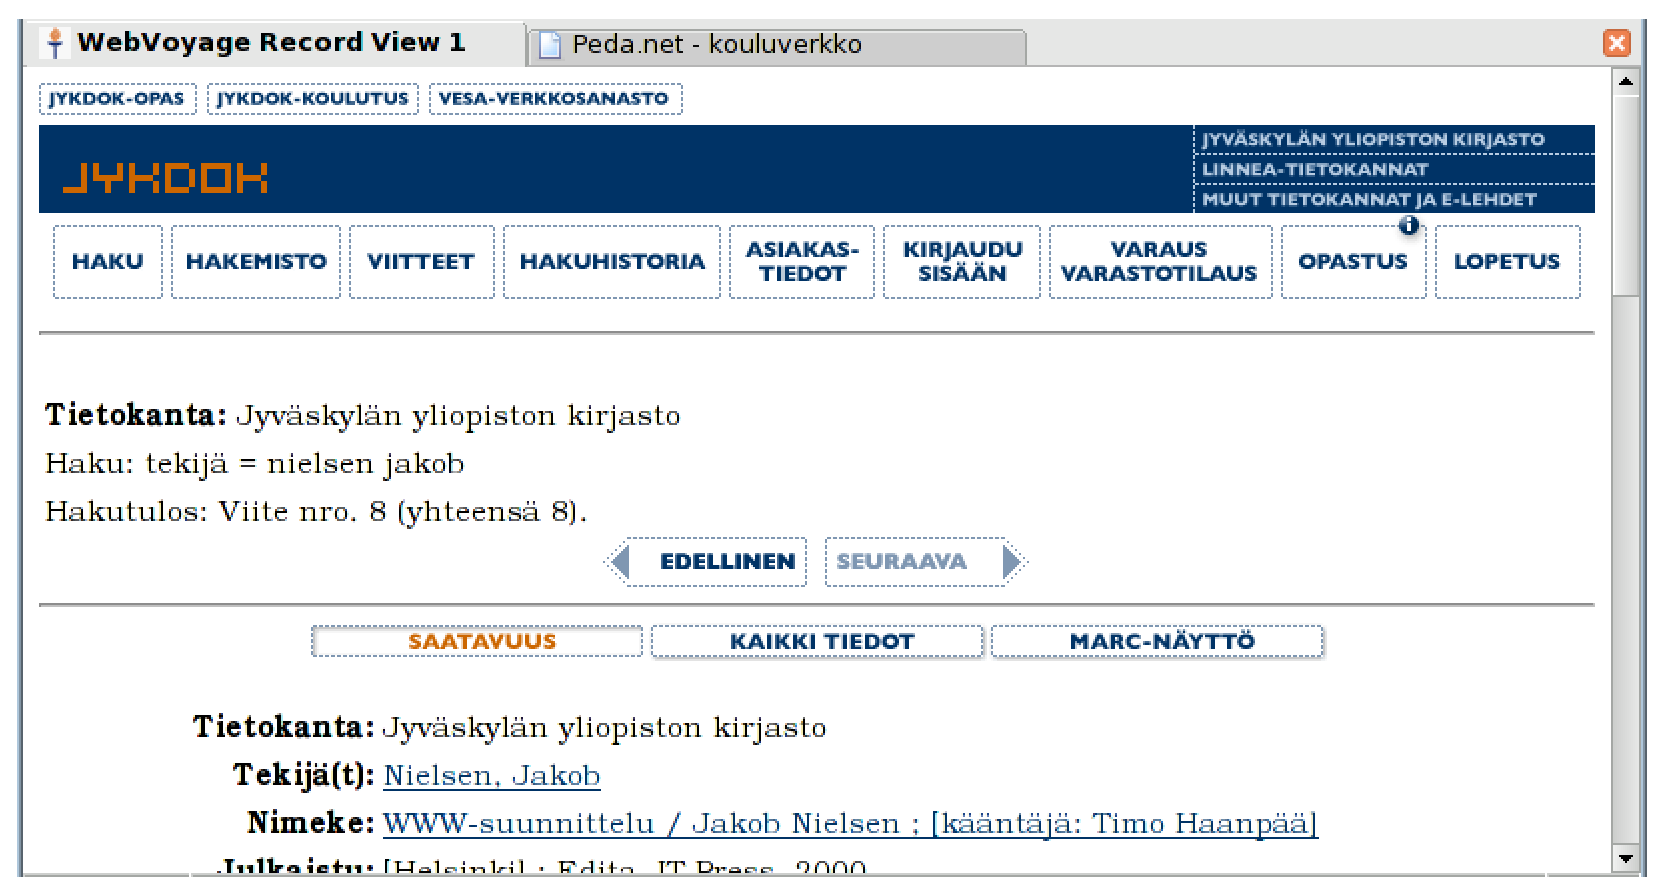
\includegraphics[width=14cm]{kuvat/kirjasto1}
\caption{Kirjaston hakupalvelun tulos}
\label{fig:kirjasto1}
\end{kuva}

Siirryn hetkeksi tarkistamaan toisessa selaimen ikkunassa, ett� t�m�
oli juuri se kirja, jota toisella sivustolla suositeltiin ja nostan
t�m�n ikkunan esiin muiden alta muutamaa minuuttia my�hemmin. Suureksi
h�mm�styksekseni juuri hakemani tiedot on hukattu, koska ``yhteytesi
tietokantaan on katkennut aikarajoituksen vuoksi'' (ks. kuva
\ref{fig:kirjasto2}). Ei minua k�ytt�j�n� kiinnosta mist� tiedot
haetaan ja erityisesti minua ei kiinnosta kuinka pitk�n yhteyden
tietokanta kerrallaan sallii. Palvelun tekij�ll� on selv�stikin ollut
ajatuksena valvoa n�in lyhyell� aikarajalla sit�, onko ikkuna viel�
aktiivisessa k�yt�ss�. Jostain syyst� on p��tetty, ett� jos k�ytt�j� ei
tee jotain muutaman minuutin sis�ll� niin silloin ``oikea'' toimenpide
on \emph{poistaa hakutulokset tai muu vastaava sis�lt�}. Sovellusta
tehdess� olisi ehk� kannattanut mietti�, olisiko sovellus mahdollista
toteuttaa siten, ett� tietokantapalvelimen aikarajan umpeutuessa
k�ytt�j�lle luovutettu sivu j�tet��n ennalleen ja huolehditaan
aikarajan umpeen menemisest� vasta, \emph{jos} k�ytt�j� viel� yritt��
tehd� jotain muuta.

\begin{kuva}
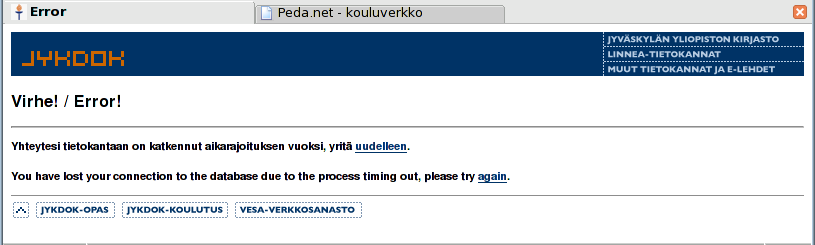
\includegraphics[width=14cm]{kuvat/kirjasto2}
\caption{Kirjaston hakupalvelun tulos kolme minuuttia haun j�lkeen}
\label{fig:kirjasto2}
\end{kuva}

\subsection{Selaink�ytt�iset ohjelmat tulee suunnitella toisin}

Tapahtumien avulla toimiva ohjelmalogiikka ei siis sin�ns� ole
syyllinen t�h�n ongelmaan, vaan se, ett� selaink�ytt�inen ohjelma ei
voi luottaa siihen, ett� kaikista asioista syntyisi tapahtuma. T�m�n
rajoituksen vuoksi sokeasti perinteisen mallin mukaisesti toteutettu
ohjelma toimii ep�vakaasti selaink�ytt�isen�.

\section{Perinteisten mallien sopimattomuus verkkoon}
\label{tiers}

Ohjelmistotuotannossa k�ytt�j�n kanssa vuorovaikutuksessa toimiva
ohjelmisto pyrit��n perinteisesti jakamaan kahteen tai kolmeen
kerrokseen. Kaksikerroksisessa mallissa (kuva \ref{fig:2tier}) ohjelman
logiikka erotetaan k�ytt�liittym�logiikasta ja kolmikerroksisessa
mallissa (kuva \ref{fig:3tier}) ohjelman logiikka jaetaan viel�
sovelluslogiikkaan ja tiedon k�sittelyn logiikkaan. Molemmissa
malleissa k�ytt�liittym� pidet��n omassa kerroksessaan erityisesti
siksi, ett� vaihtoehtoisen k�ytt�liittym�n rakentaminen olisi
mahdollisimman helppoa. K�yt�nn�ss� k�ytt�liittym�st� vastaava kerros
kutsuu melkein kaikkien toimintojen yhteydess� sovelluslogiikkaa ja
itse k�ytt�liittym�kerroksessa on kohtuullisen v�h�n ohjelmakoodia.
Voisi sanoa, ett� k�ytt�liittym�kerroksen teht�v� on tulkita
k�ytt�j�lle n�kyv�st� k�ytt�liittym�st� syntyneet tapahtumat eri
toiminnoiksi, jotka sitten edelleen ohjataan sovelluslogiikan
k�sitelt�v�ksi. T�m�n ansiosta ohjelma on yleens� helppo siirt��
esimerkiksi toimimaan jonkin toisen grafiikkakirjaston p��lle.
Kolmikerrosmallissa etuna on helppo siirrett�vyys my�s uudelle
tallennusmedialle.

\begin{kuva}
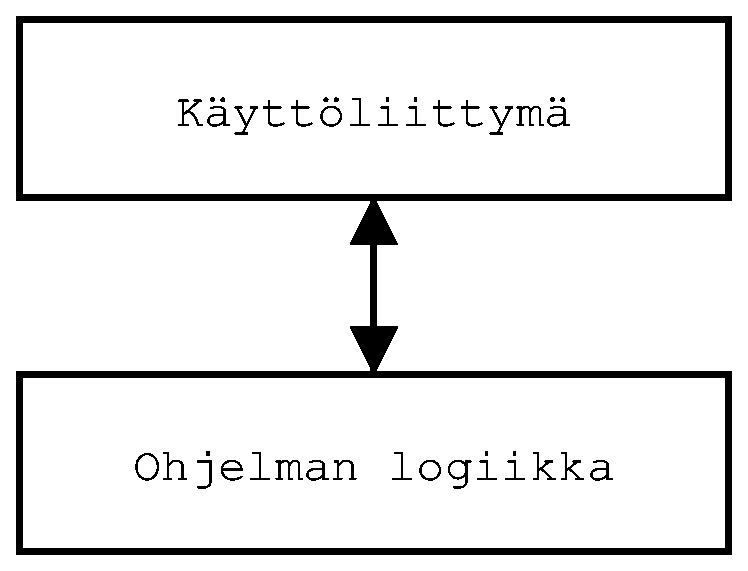
\includegraphics[width=5cm]{kuvat/fig2tier}
\caption{Kaavio kaksikerroksista ohjelma"-arkkitehtuurista}
\label{fig:2tier}
\end{kuva}

\begin{kuva}
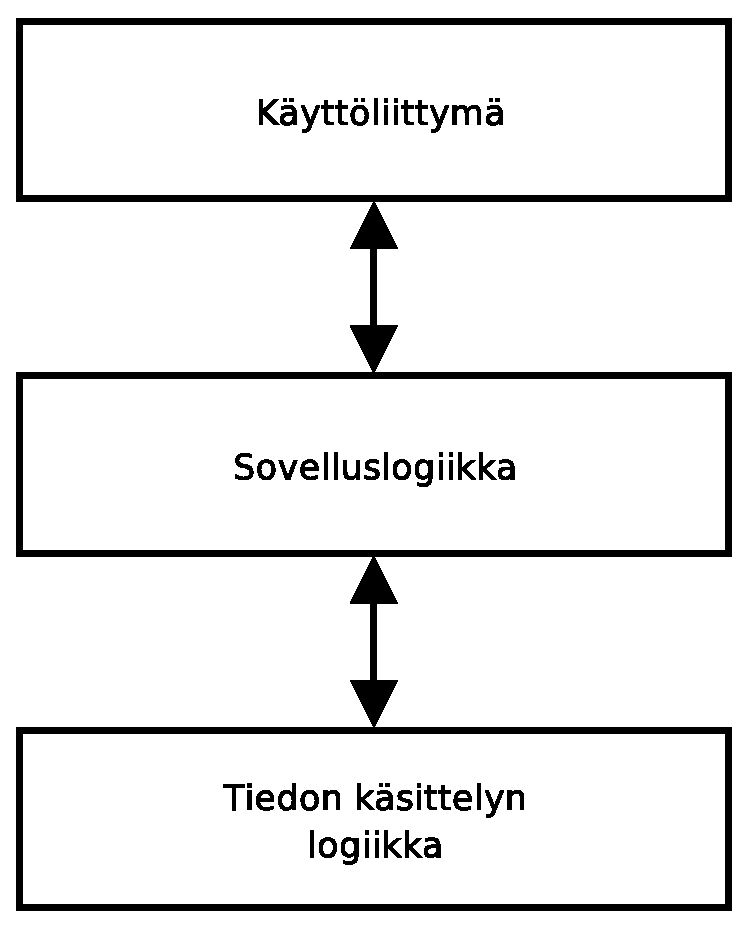
\includegraphics[width=5cm]{kuvat/fig3tier}
\caption{Kaavio kolmikerroksisesta ohjelma"-arkkitehtuurista}
\label{fig:3tier}
\end{kuva}

Verkossa toimivissa eli useinmiten selaink�ytt�isiss� ohjelmissa eteen
tulee perinteisess� mallissa kohtaamattomia ongelmia: k�ytt�liittym�n
toiminta on yhteydet�n, k�ytt�j� voi haarauttaa istunnon ja j�rjestelm�
ei voi erottaa verkon virheellist� toimintaa ja k�ytt�j�n hieman
tavallisesta poikkeavaa k�ytt�ytymist� toisistaan. Lis�ksi eri
selainohjelmien toteutuksissa on usein merkitt�vi� ohjelmavirheit�.
N�m� asiat kuuluvat k�ytt�liittym�kerrokseen, sill� ne eiv�t ole
ohjelman toimintalogiikan (eli sovelluslogiikan) kannalta olennaista
tietoa. Ongelmana vain on, ett� k�ytt�liittym�n toteutuksesta tulee
hyvin ty�l�s ja jos selaink�ytt�isi� ohjelmia tehd��n useita, joudutaan
k�ytt�liittym��n kuuluva kerros kirjoittamaan yh� uudelleen ja
uudelleen.

Teknisten ongelmien lis�ksi tulee ottaa huomioon my�s k�ytt�jien
tottumukset ja selainohjelmien p��asiallinen k�ytt�tarkoitus:
www"-sivujen selailu. Eri selainohjelmissa on erilaisia
erikoistoimintoja tavallisten sivujen selailun nopeuttamiseksi ja
tehostamiseksi. Jos selaink�ytt�ist� ohjelmaa ei voi k�ytt�� kuten
tavallisia www"-sivuja, joutuu k�ytt�j� opettelemaan j�lleen yhden
uuden ohjelman k�ytt�liittym�n ja h�n joutuu aina t�t� ohjelmaa
k�ytt�ess��n toimimaan eri tavalla kuin muilla www"-sivuilla. T�m�
lis�� k�ytt�j�n muistikuormaa ja heikent�� osaltaan sovelluksen
k�ytett�vyytt�.

\section{K�ytt�liittym�n esitt�minen verkon ehdoilla}

Verkossa toimivissa selainpohjaisissa k�ytt�liittymiss� perustavan
laatuinen ongelma on, ett� sivut tai k�ytt�liittym�n lomakkeet t�ytyy
esitt�� HTML"-kielen avulla. HTML on kuitenkin suunniteltu staattisten
dokumenttien esitt�miseen \cite{w3:html}. My�s
selaimet\footnote{HTML"-standardissa k�ytet��n sana ``selain'' sijasta
sanaa ``k�ytt�j�agentti'' korostamaan sit� seikkaa, ett� sivuja ei
v�ltt�m�tt� selailla, vaan tietokoneagentti -- ik��nkuin robotti -- k�y
k�ytt�j�n puolesta lukemassa sivuja ja tekee niist� vaikkapa
yhteenvetoja. Esimerkki usein k�ytetyst� agentista voisi olla Google.
My�s selain voisi hoitaa agentin teht�v�� ker��m�ll� sivustosta
esimerkiksi vain linkit normaalien sivujen n�ytt�misen sijasta.} on
suunniteltu p��asiassa staattisten sivukokonaisuuksien lukemiseen ja
sen vuoksi selaimissa onkin esimerkiksi \emph{takaisin}"-toiminto
(\alt{Back}). Lis�ksi selaimet k�ytt�v�t sivujen tiedonsiirrossa
HTTP"-protokollaa, jonka seurauksena k�ytt�liittym�t eiv�t ole koko
ajan yhteydess� palvelimen p��ss� toimivaan sovelluslogiikkaan.
Perinteiset k�ytt�liittymien suunnittelutavat ja toteutusmallit
soveltuvat huonosti selaink�ytt�isen k�ytt�liittym�n toteutukseen.
Esittelen seuraavassa muutamia suurimpia ongelmia, jotka syntyv�t
pohjalla olevista arkkitehtuurieroista. Tulee kuitenkin huomata, ett�
osa ongelmista syntyy siit�, ett� kokenut www"-selaimen k�ytt�j�
odottaa \emph{enemm�n vapauksia} ohjelman k�ytt�tavoissaan johtuen
siit�, ett� tavallisten www"-sivujen yhteydess� erilaisia k�ytt�tapoja
on useita. Hyv� selaink�ytt�inen ohjelma pystyykin vastaamaan n�ihin
odotuksiin.

\section{Yhteydet�n k�ytt�liittym�}

WWW"-selaimet k�ytt�v�t tiedon siirtoon HTTP"-yhteytt� tai SSL"-salattua
HTTP"-yhteytt� (t�st� k�ytet��n usein lyhennyst� \alt{HTTPS}). Molemmat
n�ist� yhteysmalleista ovat loogisesti yhteydett�mi�, vaikka
tehokkuuden vuoksi todelliset toteutukset pit�v�tkin yhteyden usein
auki eri dokumenttien noutamisen v�lill�. Selain voi milloin tahansa
katkaista entisen yhteyden ja luoda uuden, mutta t�m� ei saa vaikuttaa
ohjelman toimintaan.

Yhteydett�m�n toiminnan vuoksi k�ytt�liittym�n toiminnot t�ytyy
suunnitella siten, ett� yhdell� lomakkeella teht�v�t toiminnot eiv�t
vaadi ohjelman sis�lt��n puuttumista ennen seuraavalle lomakkeelle
siirtymist�. Ongelma voidaan osittain kiert�� k�ytt�m�ll�
JavaScript"-skriptikielt� asiakkaan selainohjelmassa, mutta koska
verkkoymp�rist�ss� asiakasohjelmaan ei voi luottaa, t�ytyy sama
sovelluslogiikka olla my�s palvelimen
p��ss�\footnote{JavaScript"-skriptikielell� voi esimerkiksi tarkistaa
onko sy�tekentt��n k�ytt�j�n kirjoittama tieto laskun viitenumero
laskemalla onko viitenumeron viimeinen tarkistusnumero oikein. Jos
tarkistusnumero ei toimi, n�ytet��n varoitusikkuna ja pyydet��n
k�ytt�j�� sy�tt�m��n tieto uudelleen. Kuitenkin, turvallisuussyist�
sama tarkistus t�ytyy tehd� my�s palvelimella (koska muuten
pahantahtoinen asiakas voisi muuttaa selaimessa toimivaa
JavaScript"-ohjelmaa ja l�hett�� virheellisen numeron j�rjestelm��n).}.
T�st� seuraa, ett� sama toiminnallisuus t�ytyy esitt�� kahdella eri
ohjelmointikielell� (JavaScript ja kieli, jolla palvelimen logiikka on
tehty). Seurauksena on koko j�rjestelm�n huomattavasti vaikeampi
yll�pito, koska eri kielill� tehtyjen toimintojen t�ytyy vastata
toisiaan. Vaihtoehtona on my�s toteuttaa kevyt tarkistus selaimen
p��ss�, jossa pyrit��n karsimaan suurimmat virheet pois, mutta sy�tetyn
tiedon oikeellisuus t�ytyy edelleen tarkistaa my�s palvelimen p��ss�.
Lis�ksi tulee huomata, ett� jos osa toiminnoista \emph{vaatii}
JavaScript"-kielen tukea, ei sovellus en�� toimi mill� tahansa
www"-selaimella.

\section{Ongelmallinen takaisin"-painike}

Kuten edell� mainitsin, selaimet on suunniteltu staattisten
dokumenttien k�ytt�miseen. Lis�ksi HTTP"-protokollan m��ritys erikseen
huomauttaa, ett� asiakasohjelman historiatietojen k�yt�n ei tarvitse
hakea tietoja palvelimelta \cite[kappale 13.13]{ietf:http}.
Esimerkkitapaus ongelmatilanteesta on esitetty kuvassa \ref{fig:fork}.
Esimerkiss� k�ytt�j� siirtyy ensin sovelluslogiikan luomalle sivulle
(lomakkeelle) $A$, valitsee toiminnon $a_1$ ja siirtyy sen seurauksena
sivulle $B$. T�m�n j�lkeen k�ytt�j� voi k�ytt�� selaimen
\emph{takaisin}"-toimintoa ja palata takaisin sivulle $A$. Koska t�m� on
siirtyminen selainohjelman historiatiedoissa, ei asiasta protokollan
mukaisesti tarvitse ilmoittaa palvelimelle, joten sovelluslogiikan
n�k�kulmasta asiakas on edelleen sivulla $B$. T�m�n j�lkeen asiakas
valitsee edellisest� poikkeavan toiminnon $a_2$. Palvelinohjelman tulee
t�ss� vaiheessa kyet� huomaamaan, ett� vaikka sen tarjoama lomake
olikin $B$, on k�ytt�j�n valitsema toiminto $a_2$ ja toimintoon
liittyv� tieto on per�isin lomakkeelta $A$, eik� lomakkeelta $B$.

Usein t�h�n ongelmaan k�ytetty ``ratkaisu'' on kertoa k�ytt�j�lle, ett�
sovelluksessa \emph{ei saa} k�ytt��
\emph{takaisin}"-toimintoa.\footnote{T�m� rajoitus seuraa yleens� siit�,
sovellus yritt�� pit�� istunnon tilaa yll�. Usein t�h�n k�ytet��n
keksej� (\alt{cookies}). N�iden suurin ongelma on, ett� niihink��n ei
voida helposti vaikuttaa historiatoimintojen yhteydess� ja lis�ksi ne
ovat globaaleja kaikkien selainohjelman ikkunoiden kesken. Jos istuntoa
kuvaavassa keksiss� s�ilytet��n my�s k�ytt�j�n tunnistetietoja ei
sovellukseen voi kirjautua monella eri k�ytt�j�tunnuksella
samanaikaisesti -- paitsi jos k�ytt�� eri selainohjelmaa jokaista
k�ytt�j�� kohden.} Olennaista on kuitenkin huomata, ett� k�ytt�j� teki
tietoisen p��t�ksen k�ytt�ess��n -- tai yritt�ess��n k�ytt�� --
kyseist� toimintoa ja varmastikin h�n olisi halunnut sen tekev�n jotain
muuta, kuin n�ytt�v�n virheilmoituksen.

%Ohjelma tulee siis tehd� sellaiseksi, ett� se pystyy vastaanottamaan ja k�sittelem��n \emph{mahdollisimman suuren} osan k�ytt�j�n l�hett�m�st� tiedosta, vaikka muuttuneen tilanteen vuoksi osa siit� ei olisikaan relevanttia.

\section{Istunnon haarautuminen}

Istunnon haarautuminen liittyy hyvin l�heisesti
\emph{takaisin}"-toimintoon. Siin� erona, k�ytt�j� kahdentaa aktiivisen
lomakkeen $A$ ja valitsee ensimm�isess� ikkunassa toiminnon $a_3$ ja
toisessa ikkunassa toiminnon $a_4$. J�rjestelm� palauttaa toiminnon
$a_3$ seurauksena sivun $C$ ja toiminnon $a_4$ seurauksena sivun $D$.
J�rjestelm�n kannalta t�m� tapahtuma n�ytt�� t�sm�lleen samalta kuin
\emph{takaisin}"-toiminnon k�ytt�kin, mutta merkitt�v� ero syntyy siit�,
ett� seuraavaksi k�ytt�j� voi tuottaa rinnakkaisia tapahtumia sek�
lomakkeelle $C$, ett� lomakkeelle $D$. Ei siis riit�, ett�
palvelinohjelma pit�� kirjaa k�ytt�j�n toimintahistoriasta ja osaa
peruuttaa l�hetettyjen kutsujen mukaan oikeaan tilanteeseen; lis�ksi
ohjelman pit�� kyet� haarauttamaan istuntoja ep�suorien tapahtumien
kautta. T�ysin oikean istuntoa kuvaavan tiedon yll�pit�minen
palvelimella onkin v�hint��nkin hyvin ty�l�st� ellei mahdotonta.
Istunnon tiedot t�ytyy siis jotenkin saada siirtym��n selainohjelmassa
ikkunakohtaisesti, jolloin ikkunan kahdentaminen kahdentaa my�s
istunnon.

\begin{figure}[htb]
\begin{center}
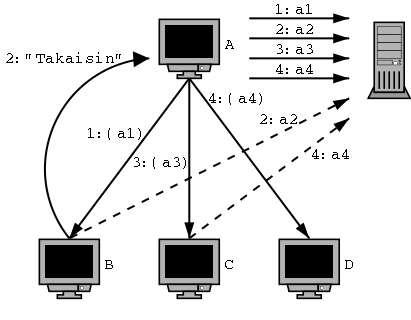
\includegraphics[width=10cm]{kuvat/fork}
\caption{Kaavio istunnon haarautumisesta}
\label{fig:fork}
\end{center}
\end{figure}

\section{Selaimen historia"-toiminnot}

Todellisuudessa takaisin"-painike ja uusien ikkunoiden avaaminen on vain
pieni osa itse varsinaista ongelmaa. Selaimet pit�v�t kirjaa kaikista
vierailluista sivuista ja koska selaink�ytt�isten sovellusten t�ytyy
esitt�� k�ytt�liittym�ns� HTML"-sivuina, kirjautuvat my�s t�llaisen
sovelluksen kaikki n�yt�t historia"-tietoihin. Sivuhistorian kautta
k�vij� voi palata \emph{suoraan mille tahansa sivulle} milloin tahansa.
Ei siis riit�, ett� varaudutaan siihen, ett� k�ytt�j� voi palata
edelliselle sivulle takaisin"-painikkeella, vaan kaikkien aikaisemmin
n�ytettyjen sivujen t�ytyy toimia.

Historiatoimintojen vuoksi ainoastaan takaisin"-painikkeen testaaminen
ei riit� testausvaiheessa. T�m�n seurauksena pelk�st��n takaisin- ja
eteenp�in "-painikkeiden testaaminen j�rjestelm�llisell� menetelm�ll�
\cite{lucca:web_application_testing} ei ole riitt�v�
testimenetelm� ohjelman oikean toiminnan varmistamiseksi.

K�yt�nn�ss� t�m� tarkoittaa sit�, ett� palvelimen p��ss� ei kannata
yritt�� pit�� kirjaa siit�, mik� n�kym� k�ytt�j�lle on annettu ja
erityisesti ei tule arvata, mik� n�kym� k�vij�n selaimessa on
aktiivinen.

\section{Verkon virheiden havaitseminen on mahdotonta}

Yhteydett�m�st� k�ytt�liittym�st� seuraa my�s, ett� palvelin ei voi
tunnistaa tietoverkon virheellist� toimintaa esimerkiksi asiakkaan
selaimen sulkemisesta tai asiakkaan tietokoneen jumiutumisesta.
Yll�mainitut ongelmatilanteet  n�kyv�t palveliohjelmalle t�ysin samalla
tavalla kuin, jos asiakas vain k�ytt�isi ep�tavallisen kauan aikaa
lomakkeen t�ytt�miseen. T�m�n vuoksi mik��n toiminto ei saisi lukittaa
resursseja siihen asti kunnes ``k�ytt�j�n istunto loppuu''. K�yt�nn�ss�
t�llaisia resurssien lukittamisia kuitenkin tarvitaan ja usein
ratkaisuna on k�ytt�� maksimiaikaa lukitukselle; kun k�ytt�j� valitsee
esimerkiksi uutisartikkelin muokattavaksi, merkit��n muokattava
artikkeli lukituksi, jolloin muut eiv�t voi sit� muokata. Lukitus
puretaan kun k�ytt�j� tallentaa muokatun artikkelin tai kun
ennaltam��r�tty maksimiaika lukitukselle on kulunut. T�ss�kin on
tietenkin ongelmana, ett� ongelmatilanteissa lukittu resurssi on
k�ytt�kelvoton valittuun aikarajaan asti. Parempi vaihtoehto olisikin
sallia rinnakkaisten muutosten tekeminen esimerkiksi versionhallinnan avustamana.

\section{Selainten virheelliset toteutukset}

Kun palvelimen ohjelmisto on saatu toimimaan ja kaikki edell�mainitut
ongelmat on otettu huomioon, havaitaan, ett� eri selainohjelmat eiv�t
toimi eri standardeissa m��r�tyll� tavalla. Useimmat vioista
vaikuttavat ainoastaan k�ytt�j�lle n�kyv�n lomakkeen ulkoasuun --
esimerkiksi joku teksti on suhteessa muuhun k�ytt�liittym��n
suuremmalla tekstill� kuin pit�isi. Kuitenkin osa vioista voi est��
tiettyjen toimintojen k�yt�n: esimerkiksi HTML"-m��rityksen mukaan
yhden \code{file}"-tyyppisen lomake"-elementin tulee tarjota
mahdollisuus usean tiedoston siirt�miseen yht� aikaa. Ainoa yleisesti
k�yt�ss� oleva selain, joka toimii t�ss� mieless� m��rityksen
mukaisesti, on Opera. T�m� n�kyy my�s yleisimmiss� palvelinp��n
toteutuksissa siten, ett� Operalla monta tiedostoa yht� aikaa
l�hetett�ess�, tapahtuu palvelinp��ss� yleens� virhe tiedostoja
vastaanotettaessa, koska palvelinohjelmiston kehitt�j� ei ole lukenut
m��rityst� vaan ainoastaan tarkkaillut kuinka yleisimm�t selaimet
toimivat. \cite{korpela:file_input}

Toinen yleinen virhe selainten toteutuksessa on tiedon l�hett�minen
UTF-8"-koodauksella ilman siit� ilmoittamista -- protokollan mukaan
oletuksena tulee t�ll�in k�ytt�� ISO-8859-1"-merkist��, jonka
seurauksena kaikki ASCII"-merkist�n ulkopuoliset merkit siirret��n
v��rin. T�ss� siis puutteellisen toiminnan lis�ksi tuhoutuu my�s
tietoa. T�m� ongelma voidaan kiert�� esimerkiksi l�hett�m�ll�
lomakkeella n�kym�t�n kentt�, jonka sis�lt� on tunnettu ja sis�lt��
ASCII"-merkist�n ulkopuolisia merkkej�, ja tarkastelemalla kuinka
selain koodaa t�m�n kent�n sis�ll�n.

\chapter{Ratkaisuja selaink�ytt�liittym�n toteutukseen}

\begin{chapterquote}{Keskustelu Matrix"-elokuvassa}
Neo: "You mean I can dodge bullets?"\\
Morpheus: "I mean when you are ready, you won't have to."
\end{chapterquote}

Kuten luvussa \ref{ongelmia} kuvasin, selaink�ytt�isten ohjelmien
k�ytt�liittymien toteuttamisessa on useita ongelmia. Kuvailen t�ss�
luvussa ratkaisuvaihtoehtoja tuossa luvussa kuvattujen ongelmien
ratkaisemiseksi. Osa suunnittelemistani ratkaisuvaihtoehdoista
osoittautui ep�k�yt�nn�llisiksi, mutta kuvailen ne siit� huolimatta
antamaan kuvaa ratkaisujen kehityskaaresta.

\section{K�ytt�liittym�kerroksen jakaminen osiin}

Ensimm�isen� ajatuksena oli jakaa luvussa \ref{tiers} kuvattu
kolmikerroksinen malli viel� kerran, p��tyen nelikerroksiseen
rakenteeseen. T�ss� mallissa k�ytt�liittym�kerros jaetaan
k�ytt�liittym�n toiminnallisuuden kuvaamiseen ja k�ytt�liittym�ajuriin
(kuva \ref{fig:4tier}).

\begin{figure}[htb]
\begin{center}
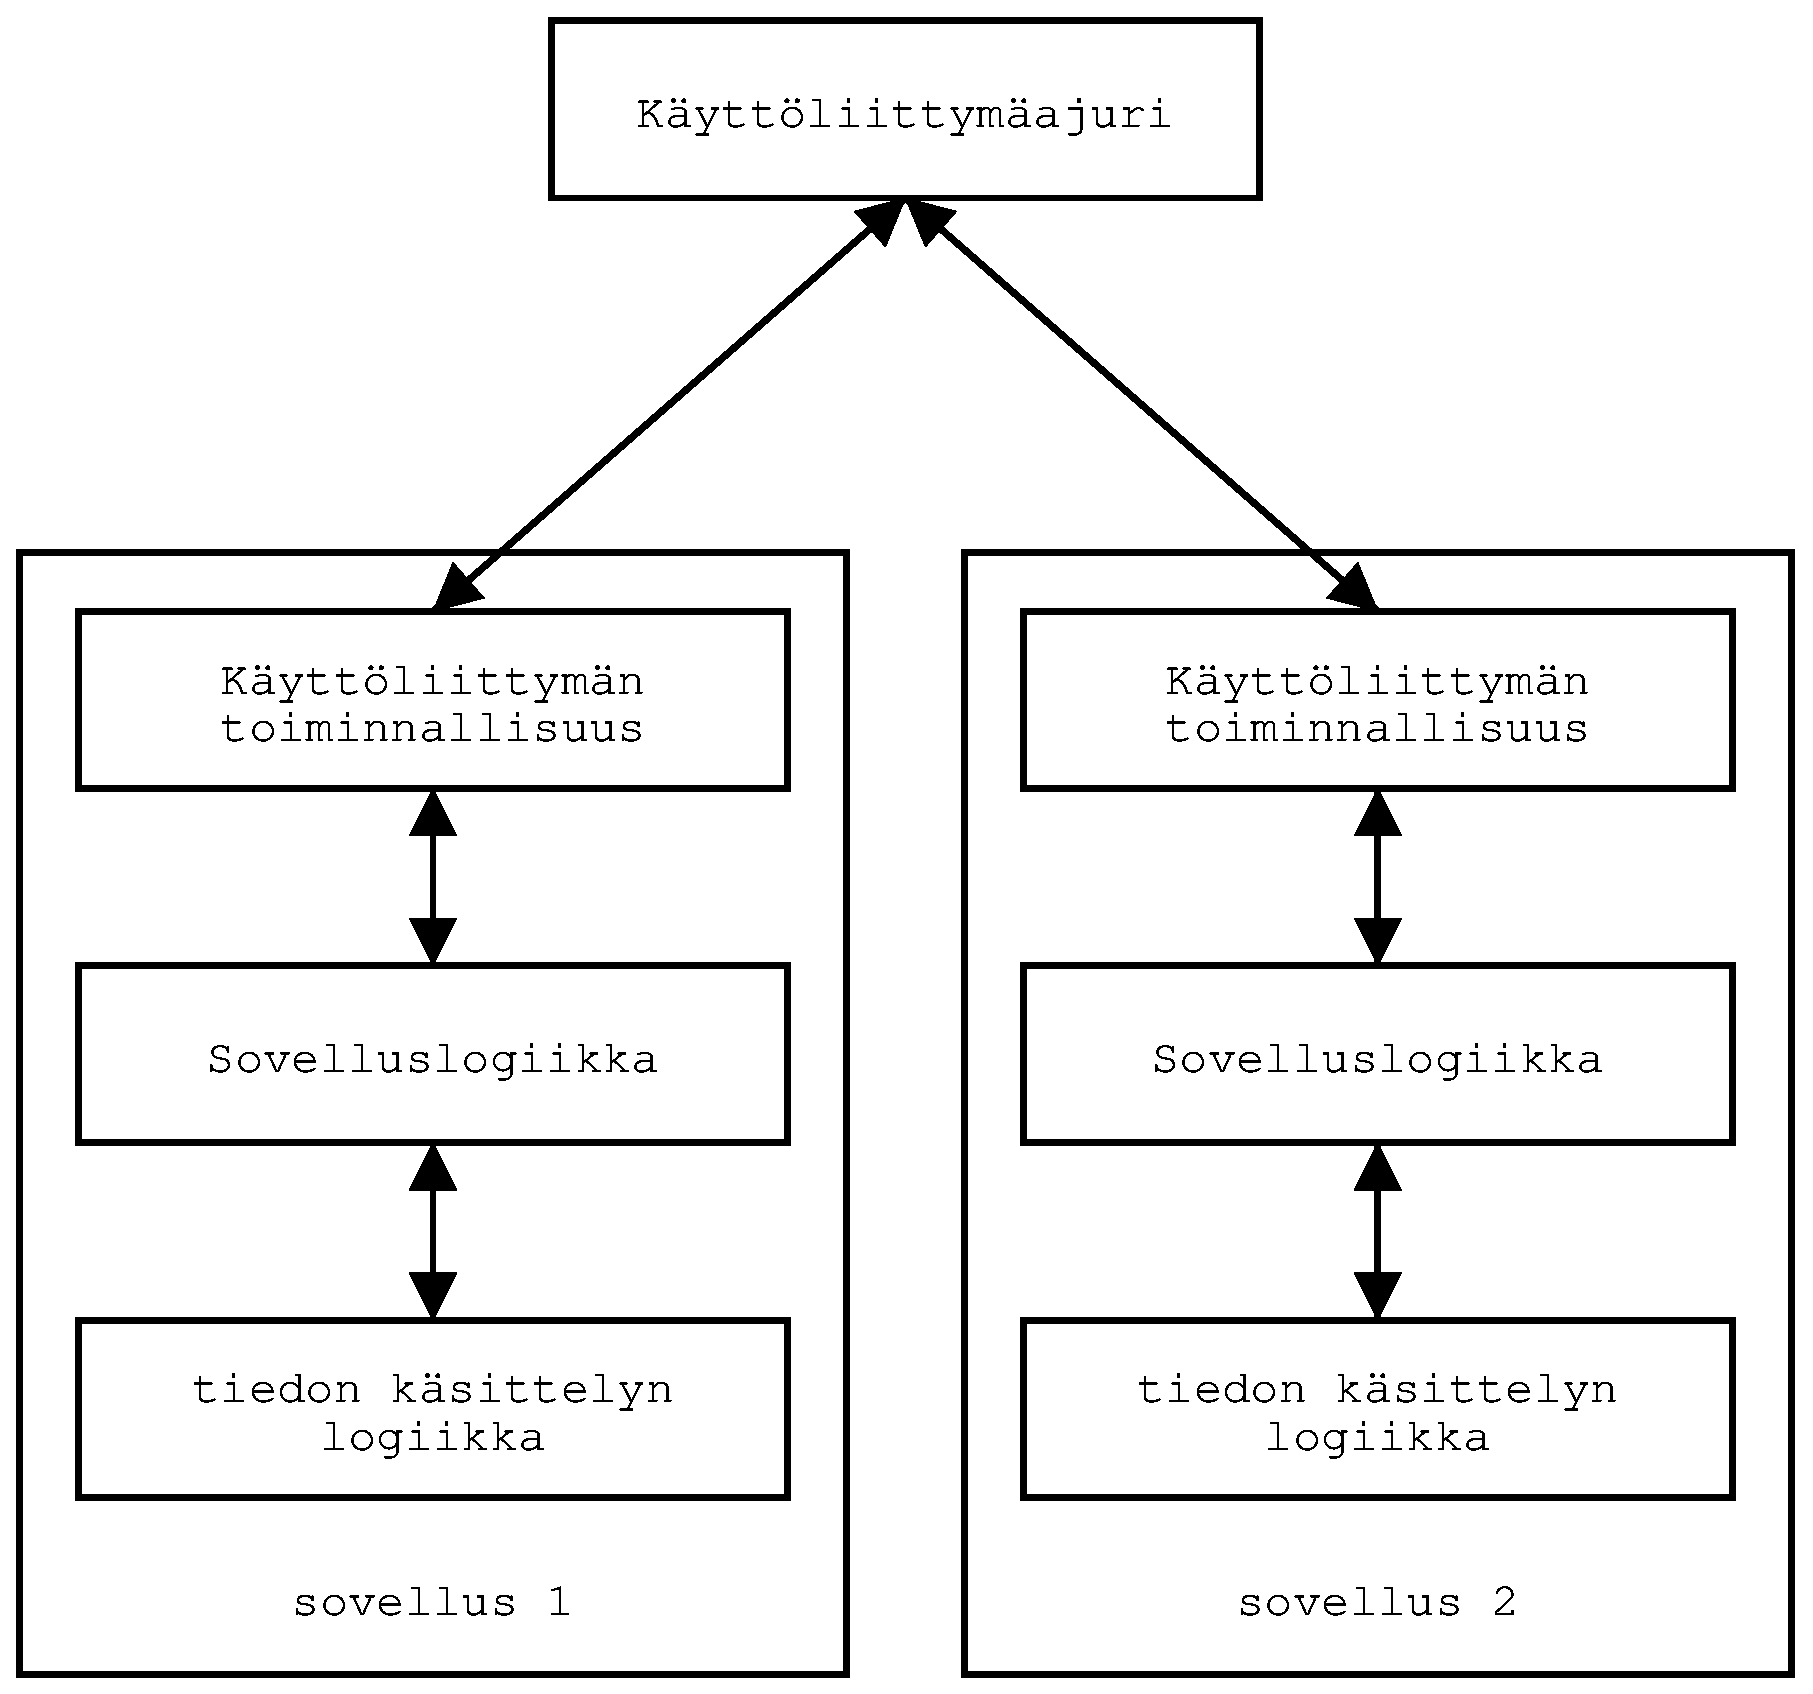
\includegraphics[width=10cm]{kuvat/fig4tier}
\caption{Kaavio nelikerroksista arkkitehtuurista usean sovelluksen
tapauksessa}
\label{fig:4tier}

\end{center}
\end{figure}

Jaon etuna eri sovellusten k�ytt�liittym�t saadaan toimimaan
vastaavalla ulkon��ll� ja mahdollisimman pitk�lti vastaavilla
toiminnoilla. T�m� onnistuu jakamalla k�ytt�liittym�ajuri eri
sovellusten kesken. Suunnittelemalla k�ytt�liittym�n toiminnallisuuden
ja k�ytt�liittym�ajurin rajapinta sopivasti, helpottuu k�ytt�liittym�n
kirjoittaminen verrattuna entiseen malliin, jossa k�ytt�liittym��
kirjoitettaessa jouduttiin kirjoittamaan koodi my�s k�ytt�liittym�n eri
osien, kuten erilaisten painikkeiden, hallintaan. Uudessa mallissa
k�ytt�liittym�n kuvauksessa vain ilmoitetaan, ett� k�ytt�j�n tulee
valita annetusta listasta kaksi tai kolme kohtaa. K�ytt�liittym�ajuri
voisi sitten toteuttaa tuon esityksen esimerkiksi ryhm�ll� \alt{radio
button} "=tyyppisi� grafiikkaelementtej� tai vaihtoehtoisesti
valintalaatikon (\alt{select box}) avulla. WWW"-k�yt�ss�
k�ytt�liittym�ajurin muodostamaa lopputulosta voitaisiin viel� hioa
kirjoittamalla lomakekohtaisia ulkon�k�asetuksia CSS"-kielell�
\cite{w3:css}.

K�ytt�liittym�ajuri keskustelee www"-selaimen kanssa, mutta
vaihtoehtoisesti sen voisi toteuttaa natiivilla sovelluksella. T�ll�in
edes ohjelman k�ytt�liittym�n kuvausta ei tarvitsisi muuttaa vaikka
k�ytt�ymp�rist� vaihtuisi selaink�ytt�isest� natiiviksi. Koska
toiminnallisuuden t�ytyy kuitenkin olla lomakepohjainen toimiakseen
\emph{hyvin} selaimen kautta, ei t�llainen natiivik�ytt�liittym� olisi
merkitt�v�sti parempi kuin selainpohjainen k�ytt�liittym�k��n.
V�it�nkin, ett� selaink�ytt�isten ohjelmien k�ytt�liittymien logiikka
ja dialogien rakenne pit��kin suunnitella eri tavalla kuin
perinteisten, k�ytt�j�rjestelm�n omien s��nt�jen mukaan toimivien
sovellusten.

\subsection{Tiedon k�sittelyn logiikka}

T�m� kerros toteutetaan k�ytt�m�ll� jotain olemassaolevaa tietokantaa,
esimerkiksi MySQL tai PostgreSQL. Teoriassa tietokannan pit�isi
ymm�rt�� ja valvoa kaikki tiedon esitysmalliin liittyv�t rajoitukset.
K�yt�nn�ss� t�h�n ei p��st�, koska rajanpinta tiedon k�sittelyn
logiikan ja sovelluslogiikan v�lill� on toteutettu SQL"-kielell�. Monien
tietokantojen tuki SQL"-kielelle on varsin kehittym�t�n erityisesti
tietorakenteen rajoitusten suhteen. T�m�n seurauksena merkitt�v� osa
tiedon esitysmallin rajoituksista joudutaan sijoittamaan
sovelluslogiikkaan. Muuten sovellusta ei voida tulevaisuudessa siirt��
toimimaan toisen tietokannan p��ll�. Jos siirrett�vyys ei ole
tavoitteena, tietokannan tehokkuus voidaan maksimoida ohjelmoimalla
tarkistukset ja rajoitukset tietokannan omilla ty�kaluilla. Pyrin itse
pit�m��n selaink�ytt�iset sovellukset tietokantariippumattomina -- eli
sijoitan rajoitukset sovelluslogiikkaan -- koska olen kokenut, ett�
k�yt�nn�ss� eri tietokannan k�ytt�misest� saatava nopeusero on suurempi
kuin yksitt�isen tietokannan hienos��t�misest� saatava nopeusero.
Toisin sanoen, suurin nopeuden kasvattaminen saataisiin aikaiseksi
vaihtamalla tietokantaa aina sen hetkisen sis�ll�n ja k�ytt�profiilin
mukaisesti nopeiten toimivaan. T�m�n tutkielman kannalta tarkka jako
tiedon k�sittelyn logiikan ja sovelluslogiikan v�lill� ei ole
kuitenkaan olennaista.

\subsection{Sovelluslogiikka}

Sovelluslogiikka vastaa sovelluksen ``�lyst�''. Teoriassa t�ss�
kerroksessa ei oteta mit��n kantaa sovelluksen k�ytt�liittym��n.
K�yt�nn�ss� t�m� kerros on todenn�k�isesti tehokkainta sulauttaa
osittain k�ytt�liittym�n toiminnallisuuden kanssa. N�in sen vuoksi,
ett� sovelluslogiikkaan ei yleens� ohjelmoida ominaisuuksia, joita
k�ytt�liittym�n toiminnallisuus ei tarvitse. Toisaalta k�ytt�liittym��n
ei voida lis�t� ominaisuuksia, joita sovelluslogiikka ei tue. Eli
kaikki muutokset t�ytyy kuitenkin tehd� molempiin osiin, jonka vuoksi
jaosta ei saada kovin paljon etua. Lis�ksi sulauttamisen haittojen voi
nelj�n kerroksen mallissa olettaa olevan kohtuullisen pieni�, koska
k�ytt�liittym�n toiminnallisuus ei ole en�� tiukasti sidottu itse
k�ytt�liittym�n ulkon�k��n.

\subsection{K�ytt�liittym�n toiminnallisuus}

K�ytt�liittym�n toiminnallisuudesta vastaava kerros kuvaa
k�ytt�liittym�n toiminnan abstraktilla tavalla: ``t�st� taulukosta
t�ytyy valita 2--5 rivi�'' tai ``k�ytt�j�n tulee sy�tt�� lomakkeelle
kaksi merkkijonoa. N�iden merkkijonojen nimet ja tyypit ovat
`k�ytt�j�tunnus':merkkijono ja `salasana':salattu merkkijono.'' T�m�
kerros ei ota kantaa siihen miss� j�rjestyksess� taulukon sarakkeet ja
rivit n�ytet��n tai siihen, sy�tet��nk� k�ytt�j�tunnus tekstikentt��n
vai vaikkapa napauttelemalla hiirell� jonkin kuvan eri kohtia.

Teoriassa t�m� kerros voisi generoida yksinkertaisen XML"-sivun, joka
muutettaisiin XHTML tai HTML "=sivuksi selaimen toimintoja varten.
T�ll�in k�ytt�liittym�ajurin voisi kirjoittaa esimerkiksi
XSLT"-kielell�. K�yt�nn�ss� t�llaisen ajurin kirjoittaminen muodostuu
oletettavasti niin hankalaksi, ett� paremmalta vaihtoehdolta tuntuu
kirjoittaa k�ytt�liittym�ajuri kirjastoksi, joka
linkitet��n\footnote{Joissakin ohjelmointiymp�rist�iss� ohjelmakoodi
k��nnet��n objektitiedostoiksi, jotka yhdistet��n \emph{linkitt�m�ll�}
valmiin ohjelman tuottamiseksi. Vasta n�in tuotettu valmis ohjelma
voidaan suorittaa. Toisaalta, esimerkiksi PHP"-kielisiss� ohjelmissa
manuaalinen linkitys ei ole tarpeen, sill� se suoritetaan
automaattisesti ohjelman k�ynnistyess� kun kirjastoa on muutettu.}
ohjelmaan sit� teht�ess�. Linkitys pit�� tehd� uudelleen kirjaston
p�ivityksen yhteydess�, mutta itse k�ytt�liittym�n toiminnallisuuteen
ei tarvitse puuttua. T�ss�kin mallissa eri sovellusten k�ytt�liittym�t
saadaan s�ilym��n yhdenmukaisina pelk�st��n linkitt�m�ll� kaikki
sovellukset uudelleen aina k�ytt�liittym�ajurin p�ivityksen j�lkeen.
\cite{w3:xml_v1_0,w3:xhtml,w3:xslt}

\subsection{K�ytt�liittym�ajuri}

T�m� kerros vastaa siit� kuinka k�ytt�j� pystyy tekem��n eri valinnat
ja toiminnot. Jos, k�ytt�liittym�ss� on kuvattu, ett� lomakkeella on 10
vaihtoehtoa, joista pit�� valita t�sm�lleen yksi, niin t�ll�in
selaink�ytt�isen sovelluksen k�ytt�liittym�ajuri voi n�ytt�� sivulla 10
linkki�, joista k�ytt�j� painaa yht�. \emph{Vaihtoehtoisesti} ajuri
voisi n�ytt�� lomakkeen jossa on 10 \alt{radio button} "=tyyppist�
elementti� ja OK"-painike. Kolmas vaihtoehto olisi n�ytt��
\alt{combobox}"-alasvetovalikko yhdistettyn� JavaScript"-k�sittelij��n,
joka l�hett�isi lomakkeen v�litt�m�sti k�ytt�j�n n�p�ytetty� jotain
kohtaa. Optimaalisessa tapauksessa k�ytt�liittym�ajuri osaisi k�ytt��
kaikkia n�it� vaihtoehtoja ja k�ytt�j� voisi omissa asetuksissaan
valita mill� tyylill� h�n haluaa k�ytt�� erityyppisi� lomakkeita.

\subsection{K�ytt�liittym�ajurille j�� paljon vastuuta}
\label{kaikki-data-sivulla}

Koska selaink�ytt�isen sovelluksen k�ytt�j� voi esimerkiksi haarauttaa
istunnon ja t�st� toiminnosta ei synny tapahtumaa palvelimelle, t�ytyy
kaikki tieto kuljettaa lomakkeen muun tiedon yhteydess� sivuun
upotettuna. T�ll�in tieto kahdentuu automaattisesti, kun k�ytt�j�
kahdentaa istunnon eli k�yt�nn�ss� avaa uuden ikkunan, jossa on sama
sovellus toiminnassa. Samoin historiatoimintojen yhteydess� selain
k�ytt�� automaattisesti entisen lomakkeen tietoja, sill� nuo tiedot
sis�ltyv�t siihen sivuun, jota selain k�ytt�� sivun n�ytt�miseenkin.
K�ytt�liittym�ajuri ei voi est�� vanhentuneen tiedon saapumista, joten
k�ytt�liittym�n toiminnallisuuden tai sovelluslogiikan t�ytyy ottaa
siihen kantaa.\footnote{K�ytt�j� voisi esimerkiksi muokata
selaink�ytt�liittym�ll� uutisartikkelia, poistaa artikkelin ja k�ytt��
\emph{takaisin} toimintoa palatakseen takaisin muokkaus-toimintoon. Kun
k�ytt�j� nyt tallentaa tehdyt muokkaukset t�ytyy sovelluksen joko
palauttaa poistettu artikkeli tai luoda l�hetettyjen tietojen
perusteella uusi tai k�ytt�j�n l�hett�m�� tieto hukkuu.}

Istunnon yll�pitoon tarvittavan tiedon m��r�n t�ytyy olla pieni, koska
kaikkien sovelluksen generoimien sivujen sis�lt�mien linkkien t�ytyy
sis�lt�� my�s istunnon tiedot.\footnote{WWW"-sivulla olevat linkit
k�ytt�v�t aina GET"-metodia HTTP"-yhteyksi� k�ytett�ess�, jossa kaikki
linkin parametrit pit�� siirt�� tekstin� osoitteen lopussa. Istuntoon
liittyv�t tiedot t�ytyy siis toistaa sivun \emph{jokaisen} linkin
lopussa ja sivu kasvaa huomattavan nopeasti linkkien lukum��r�n mukaan
jos istunto"-tietoa on paljon.} HTTP"-protokolla m��rittelee
tavallisten linkkien k�ytt�m�n GET"-toiminnon maksimidatam��r�ksi nelj�
kilotavua, joka asettaa yl�rajan istunnon koolle.
\cite{ietf:http}

Koska \emph{kaikkien} sovellusten tietojen l�hett�minen jokaisen
lomakkeen yhteydess� vaatisi huomattavan lis�n tarvittavaan
tiedonsiirtokaistaan, tulee ohjelman toteutuksessa erikseen jakaa
istunto"-tiedot kahteen osaan: lomakkeiden kautta siirtyv� tieto, ja
tieto, joka voidaan jakaa my�s haarautettujen tai vanhentuneiden
tapahtumien kanssa. T�ll�in jaettu tieto voidaan s�ilytt��
palvelimella. T�llaista jaettua tietoa olisivat esimerkiksi k�ytt�j�n
henkil�kohtaiset asetukset, jotka voidaan jakaa eri ikkunoiden kesken.
Esimerkiksi valittu koko sivuston tyyli tai p�iv�m��rien esitysmuoto
olisi t�llaista tietoa. Jakamatonta istuntotietoa olisi taas
esimerkiksi tieto siit�, mit� toimintoja k�ytt�j� k�ytti saapuessaan
nykyiseen n�kym��n, jos t�t� tietoa tarvitaan tulevaisuudessa.

Tulevaisuudessa selaink�ytt�isen sovelluksen k�ytt�liittym�ajuri voisi
esitt�� k�ytt�liittym�n XForms"-m��rityksen mukaisilla lomakkeilla,
jolloin k�ytt�liittym�n toiminnallisuus ja ulkon�k� voidaan pit��
erill��n www"-selaimeen asti. Ik�v� kyll� XForms on hyvin heikosti
tuettu uusimmissakin selaimissa ja mik��n ei viittaa siihen, ett�
tilanteeseen olisi tulossa nopeasti muutosta.
\cite{korpela:html_forms,w3:xforms}

\subsection{Huomioita k�ytt�liittym�ajurin toteuttamiseen liittyen}

Koska eri selaimissa on erilaisia vikoja, ei k�ytt�liittym�ajuri voi
ainoastaan tuottaa standardinmukaisia lomakkeita, vaan sen t�ytyy
yritt�� tunnistaa asiakasohjelma (selaintyyppi ja versio) ja kiert��
jollakin tavalla siin� tunnetut ongelmat. Viallisten selainten tukeen
kuluva ty�aika on helpompi perustella, koska ajuri on yhteinen monelle
eri sovellukselle, joten kustannukset ohjelmaa kohden ovat pienempi�
kuin perinteisell� mallilla. Er�iss�, erityisesti ulkon�k��n liittyviss�
yksityiskohdissa, samaan lopputulokseen on mahdollista pyrki� usealla
eri tavalla standardin puitteissa ja n�ist� t�ytyy kokeilemalla etsi�
se malli, joka toimii eri selaimissa. T�ll�in eri selaimia varten ei
tarvitse kirjoittaa selainkohtaisia ominaisuuksia.

Koska k�ytt�liittym�ajurin t�ytyy huolehtia kaikista selaimen k�yt�st�
johtuvista ongelmista, on sen toteuttaminen vaikeaa. HTML"-kielt�
tukevan ajurin ei kuitenkaan tarvitse ottaa kantaa k�ytt�liittym�n
yksityiskohtiin, ainoastaan eri komponenttien j�rjestykseen, sill�
ulkon��lliset yksityiskohdat, kuten v�rit ja elementtien asemoinnit
voidaan k�sitell� vasta selaimessa k�ytt�j�n tietokoneella CSS"-kielen
avulla \cite{w3:css}. Sovellukselle voidaan helposti tuottaa erilaisia
ulkoasuja (\alt{skins}) pelk�st��n luomalla erilaisia CSS"-tiedostoja.
Lis�ksi standardi mahdollistaa eri CSS"-tiedostojen kirjoittamisen
esimerkiksi normaalille selaimelle, dataprojektorille ja
k�mmentietokoneille; k�ytt�liittym�n ulkoasu on siis mahdollista hioa
tarvittaessa laitekohtaisesti.

\section{Nelikerroksisen mallin k�yt�nn�n ongelmia}

Aloin toteuttamaan k�ytt�liittym�ajuriajatusta Peda.net"-hankkeessa
teht�v�n Oppimappi"-nimisen ty�kalun
valmistuksessa\footnote{Oppimappi"-ty�kalusta kerrotaan tarkemmin
luvussa \ref{pedanet-oppimappi}}. Peda.net"-hankkeessa on p��tetty
yhdenmukaistaa sovellusten toimintaymp�rist�ksi Apache"-www"-palvelimen
p��ll� toimiva PHP"-ohjelmointiymp�rist� sek� MySQL"-tietokanta, joten
t�m� asetti k�yt�nn�n rajoituksia ohjelman loogiseen rakenteeseen;
nykyisin k�yt�ss� oleva PHP"-kielen versio 4 ei tue moniperint�� eik�
rajapintaluokkia, joten luokkahierarkian toteuttaminen vaati osin
teoriittisesta mallista poikkeamista.

% Oppimappia voi k�ytt�� sek� MySQL
% ett� PostgreSQL "=tietokantojen p��ll�. Nykyisell� palvelimella MySQL
% toimii nopeammin.

Kuvassa \ref{fig:oppimappi-schema-orig} on esitetty osa alkuper�isest�
luokkahierarkiasta.

%Kuvassa \ref{fig:oppimappi-big-picture} on puolestaan
%mallinnettu ymp�rist�� isommassa mittakaavassa. K�yt�nn�ss�
%MySQL"-tietokanta ja Oppimappi PHP"-sovellus toimivat
%Peda.net"-hankkeen yll�pit�m�ll� palvelimella ja ohjelman
%k�ytt�liittym� esitet��n HTML ja CSS "=kielien avulla sovelluksen
%k�ytt�j�n koneessa toimivassa www"-selaimessa.

\begin{kuva}
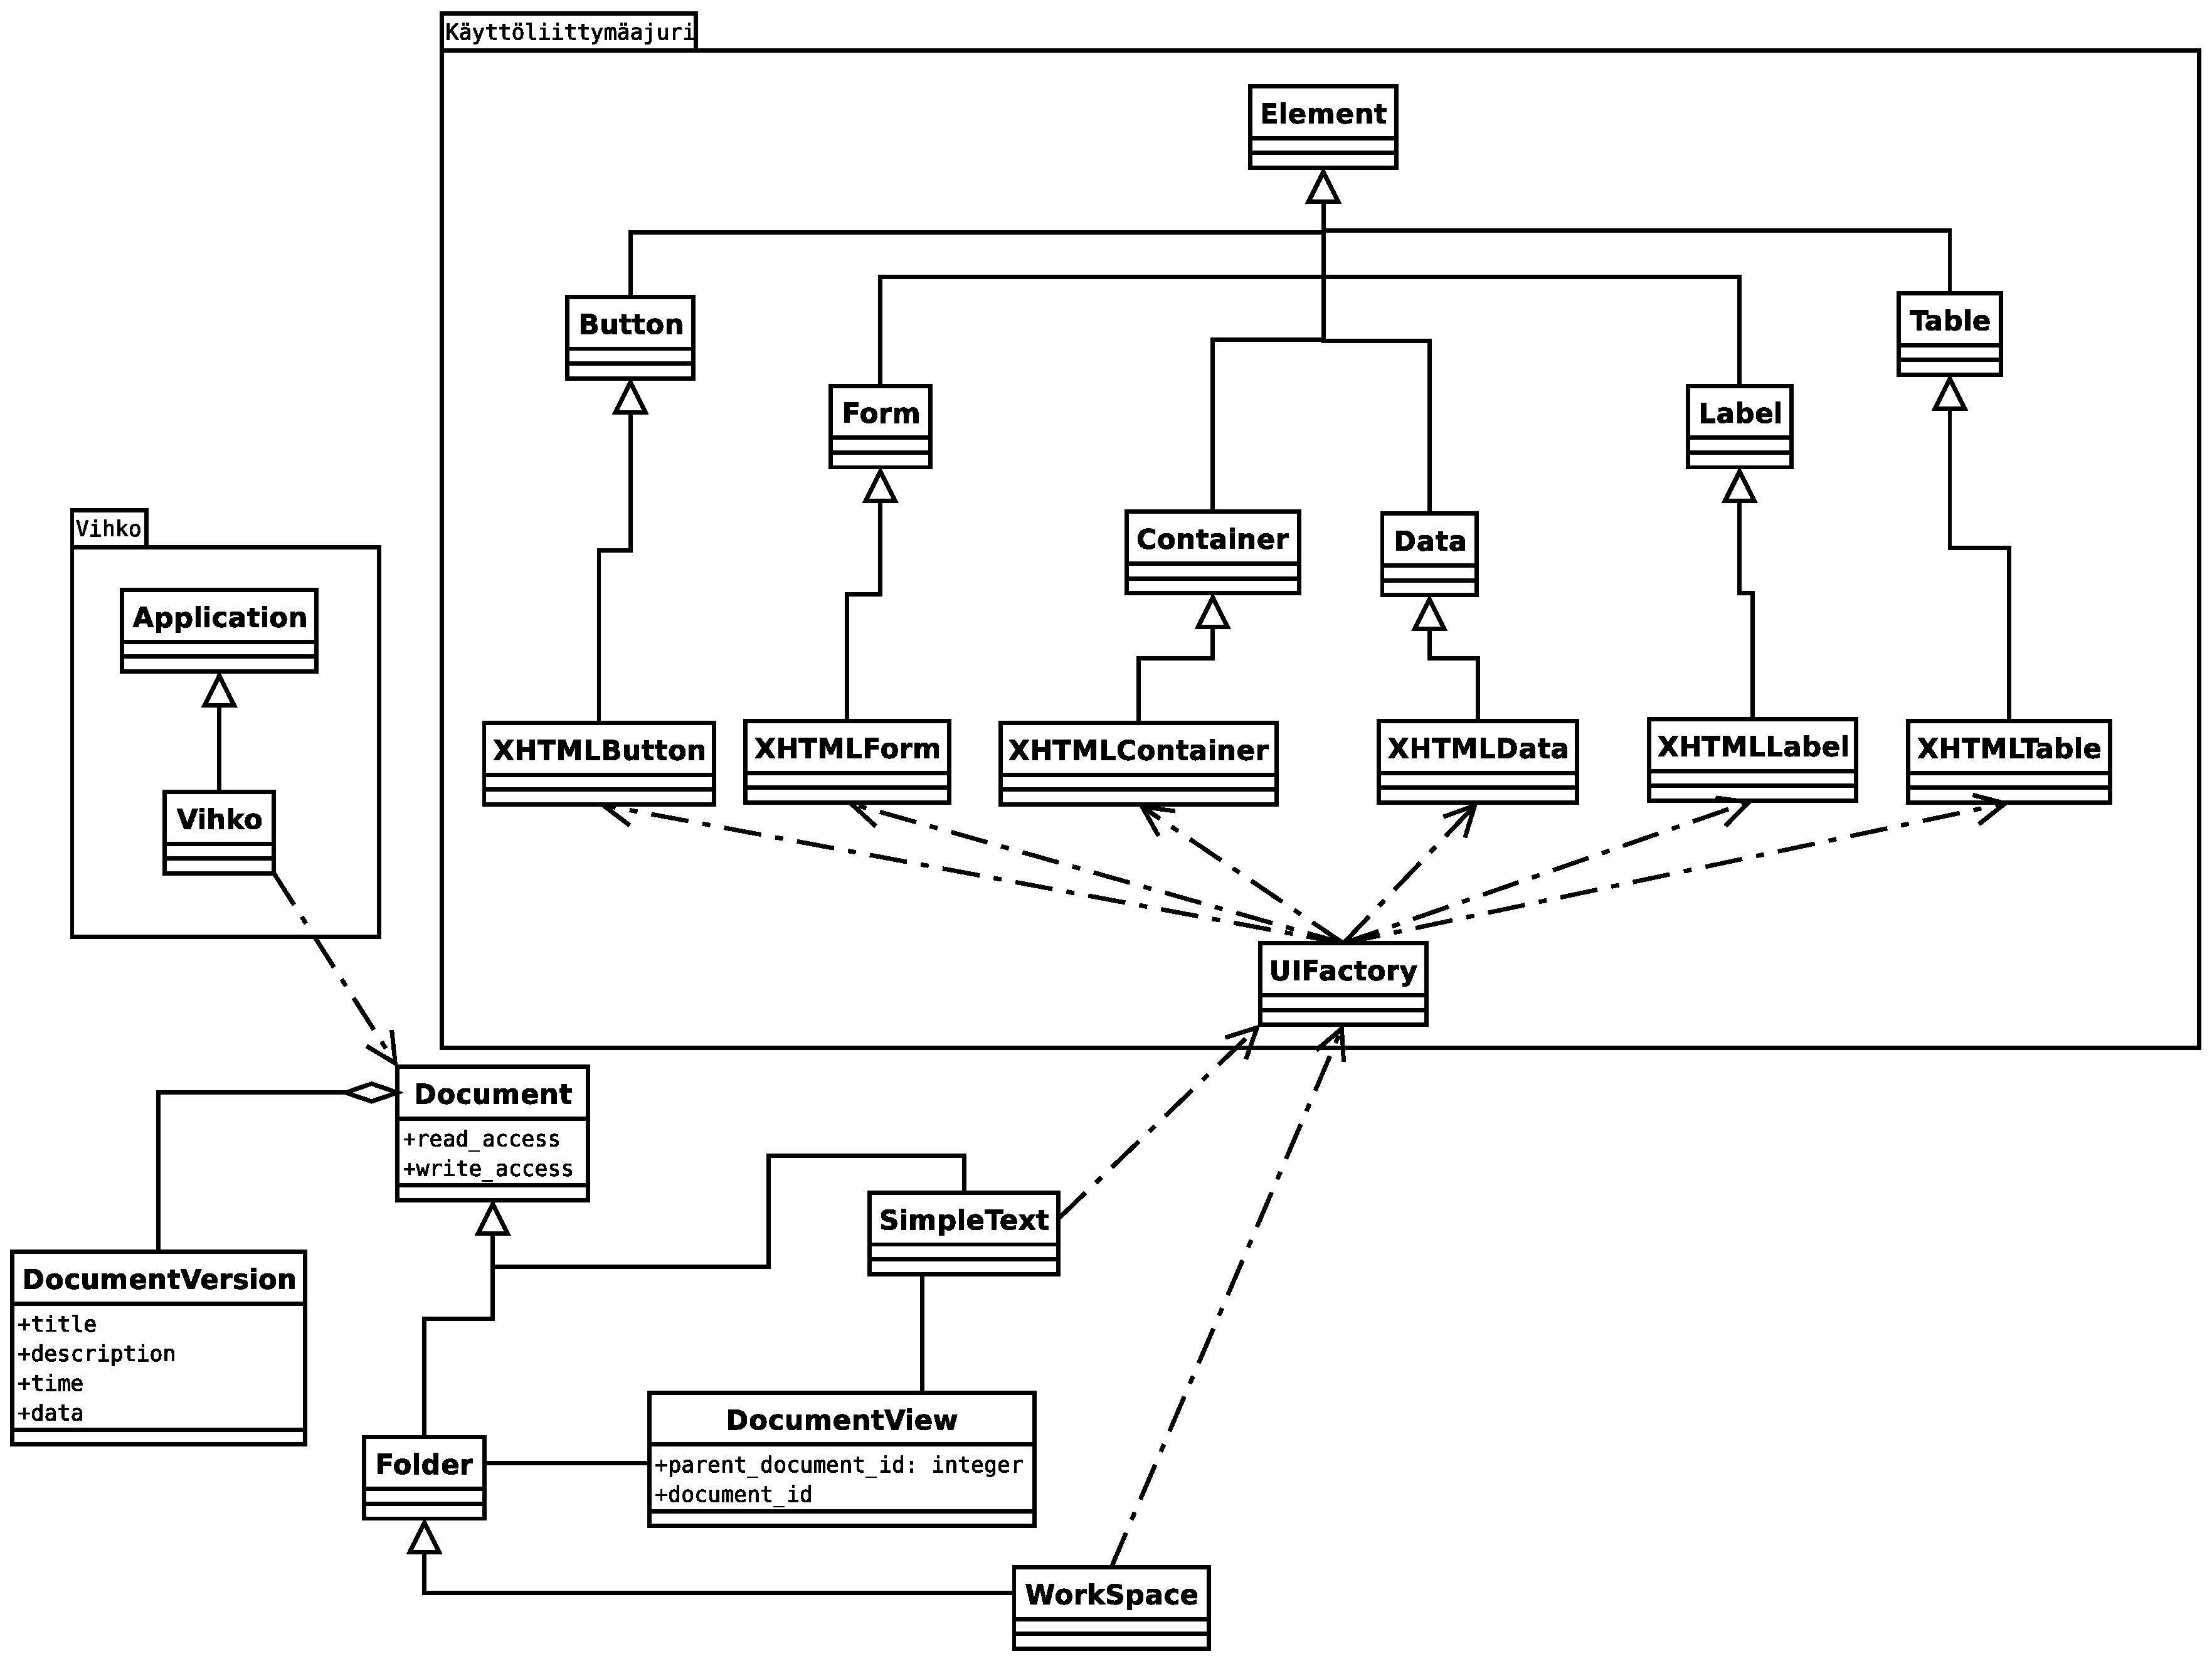
\includegraphics[width=\linewidth]{kuvat/oppimappi-schema-orig}
\caption{Alkuper�ist� suunnitelmaa Oppimapin toteuttamiseksi}
\label{fig:oppimappi-schema-orig}
\end{kuva}

Noin kuukauden kehitysty�n j�lkeen k�vi kuitenkin selv�ksi, ett�
PHP"-ymp�rist�n suorituskyky olioiden luomisessa ja tuhoamisessa oli
aika heikko. Lis�ksi t�ydellisen k�ytt�liittym�ajurin tekeminen alkoi
varmistumaan liian ty�l��ksi siit� saataviin etuihin verrattuna.

\section{K�ytt�liittym�ajurin yksinkertaistaminen}

P��dyin siihen johtop��t�kseen, ettei t�ydellist� k�ytt�liittym�ajuria
kannata tehd�, koska varsinaisen sovelluslogiikan ja k�ytt�j�n
v�liss� on niin useita tasoja. Jakamalla k�ytt�liittym� sopivasti HTML
ja CSS -kielien vastuulle, k�ytt�liittym�ajuri voidaan pit�� hyvin
yksinkertaisena. T�t� on havainnollistettu kuvassa
\ref{fig:oppimappi-big-picture}. Lis�ksi, koska PHP rajaa ainakin
toistaiseksi natiivin k�ytt�liittym�n kehitt�misen mahdollisuuksia
suoritusymp�rist�ns� vuoksi, ei natiivisovelluksen kehitt�misen
helpottamiseksi kannattanut t�ss� vaiheessa uhrata aikaa.

\begin{kuva}
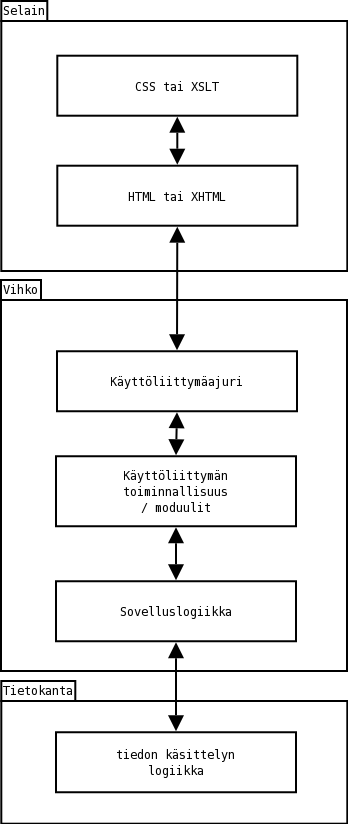
\includegraphics[width=4.2cm]{kuvat/oppimappi-big-picture}
\caption{Oppimapin rakenne kerroksina}
\label{fig:oppimappi-big-picture}
\end{kuva}


Kuvassa \ref{fig:oppimappi-schema-current} on  esitetty Oppimapissa
loppujen lopuksi k�ytetty ratkaisumalli. T�ss�kin luokkahierarkia on
hieman erikoinen, mutta ratkaisun taustalla kummittelee vaillinainen
oliotuki PHP-kieless�. T�t� kirjoittaessa PHP"-kielen versio 5 on jo
ilmestynyt ja siin� osa puutteista onkin korjattu, mutta sen
tuotantok�ytt�� kannattanee harkita aikaisintaan ensi vuonna.

\begin{kuva}
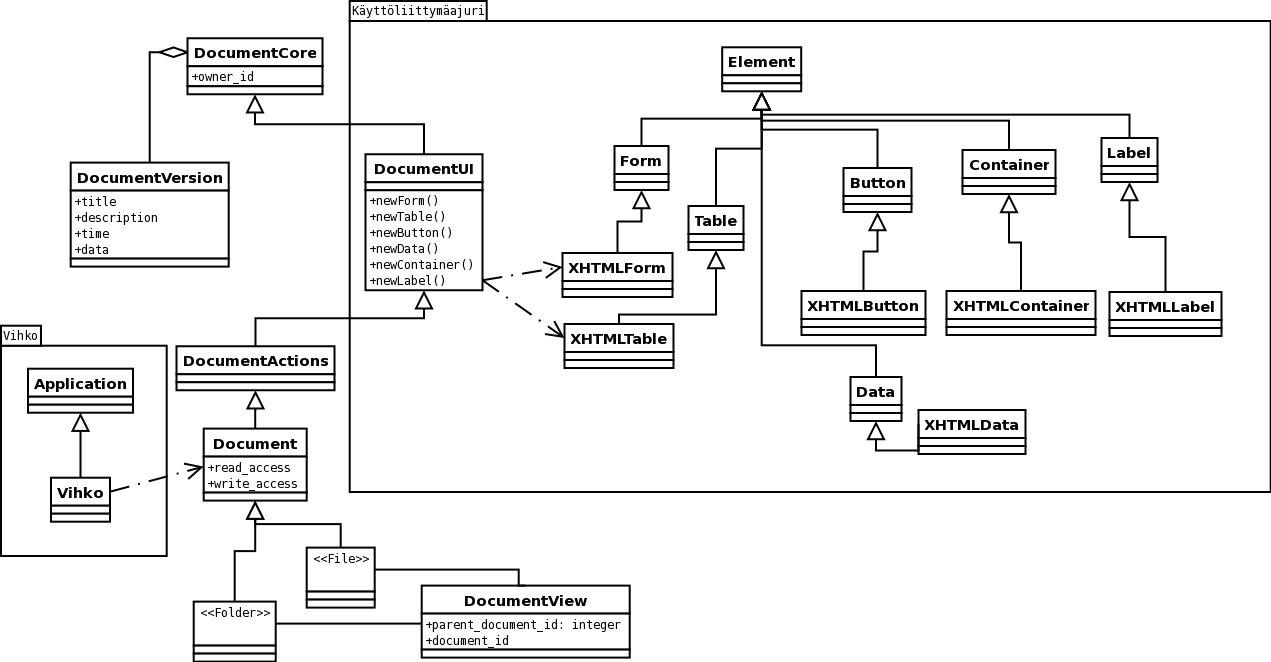
\includegraphics[width=\linewidth]{kuvat/oppimappi-schema-current}
\caption{Osa toteutetusta Oppimapin rakenteesta}
\label{fig:oppimappi-schema-current}
\end{kuva}

K�yt�nn�ss� k�ytt�liittym�st� vastaavan kerroksen pilkkominen osiin
selaimen sek� palvelimen vastuulle aiheutti sen, ett�
k�ytt�liittym�ajurin piti ymm�rt�� enemm�n selaimen toiminnasta.  T�m�n
seurauksena arvioin, ett� helpoin ratkaisumalli olisi kehitt��
sovelluskehys Oppimapin kehitt�miseksi. Tulevaisuudessa, kun Oppimapin
lis�ksi tehd��n uusia ty�kaluja, voidaan sovelluskehys k�ytt��
uudelleen. My�s lokalisointiin tarvittava logiikka on yhteinen eri
sovellusten v�lill�. Itse Oppimappi on vain eri tiedostotyyppej�
toteuttavien moduulien ohjelmakoodi itse sovelluskehyksen rinnalla.
T�ll� hetkell� vaikuttaa lis�ksi silt�, ett� suurin osa Peda.netin
tulevista sovelluksista voidaan kirjoittaa Oppimapin moduuleiksi sen
sijaan, ett� niist� teht�isiin omia, samaa sovelluskehyst� k�ytt�vi�
sovelluksia. Oppimapista voidaan my�s tarvittaessa rakentaa muita
toimintaymp�rist�j� j�tt�m�ll� osa k�yt�ss� olevista moduuleista pois
tai korvaamalla niit� uusilla.

\subsection{Tiedon siirto lomakkeiden v�lill�}

Kaikki Oppimapin moduulit perit��n luokasta \class{Document} (ks. kuva
\ref{fig:oppimappi-schema-current}) ja kaikki moduulit saavat oman
nimiavaruuden k�ytt�milleen parametreille. T�m� on olennaista, koska
istuntoon liittyv�� tietoa t�ytyy kuljettaa kaikkien linkkien
osoitteissa, kuten luvussa \ref{kaikki-data-sivulla} selitin. Eri
moduulien parametrit sijoitetaan puolestaan omiin nimiavaruuksiinsa,
jotta useita moduuleita olisi mahdollista esitt�� rinnakkain samalla
sivulla. Automaattinen parametrien uudelleennime�minen mahdollistaa
my�s sen, ettei yksitt�ist� moduulia ohjelmoitaessa tarvitse
tarkistaa mit� nimi� muut moduulit k�ytt�v�t.

Esimerkiksi jos moduuli, jonka id"-numero on \code{251} asettaa sivulle
parametrin, jonka nimi on \code{foo}, k�ytet��n todellisena parametrin
nimen� merkkijonoa \code{p251xfoo}. Nimen muunnos tapahtuu
automaattisesti luokan \class{DocumentUI} toimesta.  Lis�ksi
\class{DocumentUI}"-luokka yll�pit�� automaattisesti istuntotietoa.
T�m� toteutetaan globaalin \code{session}"-parametrin avulla, joka
sis�lt�� k�ytt�j�n ja tietokannan tunnistetiedot sek� varmenteen
tietojen muuttumattomuudesta. Kaikkiin toimintoihin lis�t��n my�s
kullakin hetkell� k�yt�ss� olevan moduulin tunniste sek� edellisen
k�yt�ss� olleen moduulin tunniste. N�iden tietojen avulla moduulin
kaikista toiminnoista palataan oletuksena takaisin samaan moduuliin,
mutta esimerkiksi \emph{tallenna}"-toiminnon j�lkeen voidaan palata
edelliseen moduuliin. T�m�n voi ajatella vastaavan tavallisessa
k�ytt�j�rjestelm�ss� ikkunan sulkemista, jonka j�lkeen aktiiviseksi
vaihtuisi edellinen ikkuna.

Oppimappi erottelee istuntoon liittyv�n tiedon kahteen eri ryhm��n:
ikkunakohtaiset tiedot ja yleiset asetukset. Kaikki yleiset asetukset
tallennetaan palvelimen tietokantaan ja ne haetaan tietokannasta
jokaisen sivun generoinnin alussa. Tietojen hakeminen aina jokaisen
sivun alussa lis�� palvelimen kuormaa hieman, mutta se mahdollistaa
kuorman jakamisen eri edustakoneiden kesken, sill� Oppimappia ajava
edustakone ei tallenna mit��n tietoja k�ytt�j�st�. Asetukset ja tiedot,
jotka ovat aikaan sidottuja ja joiden vaikutuksen pit�� n�ky� selaimen
historia"-toimintoja k�ytett�ess� tallennetaan jokaiseen sivuun
upotettuna. T�ll� hetkell� ne koodataan kaikkiin linkkeihin, mutta
tulevaisuudessa ne olisi mahdollista sijoittaa sivun sijainnin
osoittavaan polkuun. Koska HTML"-standardi m��rittelee suhteellisen viittauksen mahdollisuuden linkeiss�, voisi Oppimappi sijoittaa kaikki sivukohtaiset tiedot sivun osoitteeseen.

Esimerkiksi osoitteessa
\code{http://peda.net/mappi""?session=databasetest/""1/""9325""35/""53""252""\&=4""/6""/1}
oleva Oppimapin dokumentti voitaisiin siirt�� osoitteeseen 
\code{http://""peda.""net/""mappi/""databasetest.""1.""932535.""53252/""4.""6.""1},
jolloin uuteen sivuun viitatessa ei tarvisisi toistaa en�� istuntoon
liittyv�� tietoa vaan ainoastaan sivukohtaiset muutokset. T�ll�in
esimerkiksi linkki \verb!<a href="?x=y">linkkiteksti</a>! osoittaisi
automaattisesti samaan istuntoon ja samaan dokumenttiin ja selain
l�hett�isi linkin mukana parametrin $x$ arvolla ``y''. Nykyisin
kaikissa linkeiss� pit�� aina toistaa parametrit \code{session} ja
\code{d}.

Koska kaikki n�m� tiedot vied��n jokaiseen sivuun upotettuna, toimii
edelliseen n�kym��n palaaminen my�s historian kautta avatuissa sivuissa
oikein. My�sk��n ikkunan kahdentaminen ei aiheuta ongelmia.
Kirjanmerkkien k�ytt� toimii lukuunottamatta sit�, ett� tietoturvan
lis��miseksi annetut linkit vanhenevat tunnin kuluessa -- kirjanmerkki�
voidaan k�ytt�� t�m�nkin j�lkeen, mutta sit� k�ytett�ess�
k�ytt�j�tunnus ja salasana kysyt��n ensin uudelleen.


\chapter{Peda.net "=hanke}

\begin{chapterquote}{Lainaus esiselvityksen johdannosta} Koulutus on
investointi tulevaisuuteen. T�m�n p�iv�n ratkaisut vaikuttavat
\mbox{10--20} vuoden aikaj�nteell� ty�el�m��n ja muuhun yhteiskuntaan viel�
\mbox{30--40} vuoden kuluttua. Toisaalta tulevaisuus, johon koulutuksen tulisi
lapsia ja nuoria valmentaa, on yh� nopeammin muuttuva ja vain lyhyell�
aikav�lill� ennakoitavissa. \end{chapterquote}

Peda.net\footnote{Peda.net on Jyv�skyl�n yliopiston rekister�ity
tavaramerkki.} sai alkunsa Jyv�skyl�n Yliopiston tekem�st�
telemaattisen opetusverkon hy�dynt�mismahdollisuuksien esiselvityksest�
vuonna 1996. Esiselvityksess� tutkittiin mahdollisuuksista luoda uusia
oppimisymp�rist�j� eri Keski"-Suomen kouluasteille. Esiselvitys
perusteli uusien ymp�rist�jen tarvetta seuraavasti:

\begin{quote} Oppiminen perustuu olemassa olevan tiet�myksen
jalostamiseen. Yksitt�isten tietojen ulkokohtainen muistaminen ei
edist� taitoa k�ytt�� tiet�myst��n itsen�isesti ja luovasti. Uusi
oppimisymp�rist� edellytt�� mahdollisuutta k�ytt�� monipuolisia
tietol�hteit� oma"-aloitteisesti. T�ss� tietoteknologia tarjoaa kaikille
kouluille ja jokaiselle oppilaalle aivan uudenlaisen mahdollisuuden
tiedon hankintaan ja kokemusten vaihtamiseen. \end{quote}

Esiselvityksen suosittelema PEDANET"-hanke k�ynnistyi vuonna 1997
Keski"-Suomen kuntien yhteisty�n�. Hankkeen ensimm�isen vaiheen
rahoitus jaettiin Keski"-Suomen liiton verkottumiseen varatuista
EU-tuista. K�yt�nn�ss� hankkeen k�yt�nn�n toteutus oli hyvin kaukana
esiselvityksen sis�ll�st�, joka sis�lsi suunnitelman esimerkiksi
PEDANET"-hankkeen hallinnoimasta kouluverkosta. Eli PEDANET olisi
t�ll�isen tavoitteen mukaisesti vastannut koulujen internet-yhteyksien
yll�pit�misest�. My�hemmin todettiin, ett� t�ll�inen teht�v� ei vastaa
yliopiston tavoitteita. \cite{pedanet:esiselvitys}

Hanke on toiminut alusta asti Jyv�skyl�n Yliopiston Koulutuksen
tutkimuslaitoksen (\alt{KTL}) alaisuudessa, jossa taustahenkil�n� on
ollut laitoksen nykyinen johtaja Jouni V�lij�rvi. Teknisen�
vastuuhenkil�n� toimi aluksi Jari Hautam�ki, joka oli ottanut teht�v��
varten virkavapaata normaalista ty�st��n Jyv�skyl�n teknillisen
oppilaitoksen opettajana. Hautam�ki otti ty�h�n avukseen silloisen
oppilaansa Juha Lahden, joka on jatkanut hankkeen ty�ntekij�n� t�h�n
p�iv��n asti.

\section{Pedanet vaihe I, 1997--1999}

Pedanet"-hanke k�ynnistyi Keski"-Suomen liiton, Jyv�skyl�n yliopiston,
Jyv�skyl�n ammattikorkeakoulun ja Telecom Finland Oy eli Telen v�lisen
aiesopimuksen allekirjoittamisella vuonna 1997. Aiesopimuksen mukaan
Pedanet tulisi muodostumaan kahdesta itsen�isest� osasta: oppilaitosten
v�lisest� verkosta sek� tietoverkkoon pohjautuvasta opetuksen
kehitt�misest�. \cite{pedanet:aiesopimus}.

Oppilaitosten v�lisen verkon yll�pito ja kehitt�minen j�i osin
toteutumatta ja Pedanet olikin mukana vain koordinoimassa Keski"-Suomen
koulujen verkottumista, mutta rahoituksen ja k�yt�nn�n j�rjestelyt
j�senkunnat hoitivat t�lt� osin itse. K�yt�nn�ss� Pedanetin ensimm�inen
vaihe muodostui kymmenest� pilottiprojektista
\cite{julkaisematon-pedanet-pilottisuunnitelma}. Maininnan arvoisesti
kaikki oppinaineiden sis�ll�ntuotantoon liittyneet projektit j�iv�t
pilottiprojektin tasolle. Vaikutti silt�, ett� opettajat eiv�t ehdi
varsinaisen kouluty�n sivussa tuottaa oppimateriaalia, mutta muiden
pilottien perusteella opettajat olivat kiinnostuneet olemassaolevan
materiaalin tarjolleasettamisesta verkkoon. Kymmenest� pilotista
pitk�aikaisemmiksi j�i vain nelj�:

\begin{description}

\item[Kyl�koulujen verkottuminen ja opetuksen monipuolistaminen,] jonka
tavoitteena oli edist�� haja-asutusalueiden pienten ala-asteen koulujen
edellytyksi� hy�dynt�� tietoverkkoja opetuksessa toimimalla
yhteisty�ss� kesken��n. T�ss� pilotissa olivat mukana muun muassa
Kekkil�n, Saarij�rven, Toivakan ja Joutsan koulut.

\item[Koulun Online "-ymp�rist�n luominen,] jonka tavoitteena oli luoda
uusi internetin v�lityksell� toimiva online-palvelu, johon voidaaan
liitt�� koulun ja sen eri toiminnallisten ryhmien (luokat, opettajat,
henkil�kunta) tavoitteiden mukainen toiminta. T�ss� pilotissa olivat
mukana Vitikkalan ala-aste ja J�ms�n koulu.

\item[Verkostokoulu valinnaisuuden monipuolistajana,] jonka tavoitteena
oli lis�t� valinnaisuutta pohjoisen Keski"-Suomen oppilaitokseissa
tarjoamalla niille opetusta ja sis�lt�j� yhteisen tietoverkon kautta.
T�ss� pilotissa olivat mukana kaikki pohjoisen Keski"-Suomen
oppilaitokset.

\item[Koulutustasojen yhteisty� -- p�iv�kodista kouluun,] jossa
tutkittiin p�iv�kodin ja peruskoulun v�lisen yhteisty�n
toteuttamistapoja. Tietoverkkoja pyrittiin k�ytt�m��n opettajien
ammmatillisen keskustelun ja asiantuntijuuden edist�miseksi, sek�
lasten kokemusten v�litt�misess� digitaalisia portfolioita hy�dynt�en.

\end{description}

Yhteisen� nimitt�j�n� n�ill� piloteilla oli ``Online''"-nimell�
kulkeneen verkkojulkaisuv�lineen k�ytt�. Juha Lahti r��t�l�i siit�
paremmin pienille lapsille soveltuvan version. Online
verkkojulkaisuv�lineen nimeksi tuli my�hemmin Verkkolehti, jonka uusin
versio on nykyisin Pedanetin toiseksi k�ytetyin ty�kalu.

Ty�kalujen merkitys johtuu todenn�k�isesti siit�, ett� koulujen
verkottuminen oli p��asiassa seurausta Opetushallituksen
Tietosuomi"-hankeen tavoitteista. Opetushallitus pyrki kannustamaan
opettajia hankkimaan tarvittavia taitoja tietoverkon k�ytt�miseen
opetuksessa. K�yt�nn�ss� tuohon aikaan tiedon julkaiseminen verkossa
vaati paljon teknist� ymm�rryst� ja Pedanetin helppok�ytt�iset ty�kalut
antoivat mahdollisuuden tuottaa sis�lt�� verkkoon ymm�rt�m�tt� teknisi�
yksityiskohtia. Paljon merkityst� on ollut ilmeisesti my�s sill�, ett�
Pedanetin ohjelmat ovat aina toimineet hankkeen palvelimilla, joten
koulujen ei ole tarvinnut asentaa niit� varten erillisi� sovelluksia. 
Varsinkin pienemmiss� kouluissa atk-j�rjestelyist� vastaa usein
matematiikan tai fysiikan opettaja, joten aikaa suuriin
ohjelmistoasennuksiin ei yleens� ole.

Projektissa ty�skenteliv�t p��asiassa Juha Lahti tekniikasta vastaavana
henkil�n�, joka my�s toteuttu palvelinsovellusten ohjelmointia ja
toimintaa koordinoi Pentti Pirhonen, joka oli virkavapalla J�ms�n
lukion rehtorin toimesta. Itse toimin ensimm�isen vaiheen aikana
hankkeessa p�tk�t�iss� asevelvollisuuden suorittamisen j�lkeen vuonna
1998. Teht�viini kuului www"-sivuston yll�pitoa ja
palvelinohjelmistojen kehitt�mist�. Pedanetin levitt�misest� vastasi
t�h�n aikaa p��asiassa T�ydennyskoulutuskeskus, joka koulutti
Pedanet-ty�v�lineiden k�ytt��.

Ensimm�isen vaiheen aikana nimi Pedanet vaihtui ep�virallisesti
Peda.netiksi ja internet"-osoite muuttui sijainnista
\url{http://pedanet.jyu.fi/} osoitteeseen \url{http://peda.net/}, jossa
se nykyisinkin toimii.

\subsection{Peda.netin ensimm�isen vaiheen sovellustuotantoa}

Kuten yll� mainitsin, Juha Lahden Online"-ymp�rist� oli merkitt�v�ss�
roolissa onnistuneissa pilottiprojekteissa. T�m� aluksi Online"-nimell�
kulkenut ymp�rist� nimettiin my�hemmin Verkkolehdeksi ja sen
versiohistoria on seuraava:

\begin{ol}

\item Juha sai kopion Vitikkalan ala-asteen k�ytt�m�n verkkoymp�rist�n
l�hdekoodista 1998 (XXX:lta???) ja h�n lis�si siihen tiedostojen
l�hett�mistoiminnon (\alt{file upload}), joka oli uusimpien
www"-selainten uusi ominaisuus. T�m� oli ensimm�inen Pedanetin tarjoama
ty�v�line, jota muutama koulu k�ytti. Teknisesti ty�kalu oli toteutettu
Perl-ohjelmointikielell� ja muutokset tehtiin suoraan
tiedostoj�rjestelm��n.

\item My�hemmin samana vuonna Juha uudelleenkirjoitti verkkolehden
ohjelmakoodin helpommin yll�pidett�v��n muotoon. Toiminnallisia
ongelmia korjattiin.

\item Verkkolehdest� tehtiin kolmas versio vuonna 1999, jossa tiedot
tallennettiin SQL"-tietokantaan. J�rjestelm� toimi
Perl-ohjelmointikielell� ja tietokannan teht�v�� hoiti miniSQL.

\end{ol}
Verkkolehden lis�ksi oli k�yt�ss� Jyv�skyl�n yliopistolla Cum Laude
"-ty�projektina toteutettu OPSpro-sovellus. Osa Keski"-Suomen koulusta
k�ytti my�s 1999 kirjoittamaani Kurssitarjotin"-sovellusta. Pedanetin
toiminnassa oli jo tuolloin havaittavissa nopea ohjelmistonkehityksen
tahti; olennaista oli saada jotakin valmiiksi ja palautetta k�ytt�jilt�
-- t�ss� tapauksessa opettajilta.


\section{Pedanet vaihe II, 2000--2001}

Pedanet"-hankkeen ensimm�isen vaiheen rahoitus kesti vuoden 1999
loppuun asti. KTL haki 1999 rahoitusta Pedanet-hankkeen toista vaihetta
varten. Hankesuunnitelman perusteluissa luki muun muassa:

\begin{quote} Syntyneiden palveluiden laajamittainen k�ytt��notto ja
edelleen kehitt�minen voidaan parhaiten turvata vuosille 2000--2001
ajoittuvalla uudella hankkeella, joka uuden valtakunnallisen
tietoyhteiskuntastrategian mukaisesti profioidaan selv�sti verkon
sis�lt�jen ja palvelujen kehitt�mishankkeeksi. \end{quote}

Hankesuunnitelman 12 osaprojektista vain muutama jatkoi toisen vaiheen
rahoituksen loppumisen j�lkeen:

\begin{description}

\item[Liikennekasvatuksen verkkopalvelu liikenne.peda.net,] jonka
tavoitteena oli luoda yhteisty�ss� Liikenneturvan kanssa koulujen
liikenneasvatusta tukeva verkkopalvelu. Sivuston yll�pito on jatkunut t�h�n p�iv��n saakka.

\item[Oppiaineiden verkkoymp�rist�t,] jonka tavoitteena oli kehitt��
opettajien tarpeisiin oppiainekohtaisia ty�kaluja syyskuussa 1999
l�hetetyn kyselyn perusteella. K�yt�nn�ss� palautteen perusteella
kehitettiin Verkkover�j�n olemassaolevia moduuleita tai luotiin uusia, paremmin tarpeeseen sopivia.

\item[Verkkotiedottamisj�rjestelmien kehitt�minen erilaisiin
koulutoimen tarpeisiin,] jonka tavoitteena oli kartoittaa koulutoimen
tiedottamistarpeet ja tarjota verkkotiedottamisymp�rist�j�. K�yt�nn�ss�
tiedotus hoidettiin Verkkover�j�n moduulien avulla. My�s Verkkolehte� k�ytettiin joissakin kouluissa.

\item[EU"-koulutusohjelmien verkkopalveluiden kehitt�minen,] jonka
keskeisen� osana oli tukea Sokrates"-koulutusohjelman eri osioissa
mukana olevia kouluja. Koska koulut sijaitsivat maantieteellisesti
kaukana toisistaan eiv�t oppilaat voineet n�hd� toisiaan kasvotusten
vaan kommunikointi tapahtui oppimisymp�rist�jen kautta. K�yt�nn�ss�
verkkolehdest� tehtiin t�m�n projektin puitteissa englanninkielinen
versio projektin tarpeisiin.


\item[Keski"-Suomen kouluverkon laajakaistainfrastruktuurin kehitys],
joka k�yt�nn�ss� koordinoi kuntien verkottumishankkeita. Pedanet auttoi
muun muassa rahoituksen hakemisessa Opetushallitukselta ja tiedotti eri
rahoitusvaihtoehdoista. Pedanet ei sin�ns� toteuttanut yhteyksien
rakentamista.

\end{description}

\subsection{Peda.netin toisen vaiheen sovellustuotantoa}

Hankkeen toisen vaiheen aikana kehitettiin kouluille useita uusia
sovelluksia. My�s aikaisemmin k�yt�ss� olleita ty�kaluja, Verkkolehte�
ja OPSpro"-sovellusta p�ivitettiin. Verkkolehden vuoden 2000 lopussa
valmistunut nelj�s versio, josta k�ytt�j�t edelleen k�yttiv�t vain
nimityst� ``Verkkolehti'', oli itse asiassa Juha Lahden opinn�ytety�.
T�m� verkkolehden versio pysyikin k�yt�ss� Verkkolehden viidenteen,
vuonna 2004 julkaistuun versioon -- t�ll� kertaa virallisesti
``Verkkolehti 2'' -- saakka.

Toisen vaiheen aikana kehitin itse OPSpro"-sovelluksen toisen version,
joka olikin hetken ajan k�yt�ss�, mutta koulut eiv�t ilmeisesti olleet
viel� valmiita er�isiin sen ominaisuuksiin: erityisesti k�ytt�jien
hallinta tuotti ongelmia. Muissa ty�kaluissa oli tuohon aikaan
yll�pitoon vain yksi salasana koulua kohden ja t�h�n verrattuna usean
k�ytt�j�tunnuksen yll�pito oli liian vaativaa. Samoin rakenteisen
dokumentin kappaleiden oikeuksien hallinta osoittautui liian vaikeaksi.
OPSpro2-sovelluksen j�lkeen tein ensimm�isen version Verkkover�j�st�
vuonna 2001.

Juha teki viel� OSPpro-sovelluksesta syksyll� 2001 Verkkolehden
ohjelmakoodin pohjalta yksinkertaisemman version. T�m� OPSpro-version
on viel� nykyisinkin k�yt�ss�.

%ver�j�n v3 (virallisesti "2") kes�-joulu 2003 (php, mysql)

%verkkolehti 5 (virallisesti "2"), 2004

%sosiaalinen innovaatio

% Omat softat:
% Toisen asteen kurssitarjotin (1999)
% OPSpro2 (2000)
% Verkkover�j� (ty�nimi: Portaali, 2001)
% Verkkover�j� 2 (ty�nimi: Portal2, 2002)
% YALE2 eli \alt{Yet Another Learning Environment 2} (2003)
% Oppimappi (ty�nimi: Vihko, 2003--2004)

\section{Hankkeen rahoitus loppui, uusi toimintamalli edess�}

Pedanet"-hankkeen toinen vaihe p��ttyi vuoden 2001 lopussa ja muuttui
silloin Jyv�skyl�n yliopiston Koulutuksen tutkimuslaitoksen
koordinoimaksi tutkimus- ja kehitt�mishankkeeksi -- nyt nimen� oli jo
virallisestikin Peda.net. T�st� eteenp�in Peda.net on toiminut
omarahoitteisena j�senilt� ker�ttyjen vuosimaksujen turvin.

Peda.net"-kouluverkon j�senet saavat vuosittaisen j�senmaksun
vastineena vapaan k�ytt�oikeuden kaikkiin Peda.netin kehitt�miin ja
yll�pit�miin sovelluksiin ja p��sev�t halutessaan osallistumaan uusien
sovellusten kehitt�miseen. Peda.netill� oli vuoden 2004 tammikuussa
j�senin� 70 kuntaa (j�senkunnan kaikilla kouluilla on vapaa
k�ytt�oikeus kaikkiin Peda.net"-verkkoty�v�lineisiin) ja sen lis�ksi
yksitt�isi� kouluja tai oppilaitoksia oli yli 50 kunnassa. Toiminta on
voittoa tavoittelematonta.

\section{Tutkimusty�}

Peda.net"-kouluverkko toimii Koulutuksen tutkimuslaitoksessa Tietoverkot
oppimis- ja ty�ymp�rist�iss� "=tutkimusryhm�n yhteydess�. Tutkimusryhm�n
tavoitteena on tarkastella teknologian ja virtuaalisten
oppimisymp�rist�jen mahdollisuuksia oppimisen ja opetuksen tukena.
Tutkimusryhm�n tekem� tutkimus on yht��lt� monitieteist�,
teoreettisesti painottunutta perustutkimusta sek� toisaalta
k�yt�nn�llist� l�ht�kohdista nousevaa kehitt�mistutkimusta.

Peda.net kouluverkkoon liittyv� tutkimus on kehitt�mistutkimusta, joka
tapahtuu l�heisess� yhteisty�ss� koulujen ja opettajien kanssa. Eri
oppilaitosten ja organisaatioiden henkil�st�n lis�ksi
tutkimusyhteisty�ss� on mukana my�s muita alan kansallisia ja
kansainv�lisi� asiantutkijoita.

\section{Kokonaiskuva nykytilanteesta}

Hankkeessa ty�skentelee nykyisin kolme t�ysip�iv�ist� ty�ntekij��:
Jaana Kettunen, Juha Lahti ja Jarkko Lampinen. Kirjoittaja toimii
nelj�nten� ty�ntekij�n� puolip�iv�isen�. Kaikki Peda.netin palvelut
py�riv�t nelj�ll� Koulutuksen tutkimuslaitoksen kellarissa py�riv�ll�
Linux"-palvelimella.


\section{Peda.netiss� kirjoittajan kehitt�mi� sovelluksia ja
prototyyppej�}

Kuten aikaisemmin mainitsin, olen ty�skennellyt Peda.netiss� syksyst�
1998 alkaen, joten kokemusta erilaisista selaink�ytt�isist�
sovelluksista on kertynyt jo useammalta vuodelta. K�sittelen
seuraavassa kehitt�m�ni sovellukset aikaj�rjestyksess�.

\subsection{Toisen asteen kurssitarjotin}

Toisen asteen kurssitarjotin kehitettiin Peda.netin toimesta kes�ll�
1999, Jyv�skyl�n Ammattioppilaitoksen (nykyinen \alt{Jyv�skyl�n
ammattikorkeakoulu}) ja sen kanssa yhteisty�ss� toimivien koulujen
k�ytt��n. Sovelluksen kehitt�mist� koordinoi Peda.netin puolesta Pentti
Pirhonen ja kurssitarjottimen k�ytt�ji� edusti Vuokko Pennanen.

Sovelluksen taustalla oli samalla nimell� tuotettu paperiversio eri
oppilaitosten j�rjest�mist� kursseista. Tavoitteena oli j�rjest�� eri
oppilaitoksissa (k�yt�nn�ss� ammattikouluissa ja lukioissa) kursseja,
joille muiden oppilaitosten oppilaat saattoivat osallistua. Toisen
asteen kurssitarjotin sis�lsi samat tiedot kuin paperiopaskin. Lis�ksi
siin� oli yll�pitok�ytt�liittym� uusien kurssien, koulujen ja
opettajien sy�tt�miseen, muokkaamiseen ja poistamiseen, sek�
ilmoittautumisj�rjestelm� eri kursseille hakemiseksi.

Teknisesti Toisen asteen kurssitarjotin py�ri Linux"-palvelimella
Perl"-ohjelmointikielell� toteutettuna. Tietokannan teht�v�� hoiti
miniSQL"-ohjelmisto samalla koneella. Kun ottaa huomioon, etten ollut
t�t� sovellusta ennen tehnyt edes yksinkertaista CGI"-sovellusta,
t�ytyy olla tyytyv�inen lopputulokseen. Ohjelman perusrakenne perustui
osin Verkkolehden vuonna 1999 tehtyyn versioon.

Kurssitarjotin kehitettiin siihen aikaa yleiseen (selaink�ytt�isten
sovellusten) tyyliin, jossa ohjelman toiminta ja k�ytt�liittym�n
toimintaan liittyv� koodi oli sidottu melko tiukasti toisiinsa. Lis�ksi
normaali tietojen selailu "=k�ytt�liittym� ja yll�pitok�ytt�liittym�
toimivat omina sovelluksinaan k�ytt�en yhteist� tietokantaa. Ohjelman
yll�pito todettiin hankalaksi ohjelman heikon rakenteen,
miniSQL"-tietokannan rajoittuneisuuden ja kokonaisuuden sirpaleisuuden
vuoksi (selailu ja yll�pito k�yttiv�t osittain poikkeavia
k�ytt�liittymi�, mik� puolestaan koettiin huonona k�ytett�vyyten� --
t�m�n korjaaminen taas oli ty�l�st� ohjelman huonohkon teknisen
rakenteen seurauksena). Sovellukseen tehtiin pieni� korjauksia syksyll�
2000, ja silloin virallinen nimi oli ``Toisen asteen yhteys'' ja
yhteyshenkil�ksi oli vaihtunut Taina Roivainen. Uutta, t�ysin korjattua
versiota ei alettu koskaan tekem��n, vaan seuraavana projektina
siirryin kehitt�m��n OPSpron uutta versiota. Kurssitarjottimen k�ytt�
loppui kes�ll� 2001.

\subsection{OPSpro2"-prototyyppi}

\begin{quote} Opetussuunnitelman kehitt�misen eli OPS"-ty�n tulisi olla
koulussa jatkuva, p�ivittyv� prosessi. OPSpro on helppok�ytt�inen
ty�v�line opetussuunnitelman tekemiseen, yll�pit�miseen ja
julkaisemiseen. Ty�v�line mahdollistaa mm. asiantuntijoiden ja
vanhempien osallistumisen sek� hallinnon lomakkeiden ja asiakirjojen
jakamisen. OPSprossa voit helposti monipuolistaa ulkoasua ja sis�lt��
kuvilla sek� ��ni- ja videoleikkeill�. \\
\mbox{}\hfill\mbox{---~\emph{OPSpro"-esittely}} \end{quote}

OPSpro eli opetussuunnitelmaprosessori, on hajautettu, rakenteisen
dokumentin tuottamissovellus. Koska jokaisella koululla tulee olla oma,
yksil�llinen opetussuunnitelma, ja toisaalta opetussuunnitelman
jokainen osa on parhaimmillaan t�ysin erillinen osuus (esimerkiksi
kuvaus englanninkielen opetuksesta yl�asteella) voi dokumentin eri osia
kirjoittaa samanaikaisesti useat eri henkil�t. OPSpron avulla
esimerkiksi �idinkielen opettaja voi kirjoittaa ja yll�pit��
opetussuunnitelman �idinkielen osuutta samaan aikaan, kun matematiikan
opettaja vastaavasti yll�pit�� omaa osuuttaan. OPSpro huolehtii
automaattisesti rakenteen yll�pit�misest� (eli �idinkieli ja englanti
ovat koko opintosuunnitelman alilukuja) ja koko dokumentin
kokoamisesta. T�ll�in dokumentin eri osia ei tarvitse l�hett��
esimerkiksi s�hk�postilla koko dokumentin kokoamisesta vastaavalle
henkil�lle, joka koostaisi koko dokumentin esimerkiksi MS Word
"=tekstink�sittelyohjelmalla. Ohjelman nykyisin k�yt�ss� olevalla
versiolla on kirjoitettu ongelmitta yli 500 sivun dokumentteja.

OPSpro ei sin�ns� pakota juuri opetussuunnitelman tekemiseen, vaikka
osa k�ytt�liittym�ss� k�ytetyist� termeist� siihen suuntaan viittaakin.
Kyseess� on pikemminkin yhteisty�ss� tuotettavien rakenteisten
dokumenttien kirjoittamiseen suunniteltu ty�kalu.

\subsection{OPSpro-sovelluksen kehityskaari}

Ensimm�inen OPSpro kehitettiin 1999 Jyv�skyl�n yliopiston
tietotekniikan laitoksen Cum Laude "=ty�projektina. T�m�n sovelluksen
tekninen toteutus todettiin kuitenkin my�hemmin selv�sti
riitt�m�tt�m�ksi. Kirjoittajan teht�v�ksi j�i kehitt�� samaan ideaan
perustuen parempi versio kes�ll� 2000. T�m� versio j�i loppujen lopuksi
prototyypiksi. Suurimmat syyt olivat teknisi�: ohjelma toteutettiin
Perl"-ohjelmointikielell� miniSQL"-tietokannan p��lle.
MiniSQL"-tietokannan nopeus ja vakaus tekiv�t siit� teknisesti huonon
alustan. Lis�ksi Peda.netin kaikki ty�kalut on sittemmin p��tetty
toteuttaa PHP"-ohjelmointikielell� yll�pidon ja integroinnin
helpottamiseksi.

Toiminnallisesti sovellus pystyi tekem��n suuren osan siit�, mit�
nykyinenkin versio. Se tarjosi jopa enemm�n mahdollisuuksia k�ytt�j�n
suorittamaan r��t�l�intiin koulukohtaisesti, erityisesti
k�ytt�liittym�n osalta. K�yt�nn�ss� k�ytt�liittym�n r��t�l�inti
osoittautui liian vaikeaksi tavalliselle opettajalle tai koulun
atk"-yll�pit�j�lle (joka yleens� on todellisuudessa matematiikan tai
tietotekniikan opettaja). Lis�ksi havaittiin, ett� Peda.netin
k�ytt�jille t�rke�mp�� oli helppo k�ytett�vyys kuin sovelluksen hieno
ulkon�k� -- kaikki k�ytt�j�t tyytyiv�t poikkeuksetta oletusulkon�k��n.

Nykyisin k�yt�ss� oleva OPSpron versio on Juha Lahden
PHP"-ohjelmointikielell� ohjelmoima ja se toimii
MySQL"-tietokantaohjelmistolla. Sovelluksen ohjelmakoodi on osin sama
Verkkolehden aikaisemman version kanssa. Tammikuussa 2004 sovelluksella
toimitettuja opetussuunnitelmia oli noin 600.

\subsection{Verkkover�j�}

\begin{kuva}
%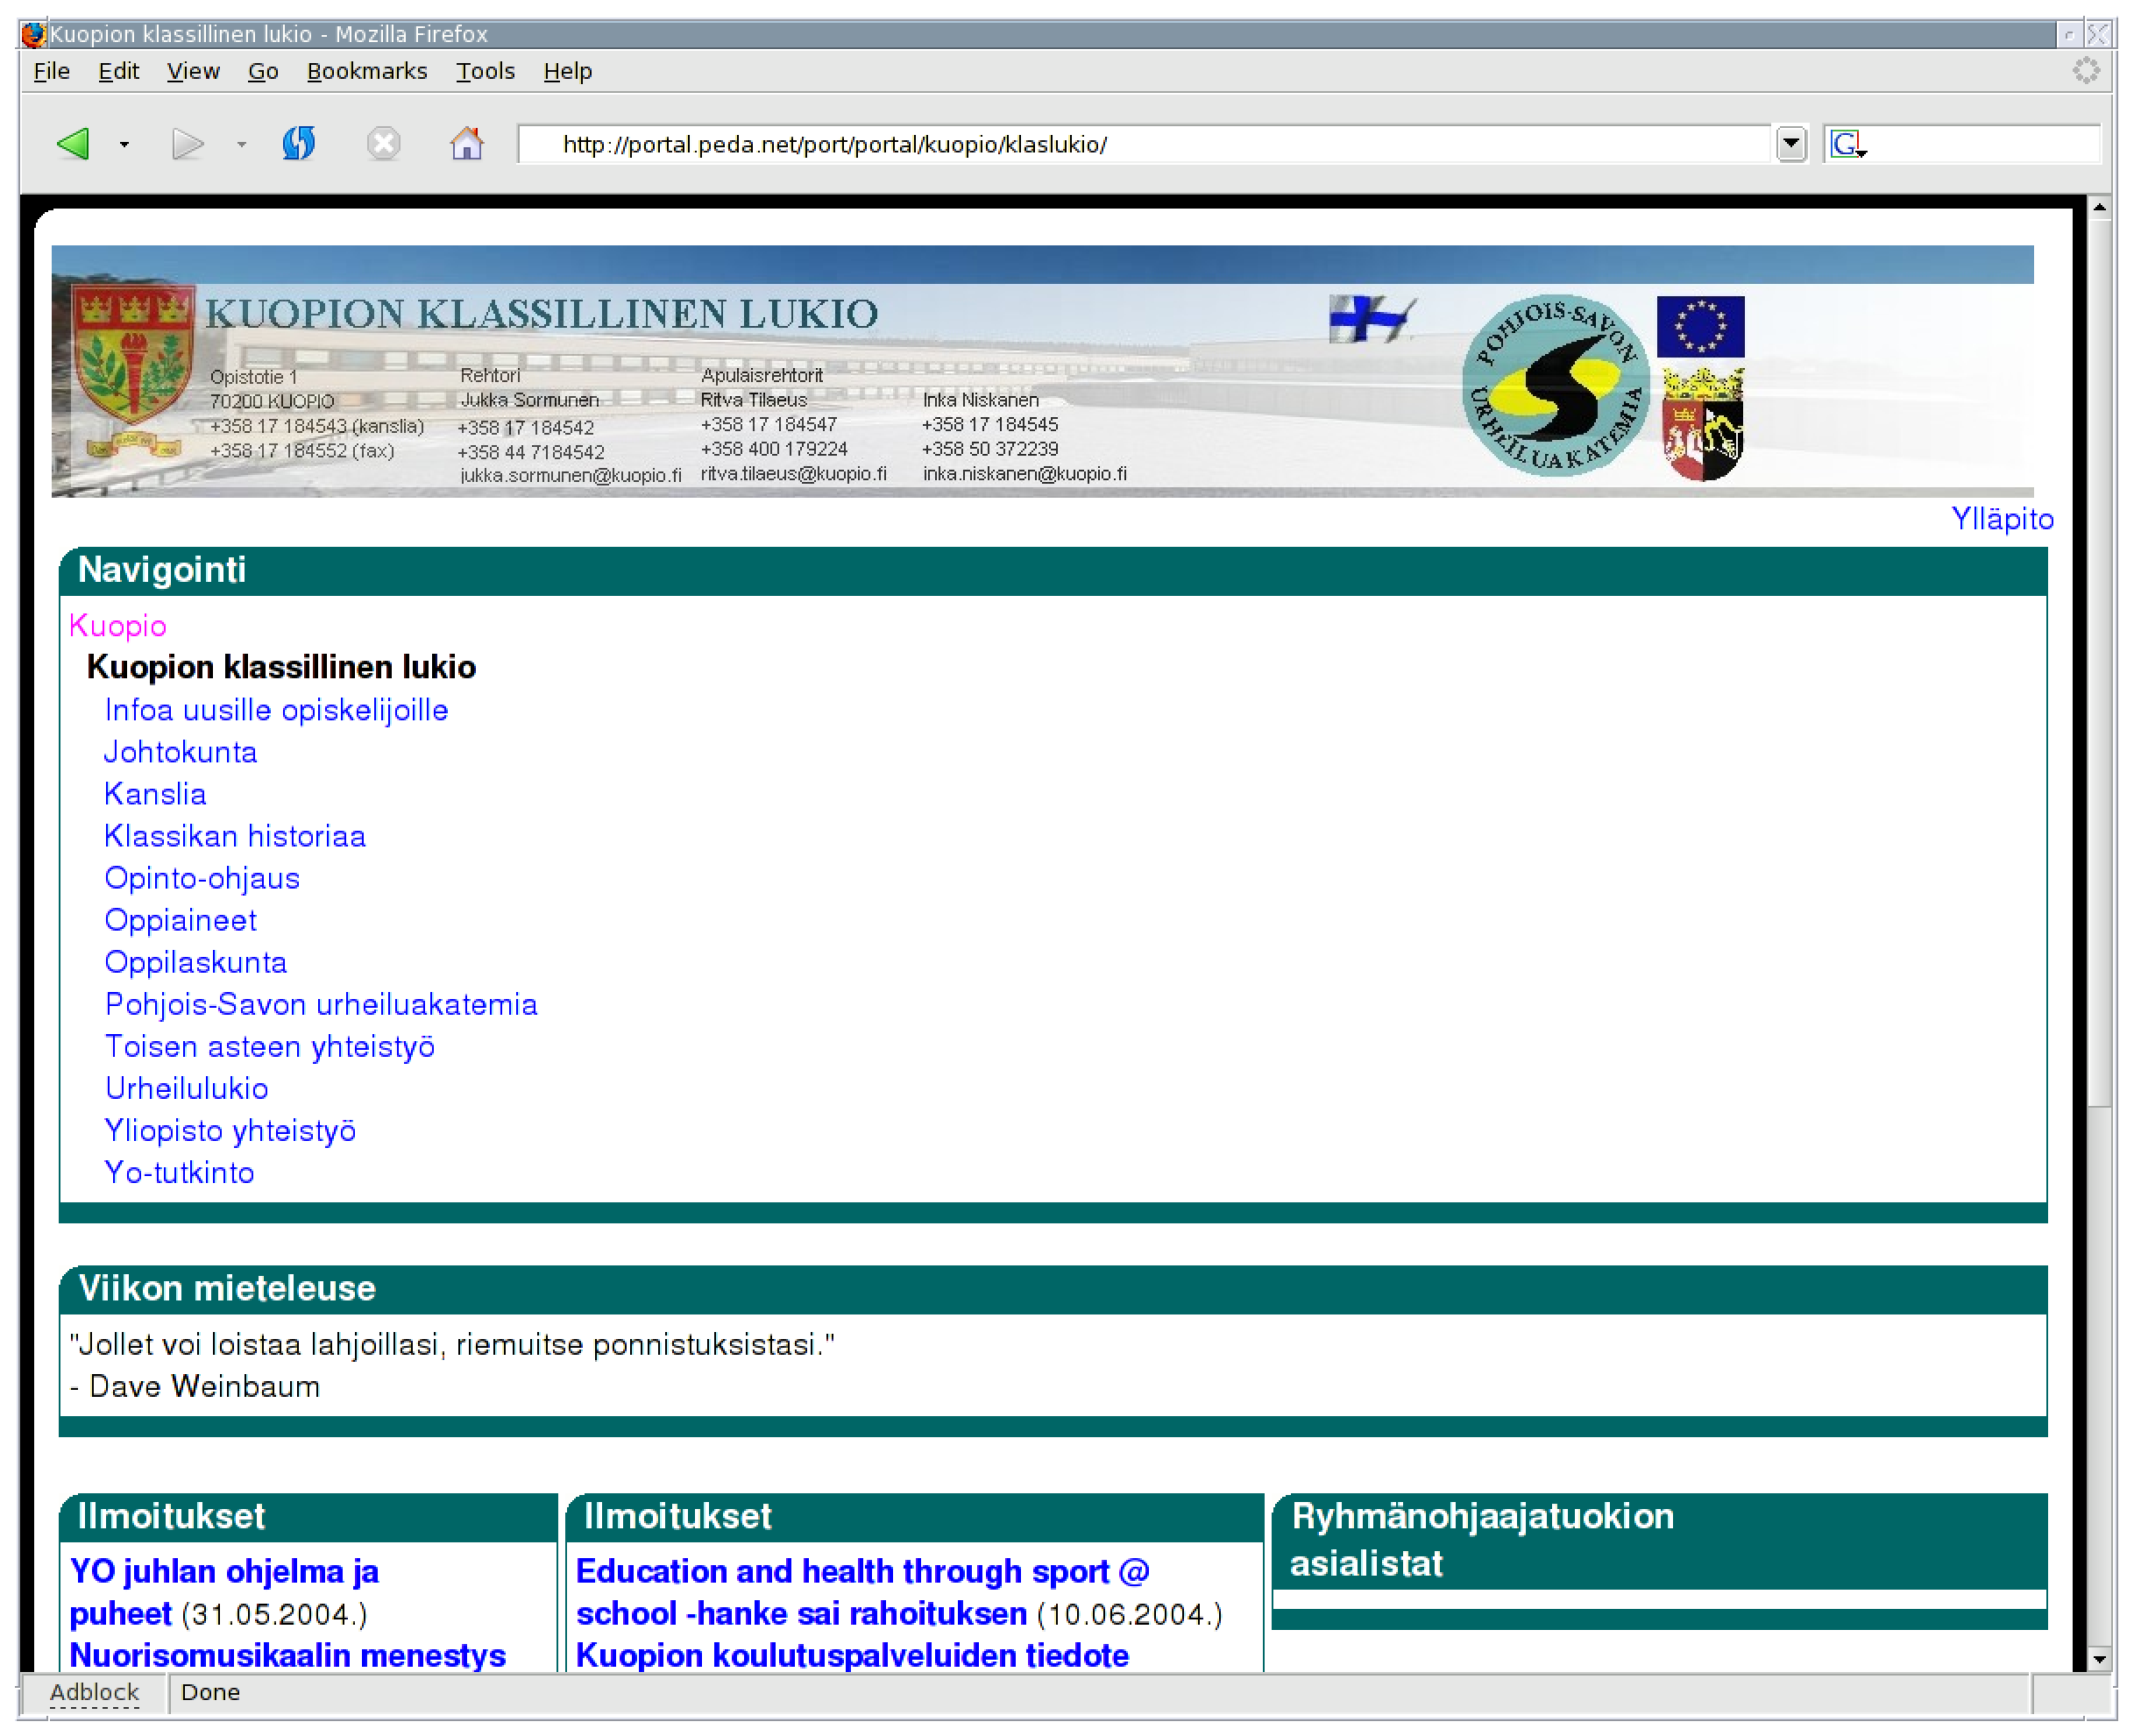
\includegraphics[width=\linewidth]{kuvat/lukio1}
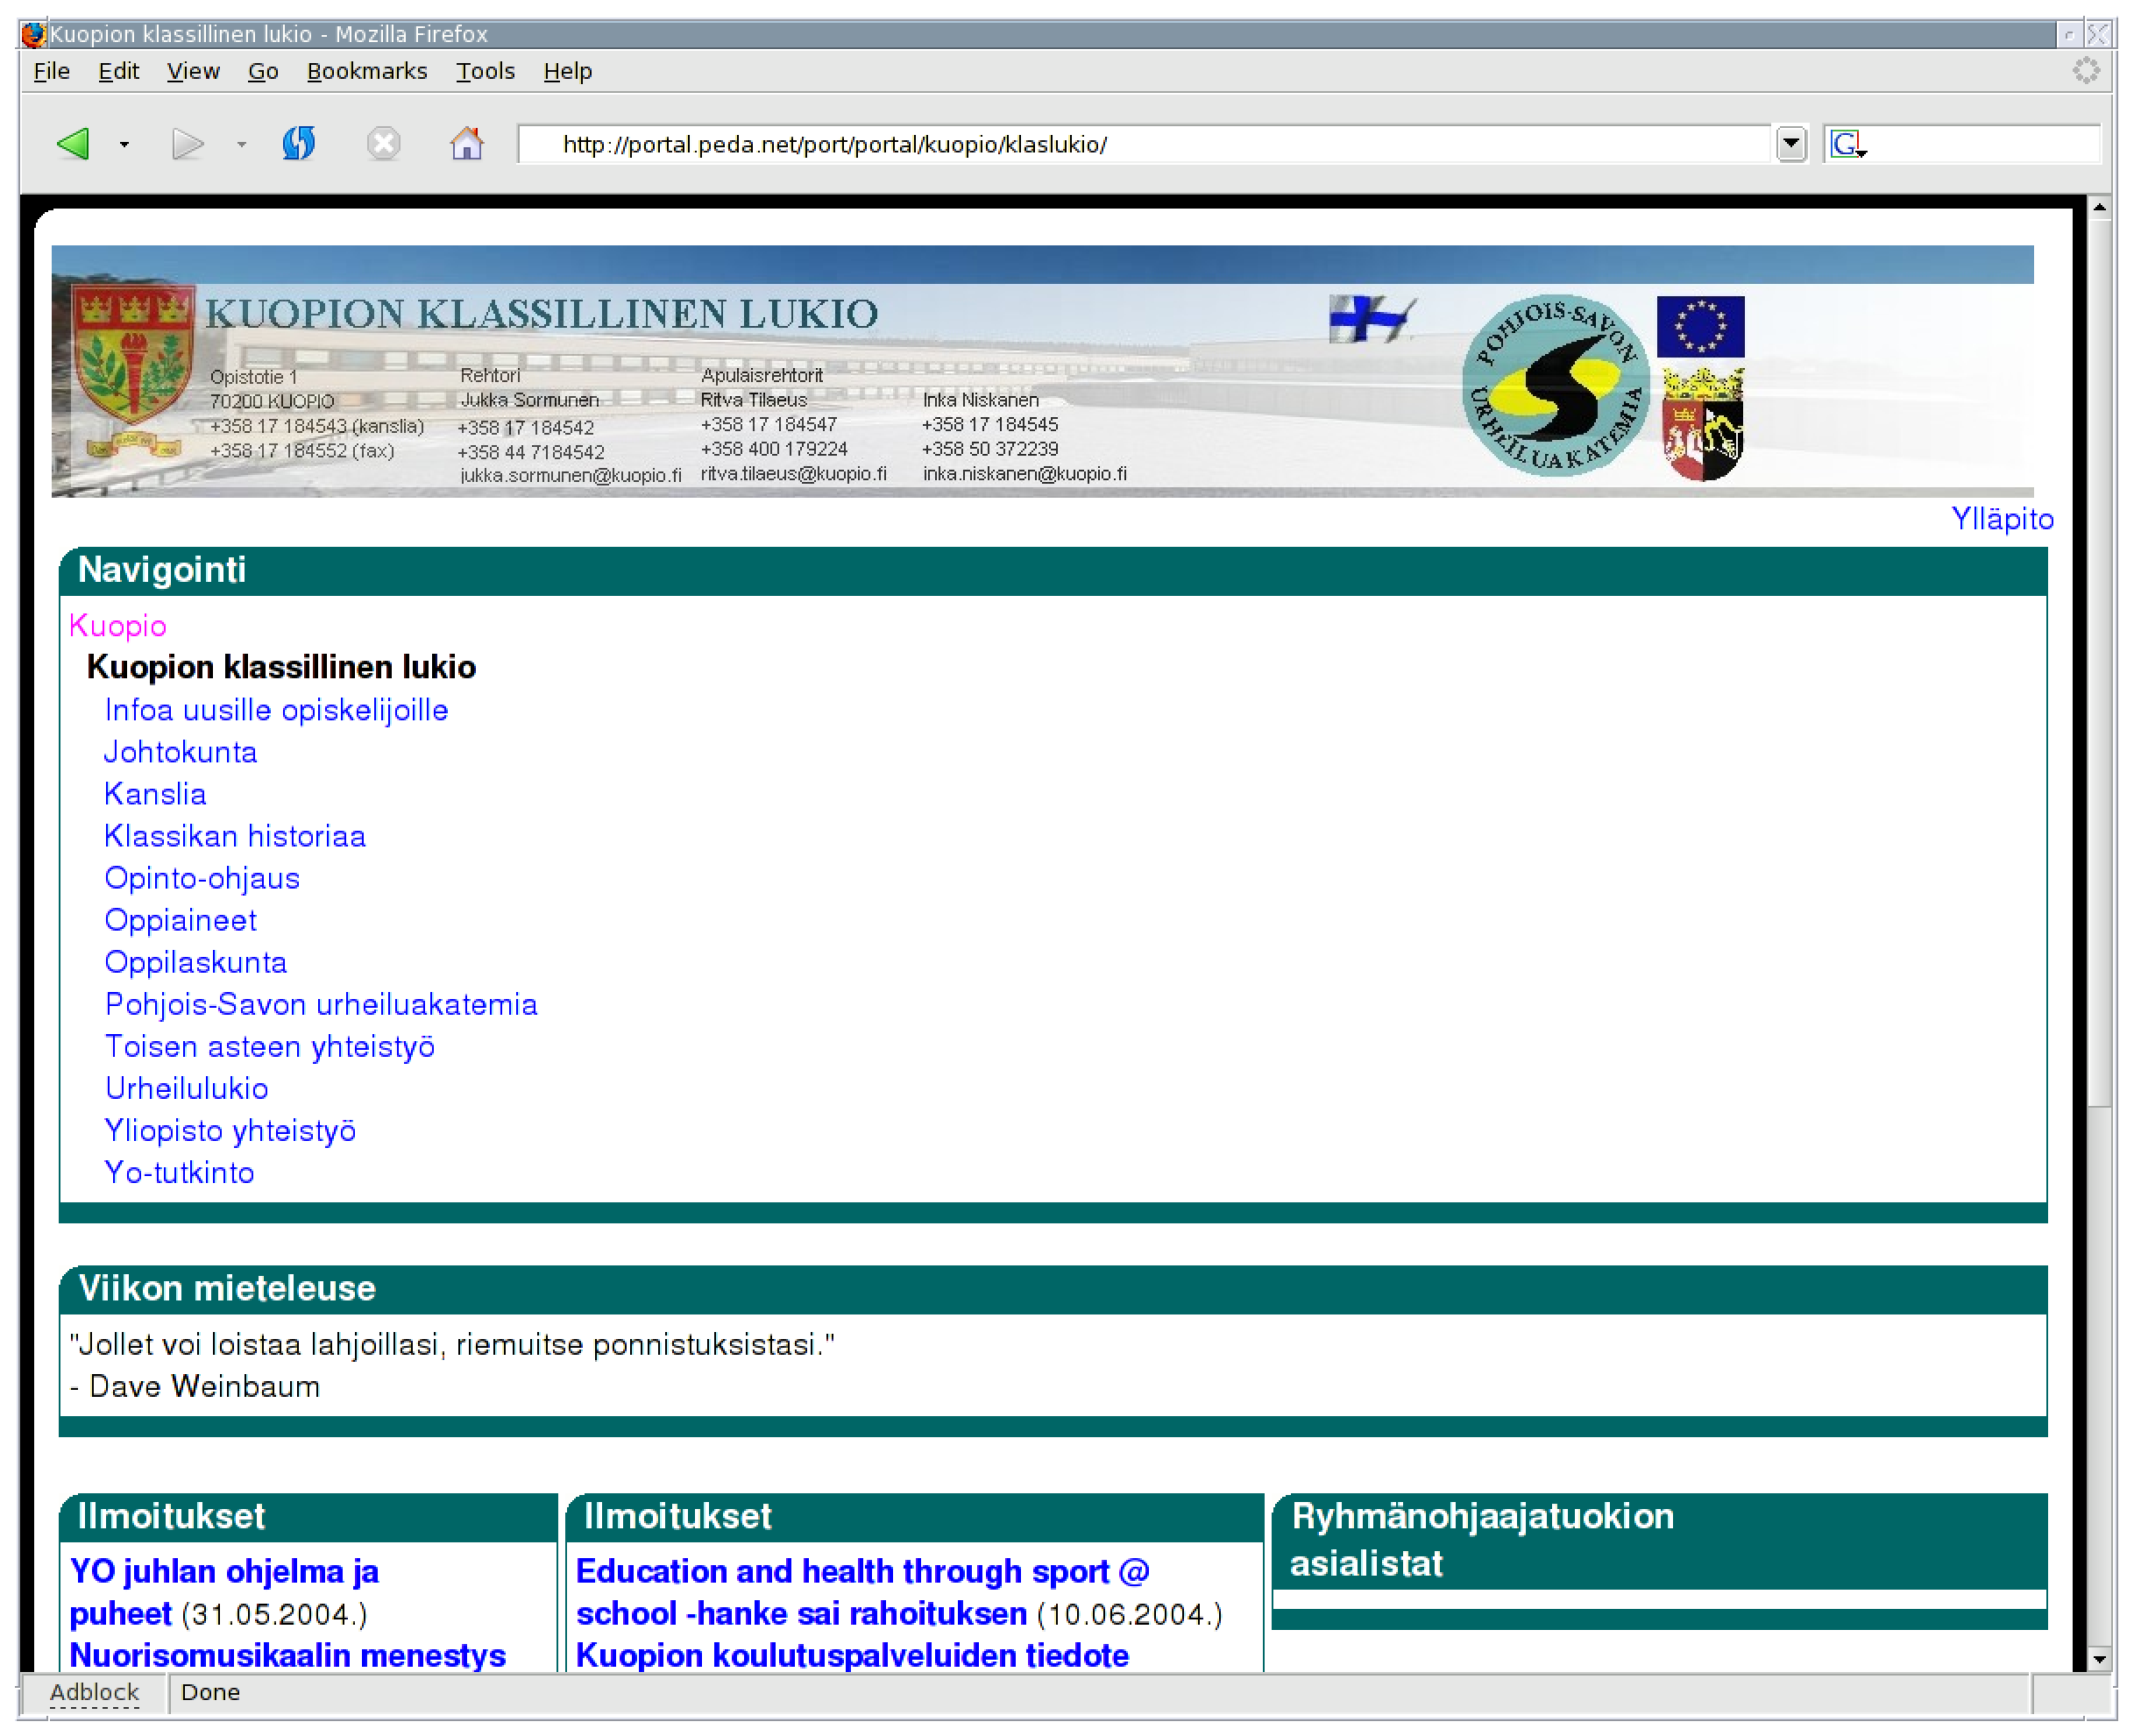
\includegraphics[width=12cm]{kuvat/lukio1}
\caption{Kuopion Klassillisen lukion ver�j�}
\label{fig:veraja1}
\end{kuva}

\begin{kuva}
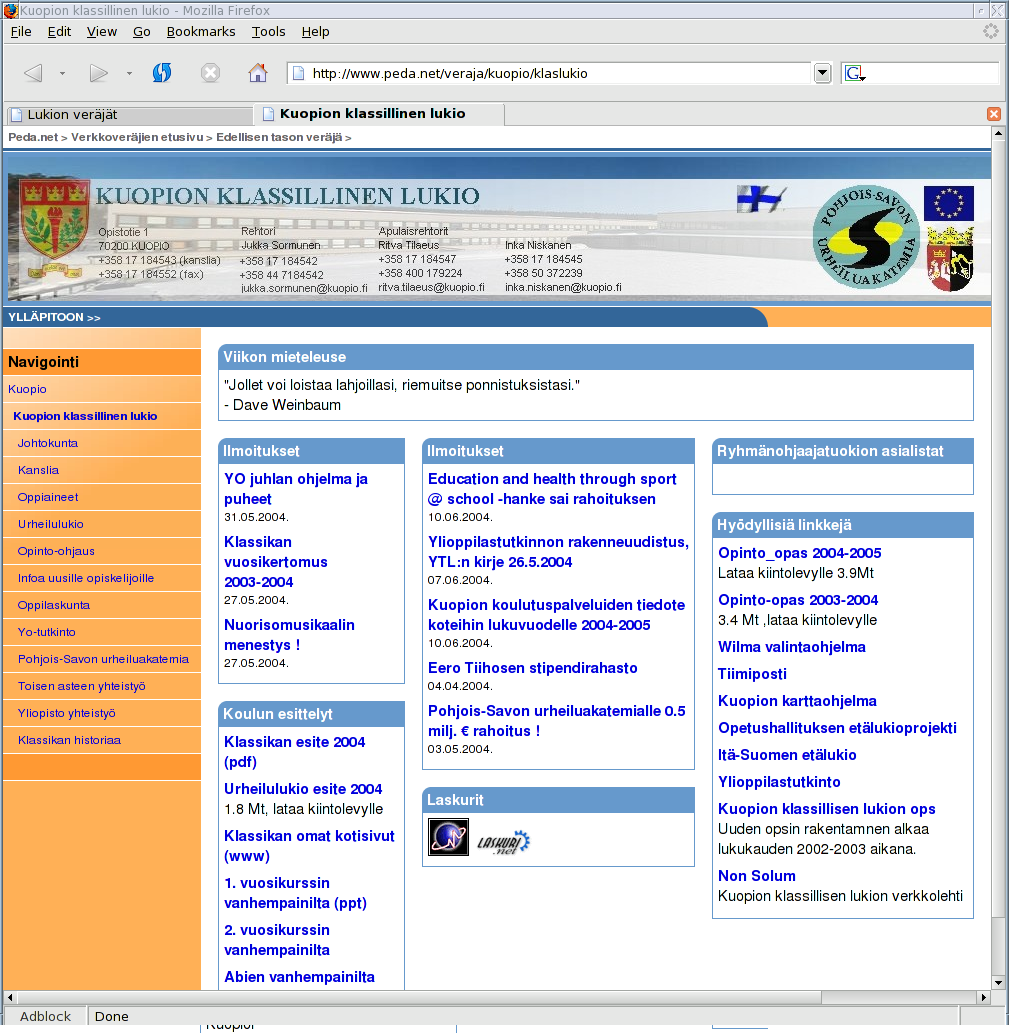
\includegraphics[width=10cm]{kuvat/lukio2}
\caption{Kuopion Klassillisen lukion ver�j� (uusi k�ytt�liittym�)}
\label{fig:veraja2}
\end{kuva}

Portaalissa eli \emph{Verkkover�j�ss�} alkuper�isen� ideana oli tarjota
koulun opettajalle mahdollisuus yll�pit�� opiskelua tukevaa www"-sivua
tai "=sivustoa ilman ohjelmointitaitoa tai www"-sivujen
yll�pito"-ohjelmistoja. Yleisemp�n� k�ytt�tarkoituksena oli tukea my�s
yleisemmin www"-sivujen tuotantoa -- esimerkiksi koulun kotisivujen
muodossa. Monilla kouluilla ei ollut tuohon aikaan, vuonna 2001, omia
kotisivuja. Useinmiten koulun selaimessa n�kyikin oletuksena
ensimm�isen� paikallisen internet"-operaattorin etusivu. T�m�n
katsottiin palvelevan huonosti itse opetusteht�v��. Verkkover�j�n
yhteydess� www"-sivulla tarkoitetaan pelk�n tekstin ja kuvien
julkaisemisen lis�ksi esimerkiksi verkkokeskusteluja tai vastaavaa
toimintaa. Sivu kootaan ns. moduuleista, joita ladotaan
k�ytt�liittym��n tarjolla oleviin layout-malleihin. Ideana on, ett�
yksi moduuli tarjoaa yhden toiminnon: esimerkiksi kuva"-moduulilla voi
sivulle liitt�� kuvan ja kuvatekstin. Kuvassa \ref{fig:veraja1} on
esimerkkin� Kuopion Klassillisen lukion ver�j� alkuper�isen Ver�j�n
k�ytt�liittym�n kautta tarkasteltuna.

Verkkover�j� oli viimeinen Peda.netiss� Perl"-ohjelmointikielell�
toteutettu ja julkaistu sovellus. Verkkover�j� toimi MySQL"-tietokannan
p��ll� ja nykyisin k�yt�ss� oleva, Juha Lahden PHP"-ohjelmointikielell�
vuonna 2004 kirjoittama versio, k�ytt�� edelleen p��piirteilt��n samaa
tietokantaa. Kev��ll� 2004 verkkover�ji� oli k�yt�ss� noin 13000.
Kuvassa \ref{fig:veraja2} on Kuopion Klassillisen lukion ver�j� uuden
k�ytt�liittym�n kautta katseltuna.

\subsection{Portal2"-prototyyppi}

Portaalista eli verkkover�j�st� ryhdyttiin kehitt�m��n toista versiota
vuonna 2002. Kehitys eteni t�ysin toimivan prototyypin toteutukseen
asti. Uusi versio tarjosi mahdollisuuden vaikuttaa portaalin ulkon�k��n
huomattavasti enemm�n ja merkitt�v�n� toiminnallisena uutuutena
moduuleita voitiin tarjota julkisesti tarjolle muiden opettajien
ver�jiin. T�ll�in esimerkiksi yksitt�isen opettajan tuottamaa
matematiikan aineistoa voitaisiin k�ytt�� toisen koulun matematiikan
kurssilla, integroituna muuhun sen kurssin k�ytt�m��n materiaaliin.

%\begin{kuva}
%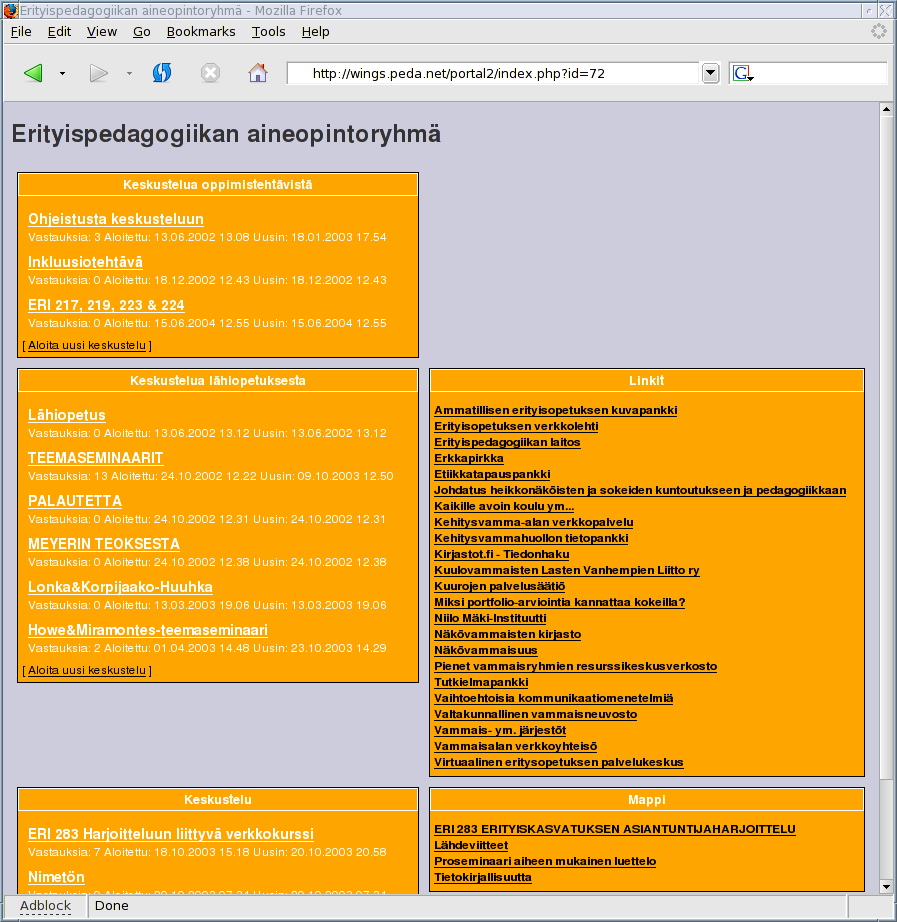
\includegraphics[width=10cm]{kuvat/portal2}
%\caption{Kuva Portal2"-prototyypist�}
%\label{fig:portal2}
%\end{kuva}

\begin{kuva}
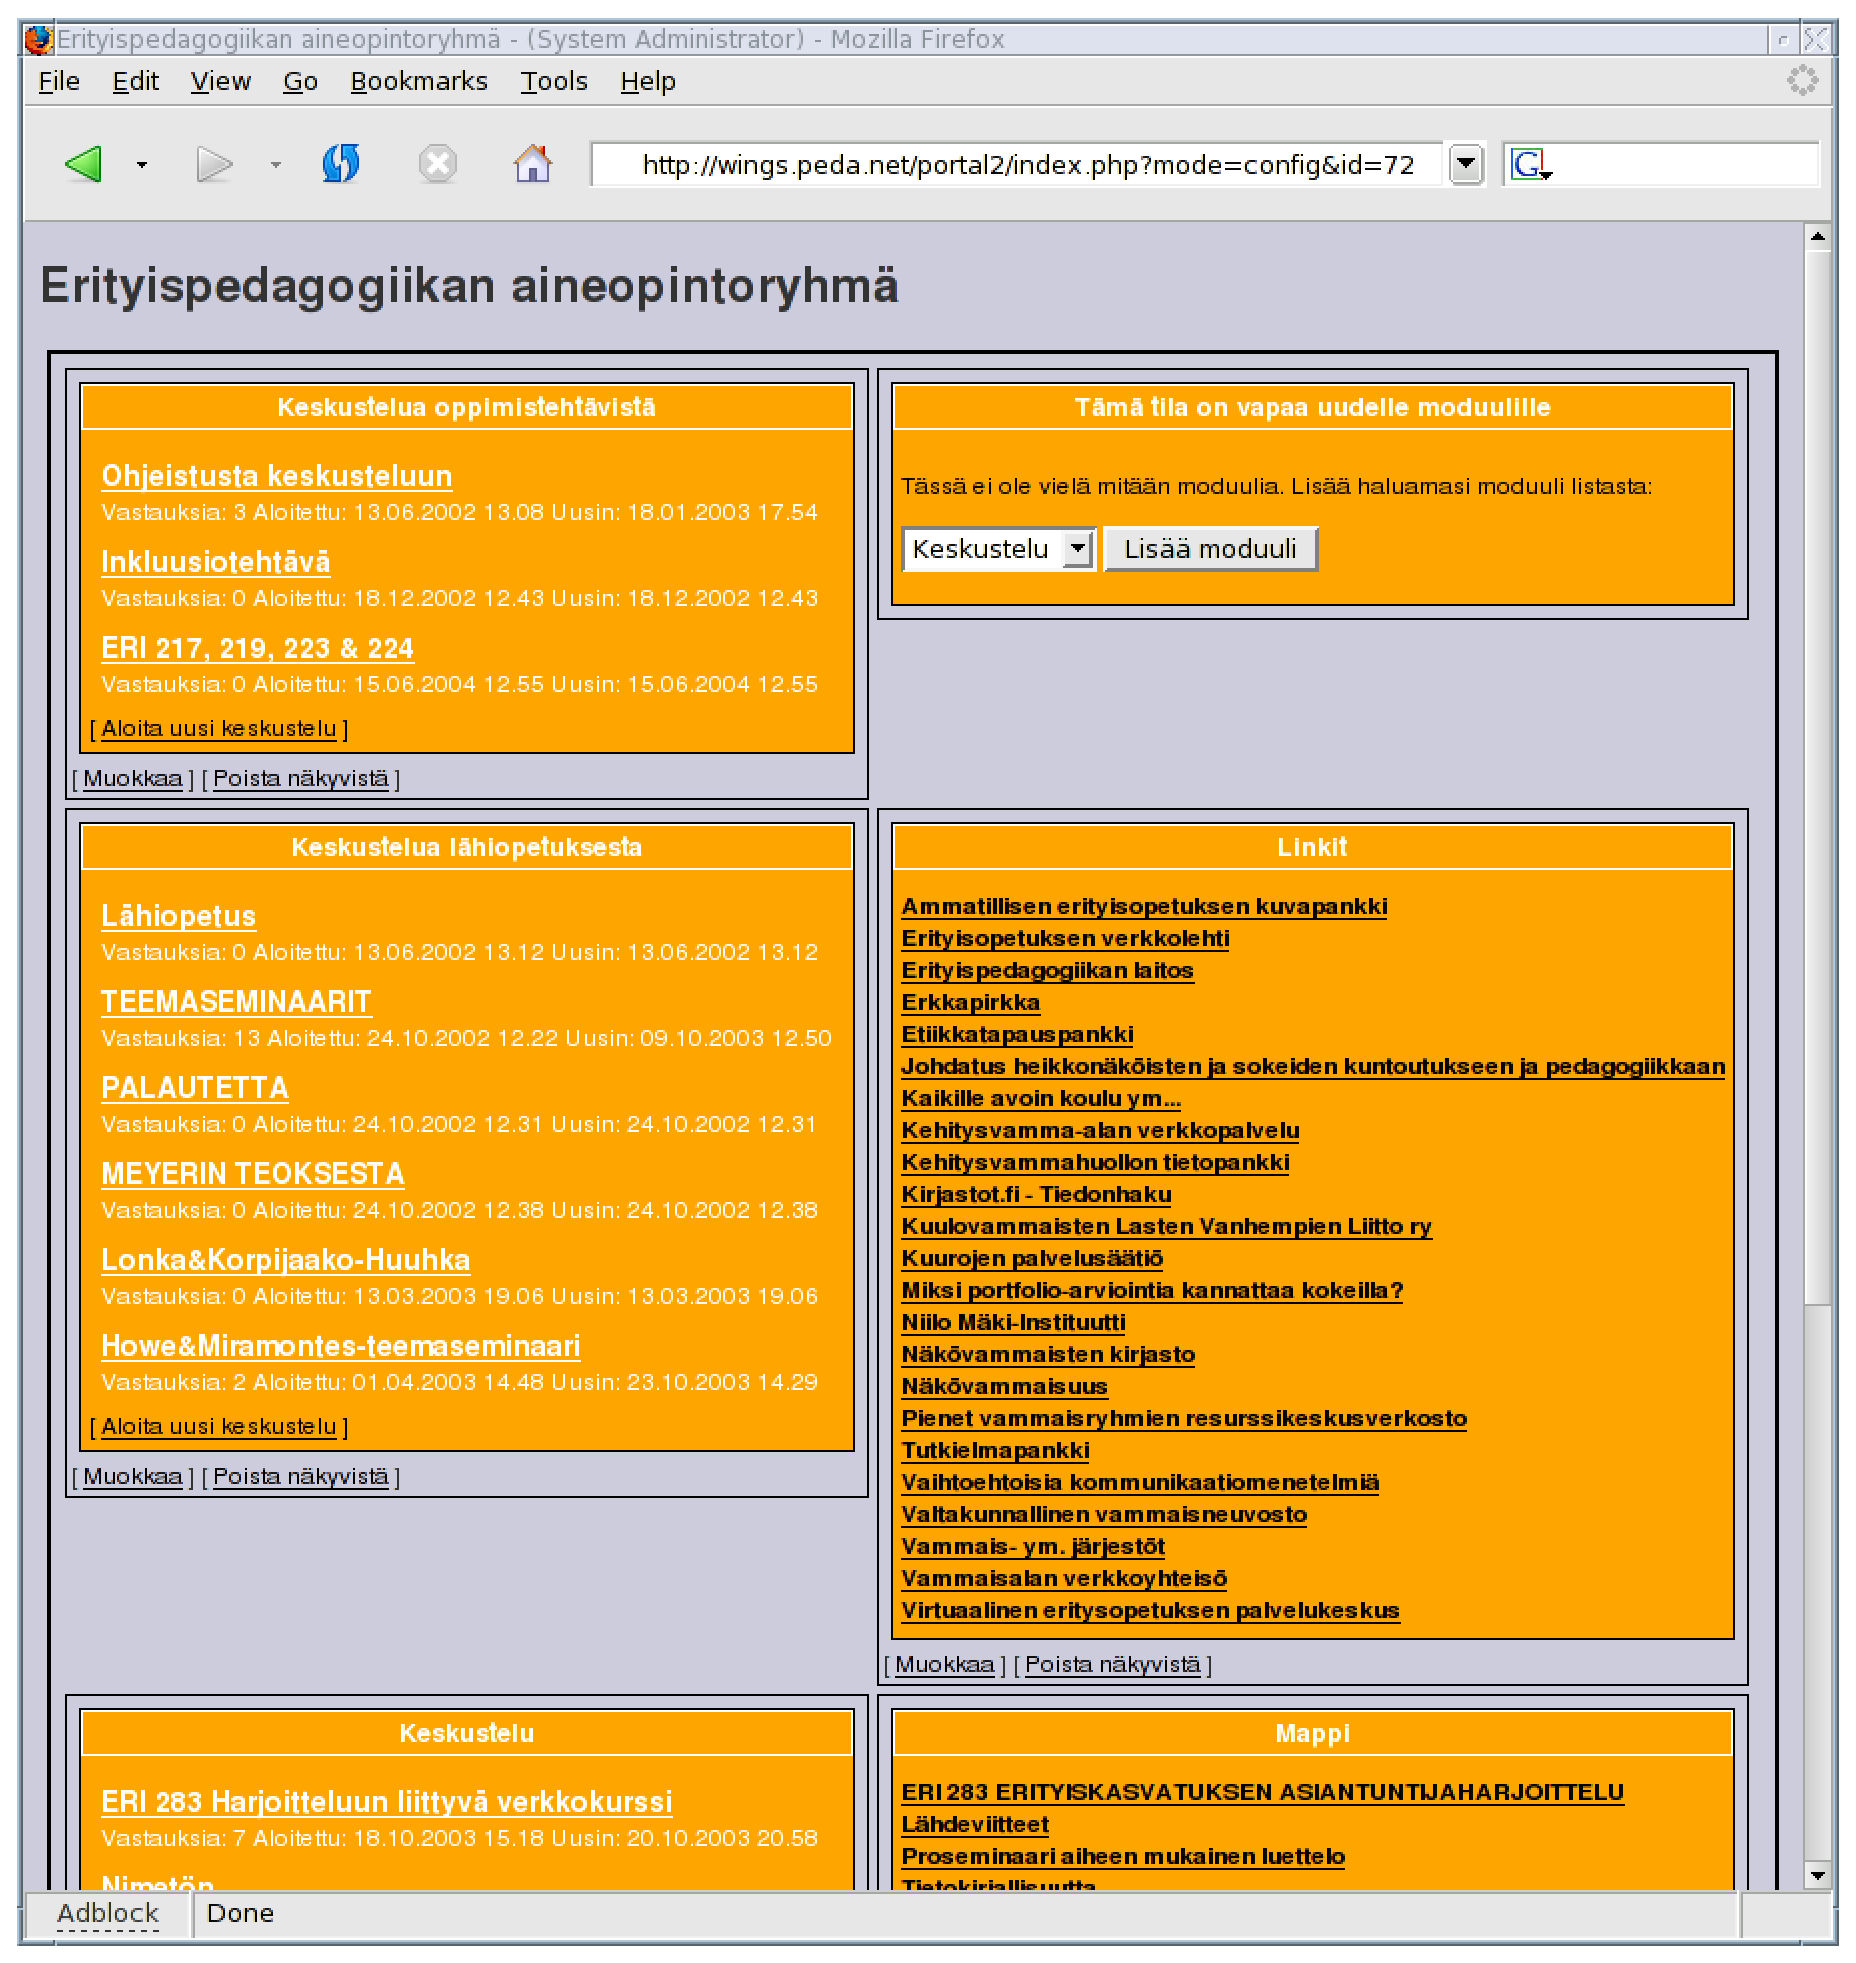
\includegraphics[width=10cm]{kuvat/portal22}
\caption{Kuva Portal2"-prototyypin yll�piton�kym�st�}
\label{fig:portal22}
\end{kuva}

Ohjelma tehtiin uuden tietokantarakenteen p��lle, mutta my�hemmin
p��dyttiin tulokseen, ett� uuden version tarjoamat uudet toiminnot
eiv�t tuoneet riitt�v�sti etuja, jotta vanhan version k�ytt�jien olisi
kannattanut siirty� k�ytt�m��n uutta versiota. My�sk��n kahden
rinnakkaisen, miltei samaan k�ytt��n tarkoitetun sovelluksen
yll�pit�miseen ei haluttu ryhty�. My�s Portal2 tehtiin viel�
Perl"-ohjelmointikielell� MySQL"-tietokannan p��lle. Puutteistaan
huolimatta Portal2 on ollut pienimuotoisessa k�yt�ss� siin� kunnossa
kuin se on ja sit� k�ytt�en on j�rjestetty Avoimen Yliopiston kursseja
viel� talvella 2004.

Juha Lahti kirjoitti Ver�j�st� kev��ll� 2004 julkaistun kolmannen
version; se sis�lsi osan samoista toiminnoista kuin Portal2, tosin
moduulien jakamista ei ole ainakaan viel� toteutettu. Kolmas versio
p��tettiin kehitt�� yhteensopivaksi ensimm�isen kanssa, jolloin
kaikkien vanhojen portaalien sis�lt� olisi v�litt�m�sti k�ytett�viss�
my�s uuden k�ytt�liittym�n kautta. Siirtym�vaiheessa (k�yt�nn�ss�
vuoden 2004 alusta saman vuoden syksyyn) portaalien k�ytt� ja yll�pito
onnistuu molempien k�ytt�liittymien kautta. Vanha k�ytt�liittym�
poistetaan k�yt�st� mahdollisimman nopeasti, jotta tulevaisuudessa
uusia ominaisuuksia lis�tt�ess� tarvitsee huomioida ainoastaan uusin
k�ytt�liittym�.

\subsection{YALE2"-prototyyppi}

YALE2 eli Yet Another Learning Environment 2 on kokonaan
PHP"-ohjelmointikielell� vuonna 2003 uudelleenkirjoitettu versio Juha
Lahden tekem�st� YALE"-prototyypist�. YALE2 on selaink�ytt�inen
oppimisymp�rist� yksitt�isen koulun k�ytt��n. YALE2 tarjosi
suljettujen, oppilaiden k�ytt��n luotujen kurssien luomisen ja
yll�pidon lis�ksi julkaisumahdollisuuden kirjasto"-nimisen
ominaisuuden muodossa.

YALE2 on t�t� kirjoittaessa (kev��ll� 2004) edelleen pienimuotoisessa
testik�yt�ss�, mutta sit� ei tulla virallisesti ottamaan k�ytt��n
miss��n vaiheessa. Sovellus poistetaan k�yt�st� todenn�k�isesti t�m�n
vuoden loppuun menness�. YALE2 oli loogisesti Oppimapin esiaste, jossa
ei ollut versionhallintaa ja oikeuksien hallinta oli huomattavasti
rajoittuneempaa. Lis�ksi k�ytt�liittym�n rakenteessa oli joitakin
k�ytett�vyysongelmia. Uuden version kehitt�miseen p��dyttiin, koska
versionhallinnan ja kehittyneemm�n oikeuksien hallinnan liitt�minen
t�h�n versioon arvioitiin ty�l��mm�ksi kuin kokonaan uuden j�rjestelm�n
kehitt�minen.

%\begin{kuva}
%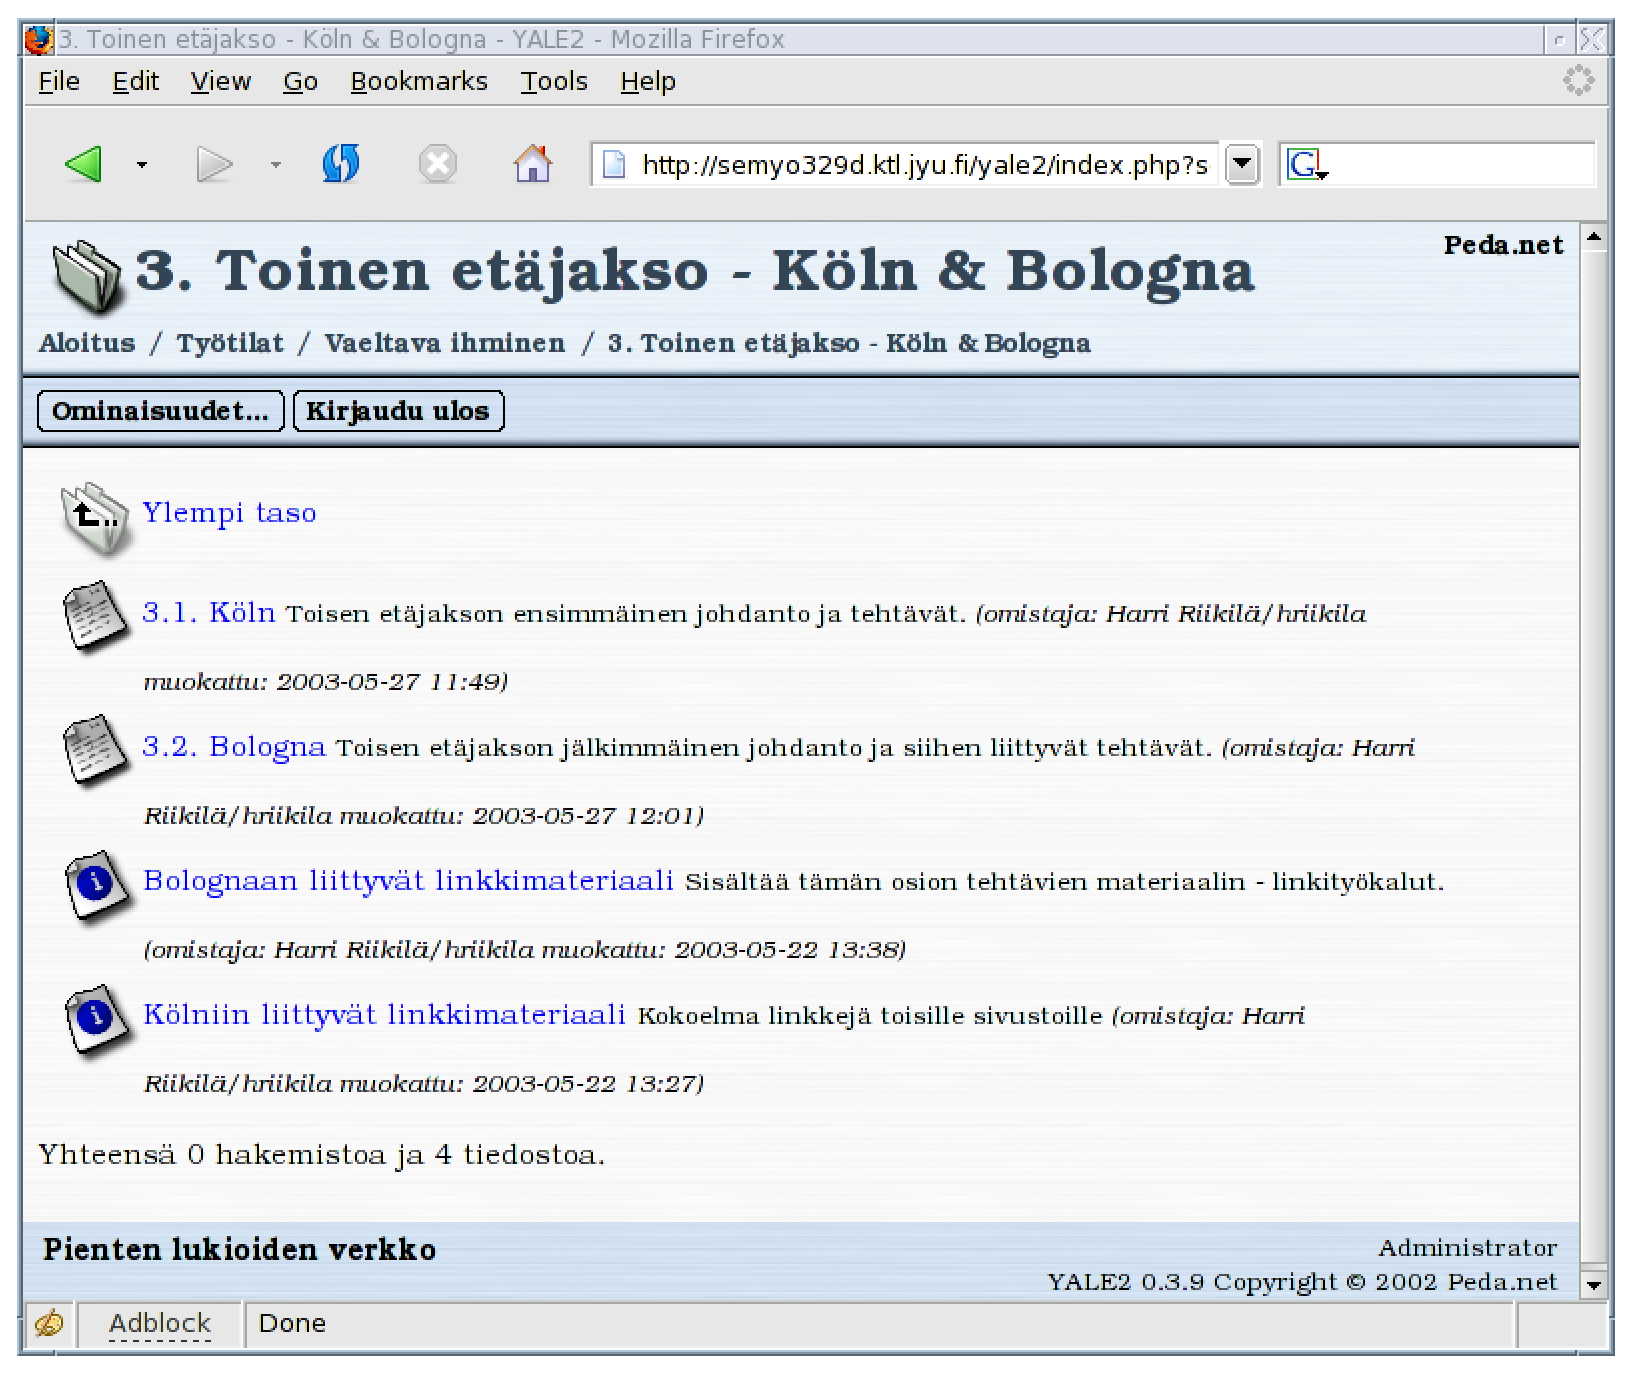
\includegraphics[width=10cm]{kuvat/yale21}
%\caption{YALE2: yksitt�isen kurssin n�kym�}
%\label{fig:yale21}
%\end{kuva}

\begin{kuva}
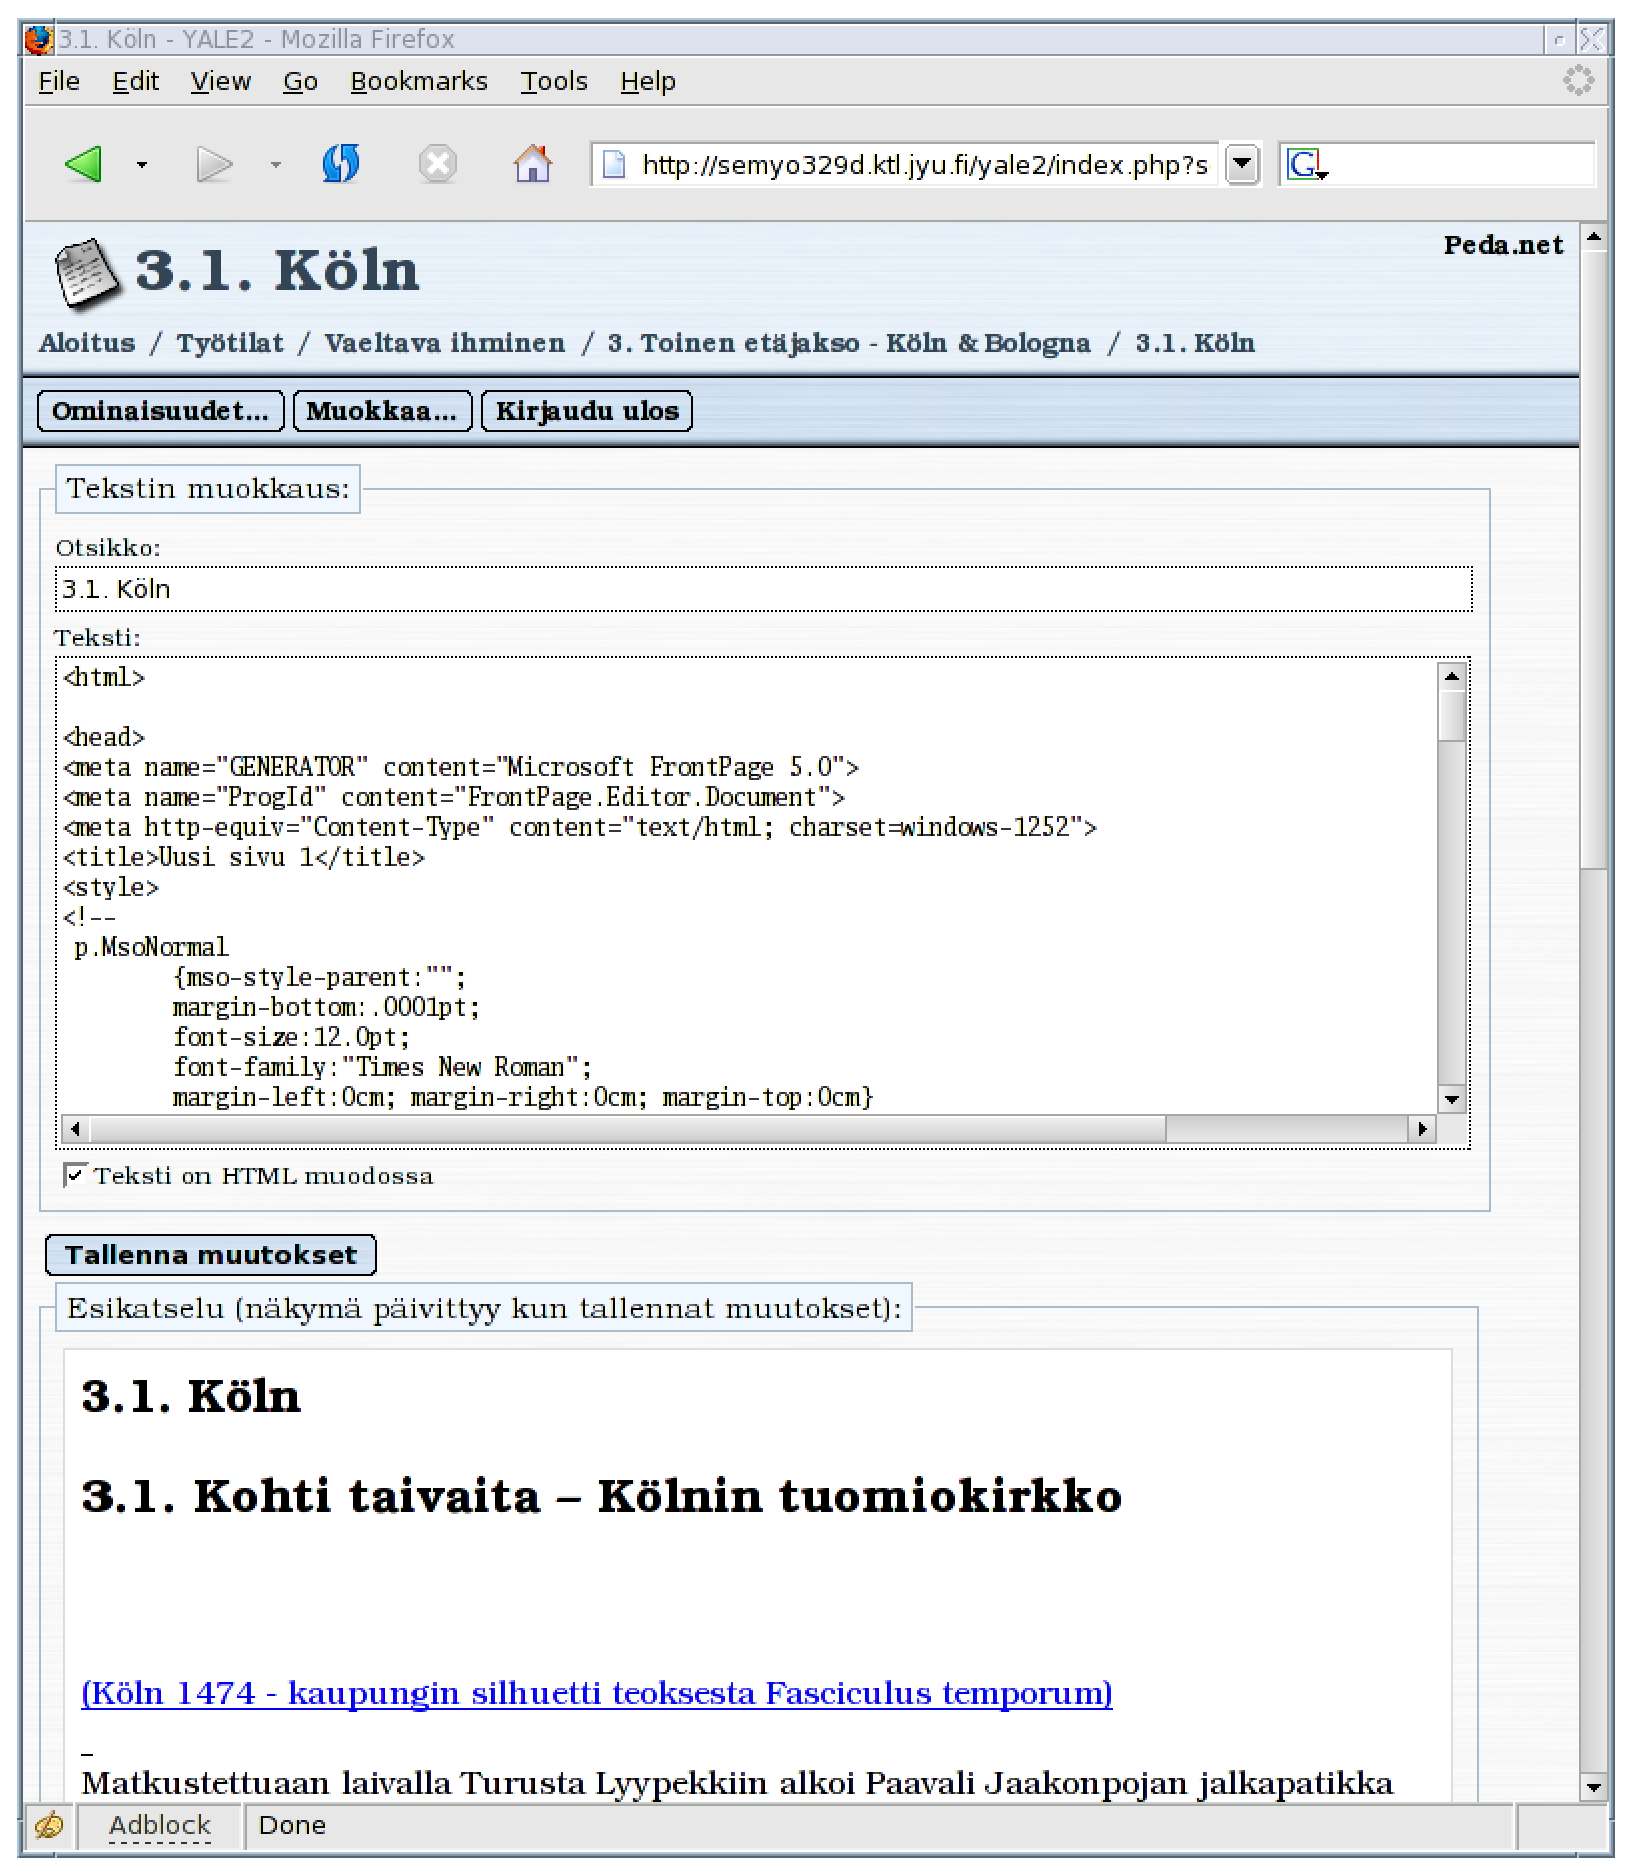
\includegraphics[width=10cm]{kuvat/yale22}
\caption{YALE2: esimerkki kurssin materiaalin muokkaamisesta}
\label{fig:yale22}
\end{kuva}

\subsection{Oppimappi}
\label{pedanet-oppimappi}

Peda.net Oppimappi on kirjoittajan nykyinen kehitysprojekti, joka
tarjoaa yksitt�isen koulun kaikille kursseille riitt�v�n
oppimisymp�rist�n.T�m� sovellus ei tue kurssien j�rjest�mist� usean eri
oppilaitoksen kesken, vaan se on suunniteltu yksitt�isen koulun
tarpeita varten. Rajaukseen p��dyttiin, koska ohjelman toteuttamisen
ty�m��r�n arvioitiin kasvavan liian suureksi nykyisiin resursseihin
verrattuna. Sovellusta on kehitetty kes�st� 2003 alkaen ja se
julkaistiin syksyll� 2004. Kuten selaink�ytt�isten sovellusten
tapauksessa yleens�, julkaisu ei tarkoita sovelluksen kehityksen
lopettamista t�ss�k��n tapauksessa. Uusia ominaisuuksia tullaan
lis��m��n julkaisun j�lkeen k�ytt�jien toiveiden mukaan. Samoin
k�ytt�liittym� k��nnet��n eri kielille; tuetut kielet sis�lt�v�t
ainakin suomen, ruotsin, englannin, saksan ja saamen.

\begin{kuva}
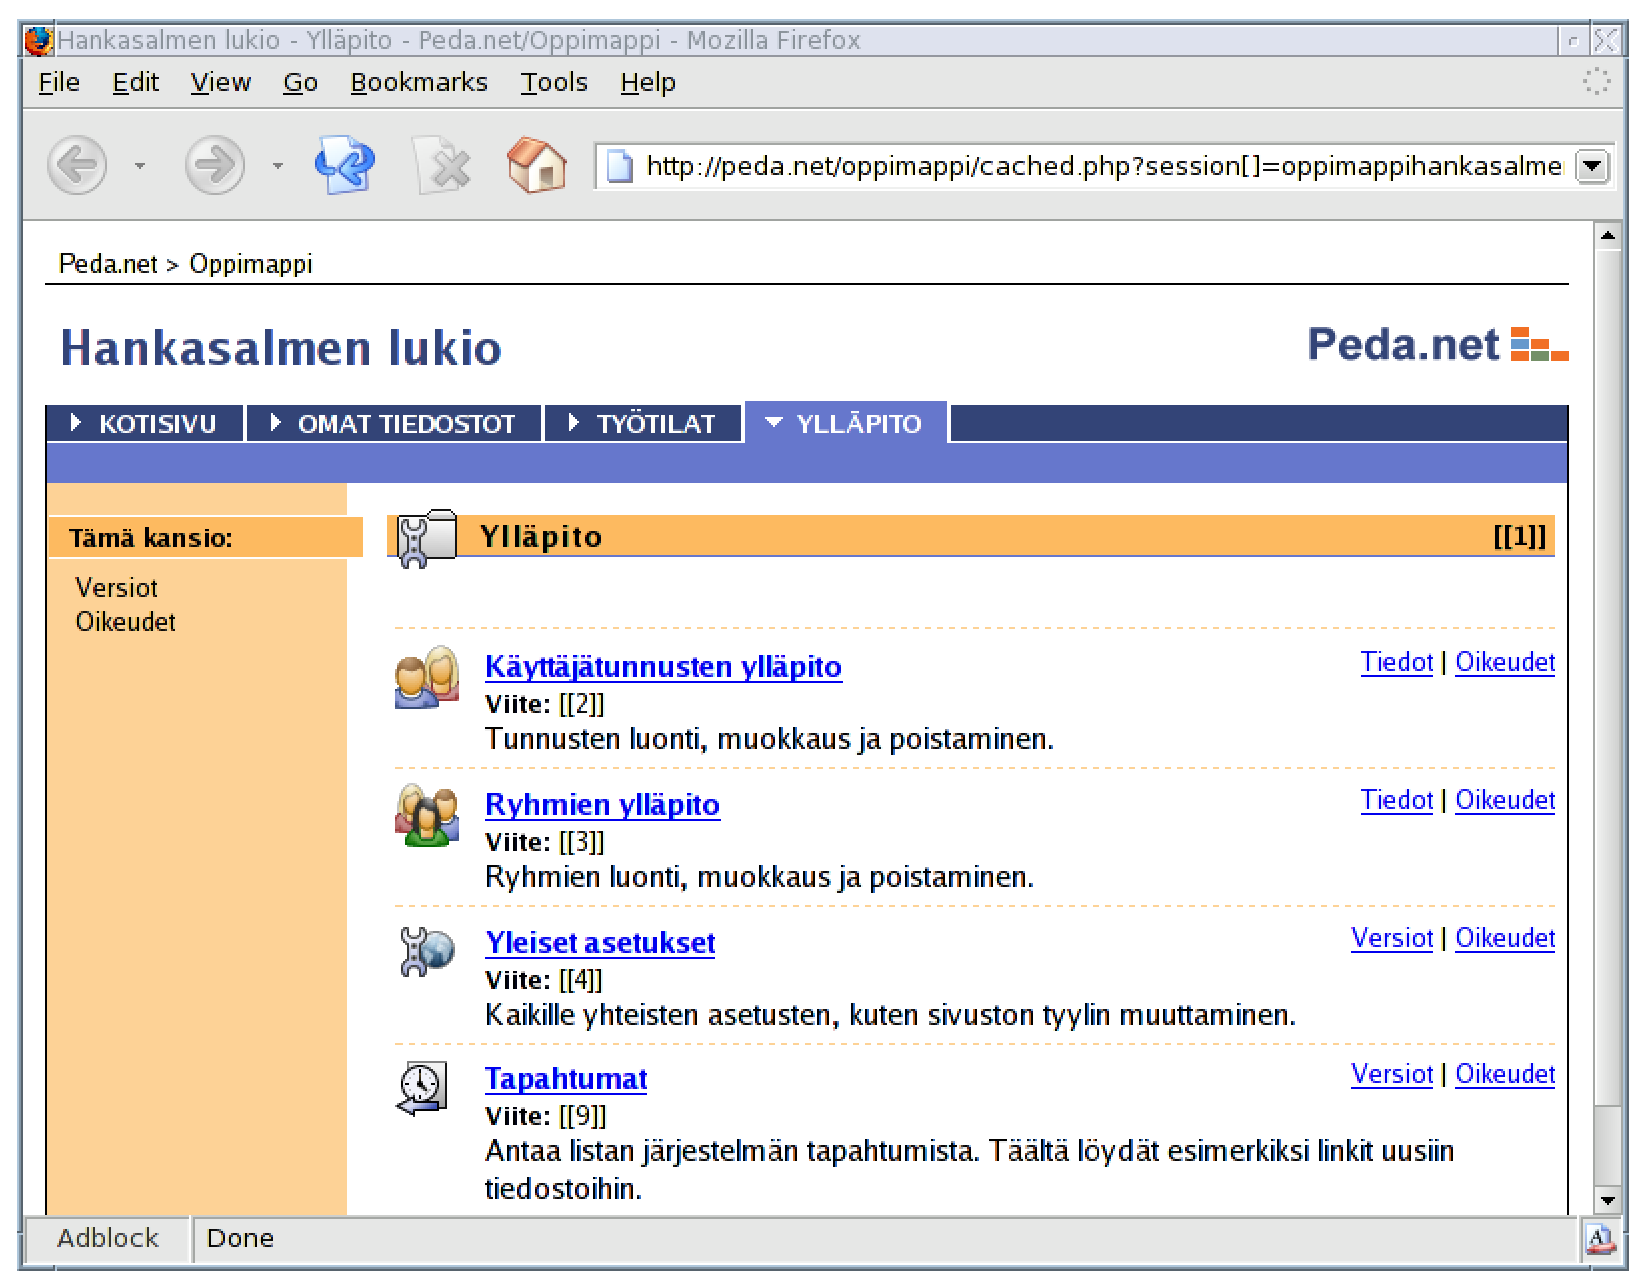
\includegraphics[width=10cm]{kuvat/oppimappi}
\caption{Esimerkki Oppimapin k�ytt�liittym�st�}
\label{fig:oppimappi}
\end{kuva}

Yll�pit�j�n kannalta merkitt�vi� ominaisuuksia ovat k�ytt�jien hallinta
monitasoisten ryhmien kautta, kurssien ja kurssimateriaalien oikeuksien
m��rittely luku- ja kirjoitusoikeuksien avulla ja versionhallinta sek�
kaiken materiaalin vapaa linkitt�minen mihin tahansa j�rjestelm�n
sis�ll�. Loogisella tasolla Oppimapissa yll�pidet��n kaksisuuntaista
hierarkiaa, joka muodostuu erilaisista dokumenttityypeist� tai
moduuleista. Eri dokumenttityyppej� ovat muun muassa kansiot,
tiedostot, keskustelut ja ty�tilat. Jokainen moduuli voi sis�lt�� muita
moduuleita ja jokainen moduuli voi n�ky� monen eri moduulin sis�ll�.
Tietokanta mahdollistaa jopa moduulin n�kymisen itsens� sis�ll�. Osaa
toiminnoista on rajoitettu k�ytt�j�n toimien helpottamiseksi.
Esimerkiksi k�ytt�liittym� ei tarjoa mahdollisuutta luoda ty�tiloja
keskustelun sis�lle (tosin olemassaolevaan ty�tilaan voi viitava keskustelussa, jolloin j�rjestelm� tarjoaa polun kulkea kyseiseen ty�tilaan keskustelun kautta).

\subsection{Muu Peda.netiss� tapahtunut sovelluskehitys}

Lis�kseni Peda.net"-hankkeessa on tehnyt
ohjelmistokehityst� Juha Lahti, joka on kehitt�nyt mm. seuraavat
sovellukset:

\begin{itemize}
\item Verkkolehti (testik�yt�ss� olleita prototyyppej�, 1997-1999)
\item Verkkolehti (Juhan opinn�ytety�, 2001?)
\item OPSpro (nykyisin k�yt�ss� oleva kolmannen sukupolven versio, 2002)
\item Verkkover�j� (ty�nimi: Portal3, 2004)
\item Verkkolehti (ty�nimi: Verkkolehti2, 2004)
\end{itemize}

N�ist� verkkolehden nykyisell� versiolla toimivia lehti� oli noin 2200
kappaletta tammikuussa 2004. Eri ver�ji� oli noin 13000 ja
OPSpro-sovelluksella toteutettuja opetussuunnitelmia noin 600.

Peda.net on t�ll� hetkell� Suomen johtava oppimisymp�rist�jen
toimittaja k�ytt�j�m��r�ss� mitattuna.

\section{Oppimapin k�ytett�vyyden arviointia}

\begin{kuva}
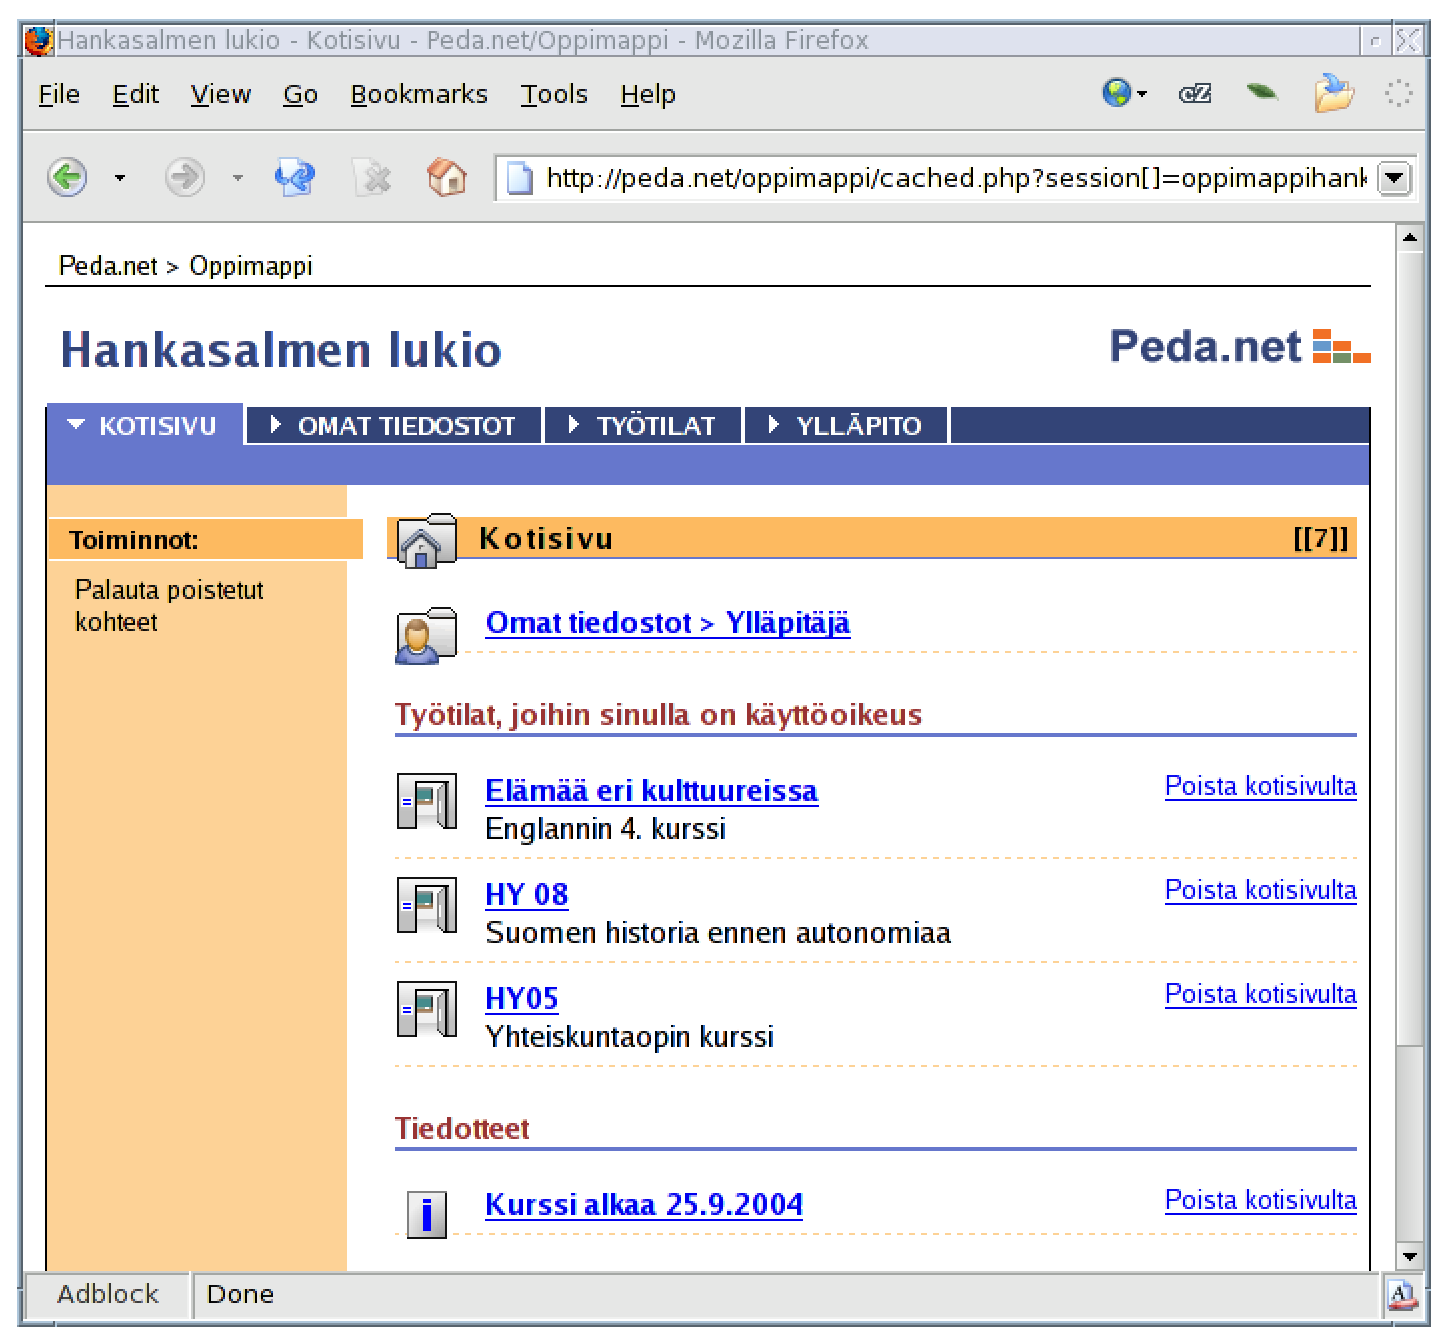
\includegraphics[width=10cm]{kuvat/oppimappi-kotisivu}
\caption{Oppimappi: ty�p�yt�-n�kym�}
\label{fig:oppimappi-kotisivu}
\end{kuva}

Oppimapin k�ytt�liittym�n p��osat muodostuvat navigointipalkista,
toimintovalikosta ja sis�lt�alueesta. Kuvassa
\ref{fig:oppimappi-kotisivu} on esitetty Oppimapin kotisivu-n�kym�
yll�pit�j�n oikeuksilla. T�m� on Oppimapin aloitussivu
sis��nkirjautumisen j�lkeen. Yl�reunassa n�kyy Oppimapin otsikko (t�ss�
esimerkiss� ``Hankasalmen lukio'') ja linkit eri alueille Oppimapin
sis�ll�: kotisivu, omat tiedostot, ty�tilat ja yll�pito. Vasemman
reunan palkissa on aina sen hetkist� sis�lt�� koskevat toiminnot, t�ss�
tapauksessa  vain ''palauta poistetut kohteet'', joka palauttaisi
sis�lt�listaukseen ne dokumentit, ty�tilat ja kansiot, jotka k�ytt�j�
on aikaisemmin itse poistanut. Itse sis�lt�alue muodostuu t�ll� sivulla
erilaisista objekteista, joilla jokaisella on ikoni, nimi, kuvaus ja
toimintoja. Nimest� n�p�ytt�m�ll� p��see k�ytt�m��n objektia ja
objektin per�ss� olevaa toimintoa k�ytt�m�ll� sen ominaisuuksiin voi
vaikuttaa.

Ensimm�iseksi havaitaan, ett� t�ss�kin ymp�rist�ss� suuri osa ikkunan
pinta-alasta menee muuhun kuin itse sis�lt��n. Navigointi ja ymp�rist�n
otsikko valtaavat suuren osan k�ytett�viss� olevasta alasta. T�m� on
seurausta valitusta tyylitiedostosta. Kuvassa
\ref{fig:oppimappi-kotisivu-nostyle} on esitetty sama n�kym� kun
CSS-tyylisivu on selaimen asetuksista valittu pois p��lt�. T�m� n�kym�
vastaa erityisryhmien k�ytt�liittym��; esimerkiksi sokealle k�ytt�j�lle
tieto esitett�isiin t�m�n n�kym�n mukaisessa j�rjestyksess�. T�ss�
erityisesti nykyist� n�kyv�� koskevat toiminnot esitet��n sis�ll�n
\emph{j�lkeen} -- t�m� on t�rke��, koska yleens� k�ytt�j� on
kiinnostunut itse sis�ll�st�, ei mahdollisista toiminnoista. Samoin kaikki sovelluksen toiminnallisuus on k�ytett�viss� ilman kuvien lataamista tai JavaScript-tukea.

\begin{kuva}
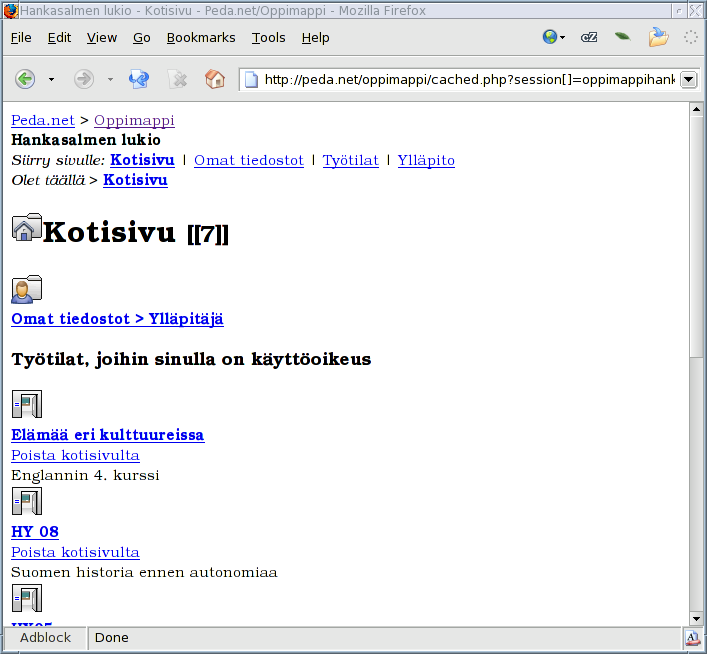
\includegraphics[width=10cm]{kuvat/oppimappi-kotisivu-nostyle}
\caption{Oppimappi: ty�p�yt�-n�kym� ilman CSS-tiedostoa}
\label{fig:oppimappi-kotisivu-nostyle}
\end{kuva}

T�st� n�kym�st� my�s n�hd��n, ett� kaikki sivun elementit ovat
normaaleja linkkej�. T�m�n ansiosta k�ytt�j� voi k�sitell� sivun
elementtej� aivan vastaavasti kuin tavallisenkin www"-sivun osia. Mink�
tahansa ``painikkeen'' voi lis�t� kirjanmerkkeihin tai toiminnon voi
avata toiseen ikkunaan selaimen omilla ty�kaluilla. Esimerkiksi Mozilla
Firefox "=selain avaa linkin uudessa ikkunassa, jos linkki� on painettu
keskimm�isell� hiiren painikkeella. Jos esimerkkik�ytt�j�mme avaa
``Omat tiedostot > yll�pit�j�'' "=linkin uuteen ikkunaan, saadaan kuvan
\ref{fig:oppimappi-new-window} mukainen tilanne. Olennaista t�ss�
tilanteessa on, ett� kumpikin sivu toimii t�ysin itsen�isesti: toisessa
ikkunassa voisi olla vaikkapa eri k�ytt�j�n n�kym�, kummankin ikkunan
historia on erillinen eli takaisin"-painike toimii ja kummankin sivun
voi liitt�� omiin kirjanmerkkeihin. Turvallisuussyist� kirjanmerkki
tosin vanhentuu, jolloin kirjautuminen vaaditaan uudelleen sivulle
palatessa. Mutta toisin kuin monessa muussa ymp�rist�ss�, Oppimapissa
kirjautumisen j�lkeen palataan kirjanmerkin osoittamaan toimintoon, ei
ymp�rist�n aloitussivulle.

\begin{kuva}
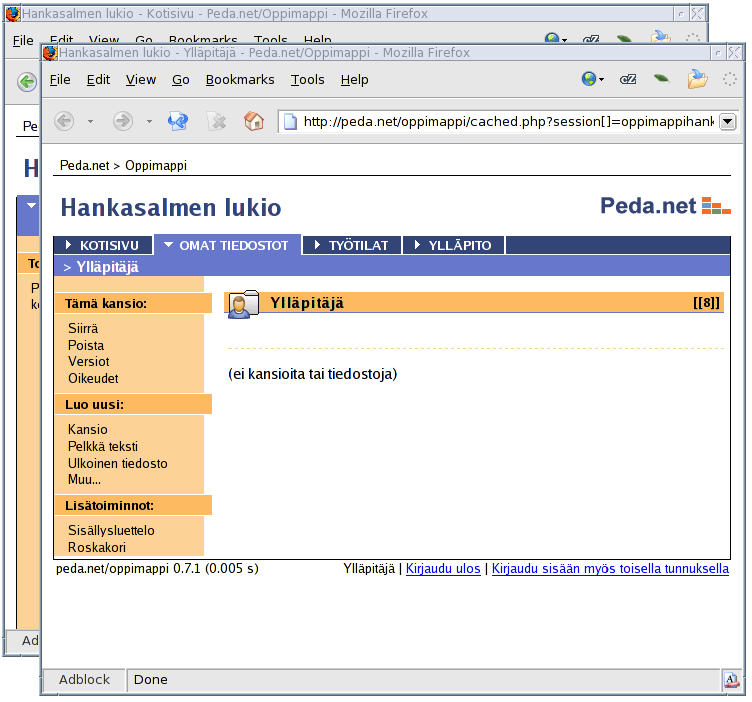
\includegraphics[width=10cm]{kuvat/oppimappi-new-window}
\caption{Oppimappi: linkin avaaminen uudessa ikkunassa}
\label{fig:oppimappi-new-window}
\end{kuva}

Oppimappia voidaan arvioida my�s luvussa
\ref{label:kaytettavyydessa_huomioitavaa} esitettyjen kohtien
perusteella:

\begin{description}

\item[ulkon��n taitto] Oppimapissa oletuksena k�ytetty tyylitiedosto
mukailee Peda.net-hankkeen staattisia www"-sivuja. Kirjasimeksi on
valittu groteski kirjasinleikkaus, sill� se on yleens� n�yt�ll�
paremmin luettava kuin antiikva. Tekstin kokoa ei ole m��ritelty
absoluuttisesti vaan leip�teksti on k�ytt�j�n selaimen oletuskoko.
Oikein konfiguroitu www-selain k�ytt�� siis aina optimaalista tekstin
kokoa. K�ytt�j� voi halutessaan k�ytt�� omaa CSS-tyylitiedostoa.

\item[yhdenmukaisuus] Koko sovelluksen ulkon�k� on m��ritelty yhdess�
CSS-tyylitiedostossa. Koska HTML"-koodissa ei ole m��ritelty ulkoasua
vaan ainoastaan sis�ll�n rakenne ovat kaikki sivut kesken��n
yhdenmukaisia. Kaikki sis�ll�n muokkaus tapahtuu toiminta"-palkin
kautta ja toiminnot tallennetaan aina lomakkeen lopussa olevasta
``Tallenna''-painikkeella. Mik��n, mik� ei n�yt� painikkeelta ei tee
j�rjestelm��n pysyvi�, kaikkia k�ytt�ji� koskevia muutoksia ja
toisaalta kaikkien painikkeiden painaminen tekee pysyvi� muutoksia.

\item[saavutettavuus] Oppimapin sis�lt� on esitetty semanttisella
merkinn�ll� ja esimerkiksi sivun ulkoasua ei ole tehty taulukolla.
T�m�n ansioista k�ytt� esimerkiksi puheselaimella onnistuu hyvin.
Samoin kirjasinkokoa voi vapaasti muuttaa ja sovellus k�ytt��
selaimessa asetettua tekstin kokoa. Suurta teksti� tarvitseva k�ytt�j�
on jo aikaisemmin s��t�nyt selaimensa haluamakseen.

\item[personalisointi] Oppimappi tarjoaa mahdollisuuden vaihtaa
k�ytt�liittym�n ulkoasua (k�ytt�j� voi valita ulkon��n vaihtoehtoisista
CSS-tyylisivuista) ja k�ytt�liittym�n kielt�. Lis�ksi j�rjestelm� ker��
tapahtumahistoriaa k�ytt�jien toimista.

\item[tehokkuus] Oppimapin vasteaika on keskim��rin 0,04 sekuntia sivua
kohden. Keskim��r�inen sivu on noin 20 kilotavua, mutta tiedonsiirrossa
k�ytet��n gzip"-pakkausta, jos selain sit� tukee, jonka ansiosta
siirrett�v�n datan m��r� on noin 3 kilotavua sivua kohden. Tavallisella
modeemillakin sivun pit�isi siis saapua aina alle 2 sekunnissa. Sivun
ulkon�k��n vaikuttava CSS-tiedosto ja ikonit tarvitsee siirt�� vain
ensimm�isell� sivulla, sen j�lkeen ne ovat selaimen v�limuistissa.

\item[sis�lt�] Peda.net ei ota kantaa Oppimapilla tuotettavaan
sis�lt��n. K�ytt�liittym�n tekstit yll�pidet��n keskitetysti Peda.netin
toimesta ja eri kieliversioita tehd��n k�ytt�jien tarpeiden mukaan.
Useinmmissa tapauksissa joku Peda.netin k�ytt�jist� tarjoutuu
k��nt�m��n tarvittavat merkkijonot uuden kielen tukemista varten.

\item[luotettavuus] Oppimappi ei ole ollut viel� k�yt�ss� riitt�v�n
kauan, ett� toimintavarmuudesta voitaisiin sanoa mit��n tarkkaa.
Kuormitustestiss� j�rjestelm� pystyy nykyisell� palvelimella tarjoamaan
l�hes 30 sivua sekunnissa jatkuvasti. J�rjestelm� on ollut t�t�
kirjoitettaessa tuotantok�yt�ss� kaksi viikkoa ilman huoltotaukoja.

\item[navigointi] Oppimappi tarjoaa koko ajan linkit koko hierarkian
p��tasoille (kotisivu, omat tiedostot, ty�tilat ja yll�pito) ja muuten
hierarkiassa edet��n yksi taso kerrallaan alasp�in tai palaamalla
suoraan mille tahansa edelliselle tasolle.

\end{description}

\subsection{Johtop��t�ksi� Oppimapin k�ytett�vyydest�}
\label{oppimapin-kaytettavyys-yhteenveto}

Yhteenvetona vaikuttaisi silt�, ett� k�ytett�vyyden kannalta ainakin
CSS-tyylisivuja pit�isi viel� kehitt��. Erityisesti ikkunan pinta-ala
on nyt tehottomassa k�yt�ss�, mutta sen korjaamiseksi t�ytyy poiketa
usein k�ytetyst� www"-sivustojen taitosta ja on vaikea sanoa ilman
tarkempaa tutkimusta onko k�ytett�vyyden kannalta parempi, ett� sivu
n�ytt�� samanlaiselta kuin muutkin, vai ett� sen k�yt�n tehokkuus on
teoriassa maksimaalinen. Samoin k�ytett�vyytt� puheselaimilla ja
braille"-n�yt�ill� pit�isi tutkia viel� tarkemmin.

Toiminnallisesti Oppimapissa on puutteena my�s t�ysi rinnakkaisten
muutosten hallinta. Tietokantaan tehd��n lukituksia vain tiedon eheyden
varmistamiseksi tallennuksen yhteydess�. Etuna on, ett� mit� tahansa
tiedostoa voi muokata milloin tahansa, mutta jos samaa dokumenttia
muokkaa samaan aikaan kaksi eri henkil��, eiv�t muutokset yhdisty
automaattisesti. Ainoastaan viimeisen� tallennettu versio j�� voimaan.
Versionhallinnan ansiosta vanhempikin versio j�� j�rjestelm��n, mutta
muutoksien yhdist�minen pit�� tehd� j�lkik�teen k�sity�n�. Koska
j�rjestelm� pit�� kirjaa my�s vanhoista versioista, tulevaisuudessa on
mahdollista tehd� koneellinen muutosten yhdist�minen, jos eri
henkil�iden tekem�t muutokset eiv�t ole ristiriidassa kesken��n.
\cite{ritcher:three-way-merge}

Toinen merkitt�v� puute on rinnakkaisissa muutoksissa tilanne, jossa
henkil� A aloittaa dokumentin X muokkaamisen ja t�m�n j�lkeen henkil� B
poistaa dokumentin X. Virhetilannetta, jossa dokumentin X muutokset
yritet��n tallentaa, mutta dokumenttia X ei ole en�� olemassa, ei
ainakaan toistaiseksi k�sitell�. Ongelmana on, pit�isik� j�rjestelm�n
palauttaa dokumentti X j�rjestelm��n (miten? Eik� dokumenttia X voikaan
oikeasti koskaan poistaa?) ja tallentaa muutos. Vai pit�isik� muutokset
tallentaa uutena dokumenttina? Jos, niin minne ja mill� nimell�?


\subsection{Vihko}
\label{pedanet-vihko}

Peda.net Vihko on kirjoittajan nykyinen kehitysprojekti, joka tarjoaa yksitt�isen koulun kaikille kursseille riitt�v�n oppimisymp�rist�n.T�m� sovellus ei tue kurssien j�rjest�mist� usean eri oppilaitoksen kesken, vaan on suunniteltu yksitt�isen koulun tarpeita varten. Rajaukseen p��dyttiin, koska ohjelman toteuttamisen ty�m��r�n arvioitiin kasvavan liian suureksi nykyisiin resursseihin verrattuna. Sovellusta on kehitetty kes�st� 2003 alkaen ja sen arvioitu julkaisuajankohta on syksyll� 2004. Kuten selaink�ytt�iset sovellukset yleens�, julkaisu ei tarkoita sovelluksen kehityksen lopettamista. Uusia ominaisuuksia tullaan lis��m��n julkaisun j�lkeen k�ytt�jien toiveiden mukaan.

Yll�pit�j�n kannalta merkitt�vi� ominaisuuksia ovat k�ytt�jien hallinta monitasoisten ryhmien kautta, kurssien ja kurssimateriaalien oikeuksien m��rittely luku- ja kirjoitusoikeuksien avulla ja versionhallinta sek� kaiken materiaalin vapaa linkitt�minen mihin tahansa j�rjestelm�n sis�ll�. Loogisella tasolla vihkossa yll�pidet��n kaksisuuntaista hierarkiaa, joka muodostuu erilaisista dokumenttityypeist� tai moduuleista: kansioista, tiedostoista, keskusteluista ja ty�tiloista. Jokainen moduuli voi sis�lt�� muita moduuleita ja jokainen moduuli voi n�ky� monen eri moduulin sis�ll�. Tietokanta mahdollistaa jopa moduulin n�kymisen itsens� sis�ll�. Osaa toiminnoista on rajoitettu k�ytt�j�n toimien helpottamiseksi.

Vihkon k�ytt�liittym�n p��osat muodostuvat navigointipalkista, toimintovalikosta ja sis�lt�alueesta. Kuvassa \ref{fig:vihko1} n�kyy Vihkon ty�p�yt�-n�kym�. T�m� on Vihkon aloitussivu sis��nkirjautumisen j�lkeen. Yl�reunassa n�kyy Vihkon otsikko (t�ss� esimerkiss� ''Testiymp�rist� 0.5.3+'') ja linkit eri alueille Vihkon sis�ll�: ty�p�yt�, omat tiedostot, ty�kalut ja yll�pito. Vasemman reunan palkissa on aina sen hetkist� sis�lt�� koskevat toiminnot, t�ss� tapauksessa  vain ''palauta poistetut kohteet'', joka palauttaisi sis�lt�listaukseen ne dokumentit, ty�tilat ja kansiot, jotka k�ytt�j� on aikaisemmin itse poistanut. Itse sis�lt�alue muodostuu t�ll� sivulla erilaisista objekteista, joilla jokaisella on ikoni, nimi, kuvaus ja toimintoja. Nimest� n�p�ytt�m�ll� p��see k�ytt�m��n objektia ja objektin per�ss� olevaa toimintoa k�ytt�m�ll� sen ominaisuuksiin voi vaikuttaa.

\begin{kuva}
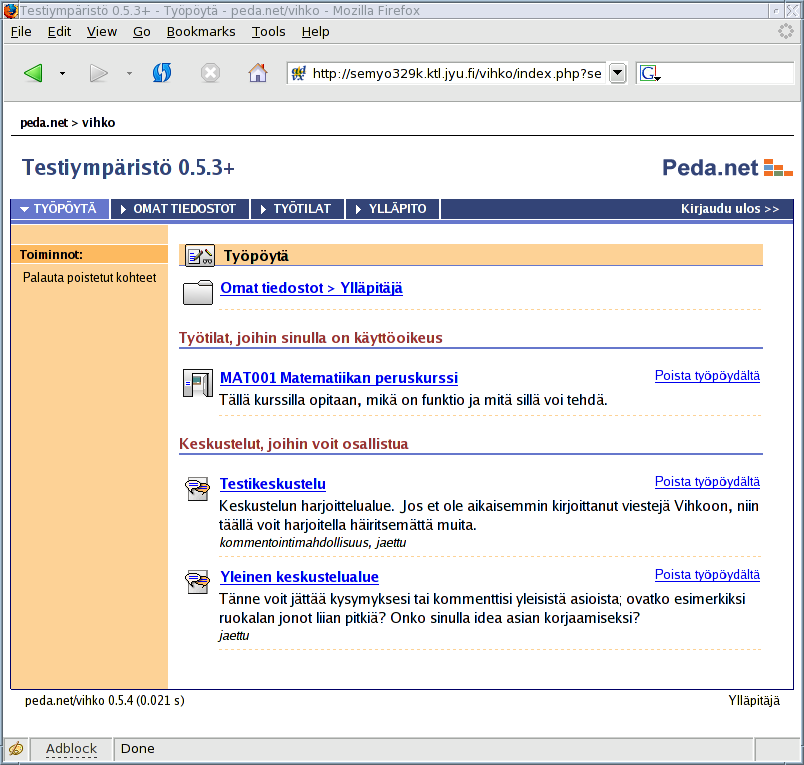
\includegraphics[width=10cm]{kuvat/vihko1}
\caption{Vihko: ty�p�yt�-n�kym�}
\label{fig:vihko1}
\end{kuva}

\begin{kuva}
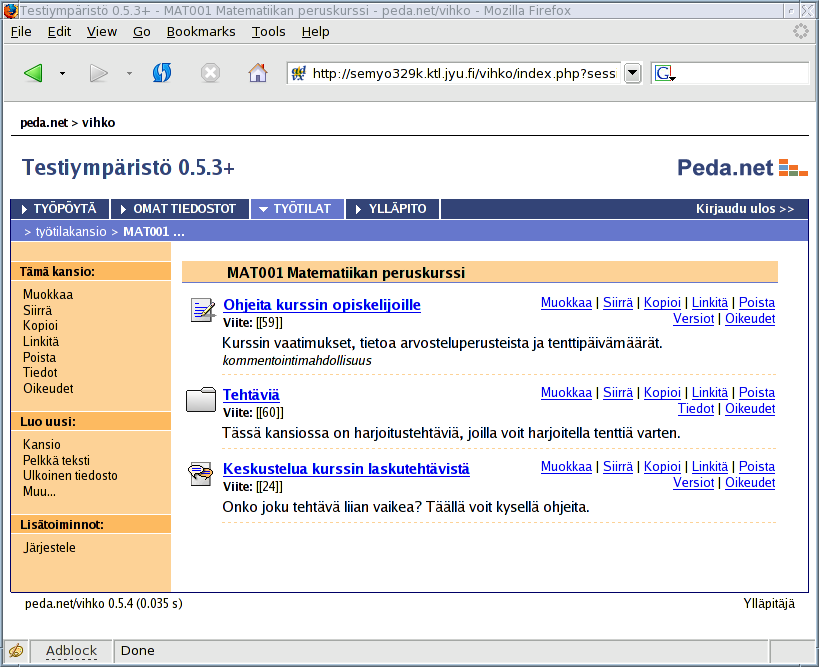
\includegraphics[width=10cm]{kuvat/vihko-kansio}
\caption{Vihko: esimerkki kurssin sis�ll�st�}
\label{fig:vihko-kansio}
\end{kuva}

\begin{kuva}
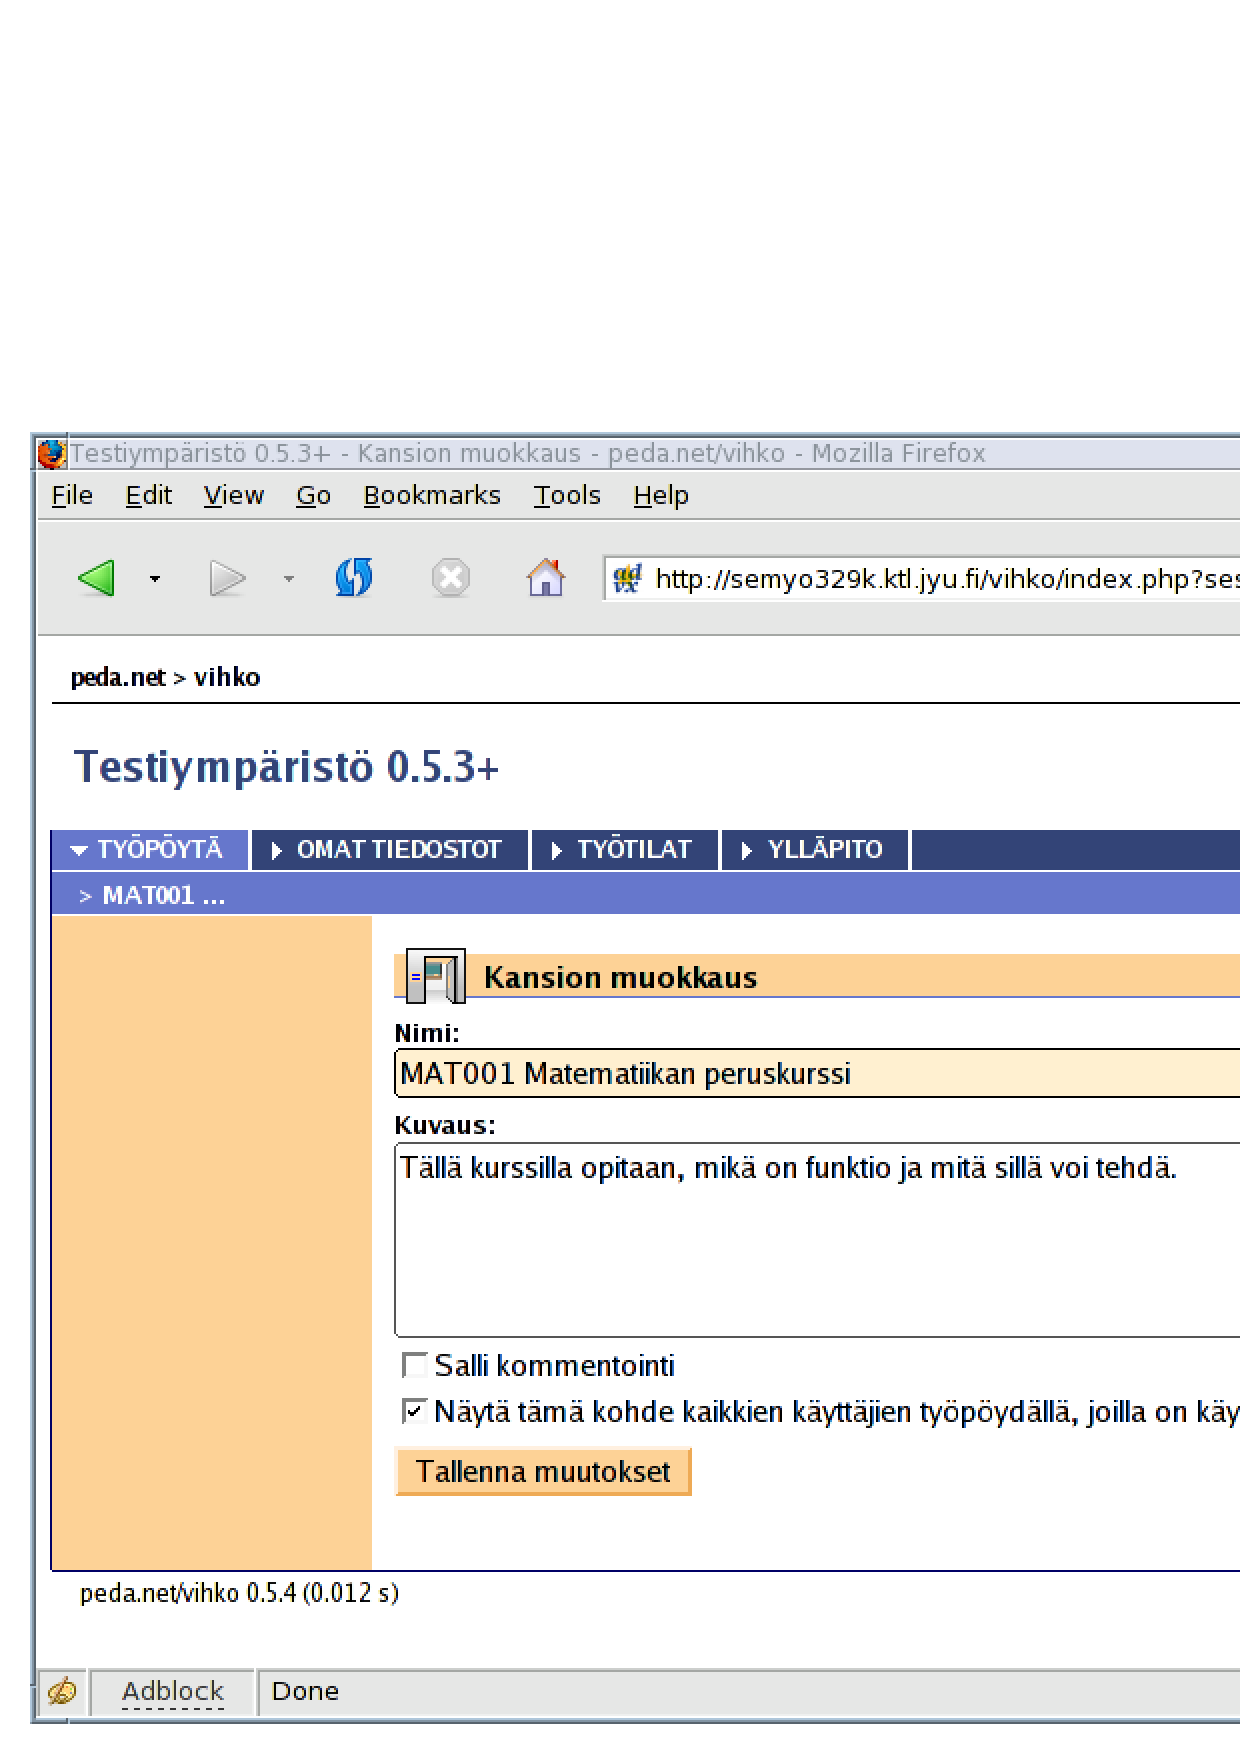
\includegraphics[width=10cm]{kuvat/vihko2}
\caption{Vihko: esimerkki kansion tietojen muokkaamisesta}
\label{fig:vihko2}
\end{kuva}

Jos opettaja siirtyy esimerkiksi matematiikan kurssille, annettaisiin h�nelle kuvan \ref{fig:vihko-kansio} mukainen n�kym�. T�ss� vasemmassa reunassa on edelleen yleisi� toimintoja, jotka koskevat t�t� kurssia (tai kansiota). Lis�ksi jokaisen kansion sis�ll� olevan objektin per�ss� on oikopolut vastaaviin useimmin k�ytettyihin toimintoihin; jos k�ytt�j� n�p�ytt�� jonkin kansion sis�ll� olevan objektin nime�, siirtyy h�n sen objektin omaan n�kym��n, jossa t�m�n n�kym�n oikopolut l�ytyisiv�t sen n�kym�n vasemman reunan toimintopalkista. Jos k�ytt�j� valitsee ''Teht�vi�''-kansion per�ss� olevan ''Muokkaa''-toiminnon, p��see h�n muokkaamaan kansion tietoja kuvassa \ref{fig:vihko2} esitetyn k�ytt�liittym�n kautta. Tai, jos k�ytt�j� valitsee esimerkiksi vasemman reunan palkista kohdan ''Luo uusi: tekstitiedosto'', p��see h�n kuvan \ref{fig:vihko3} kaltaiseen n�kym��n.

\begin{kuva}
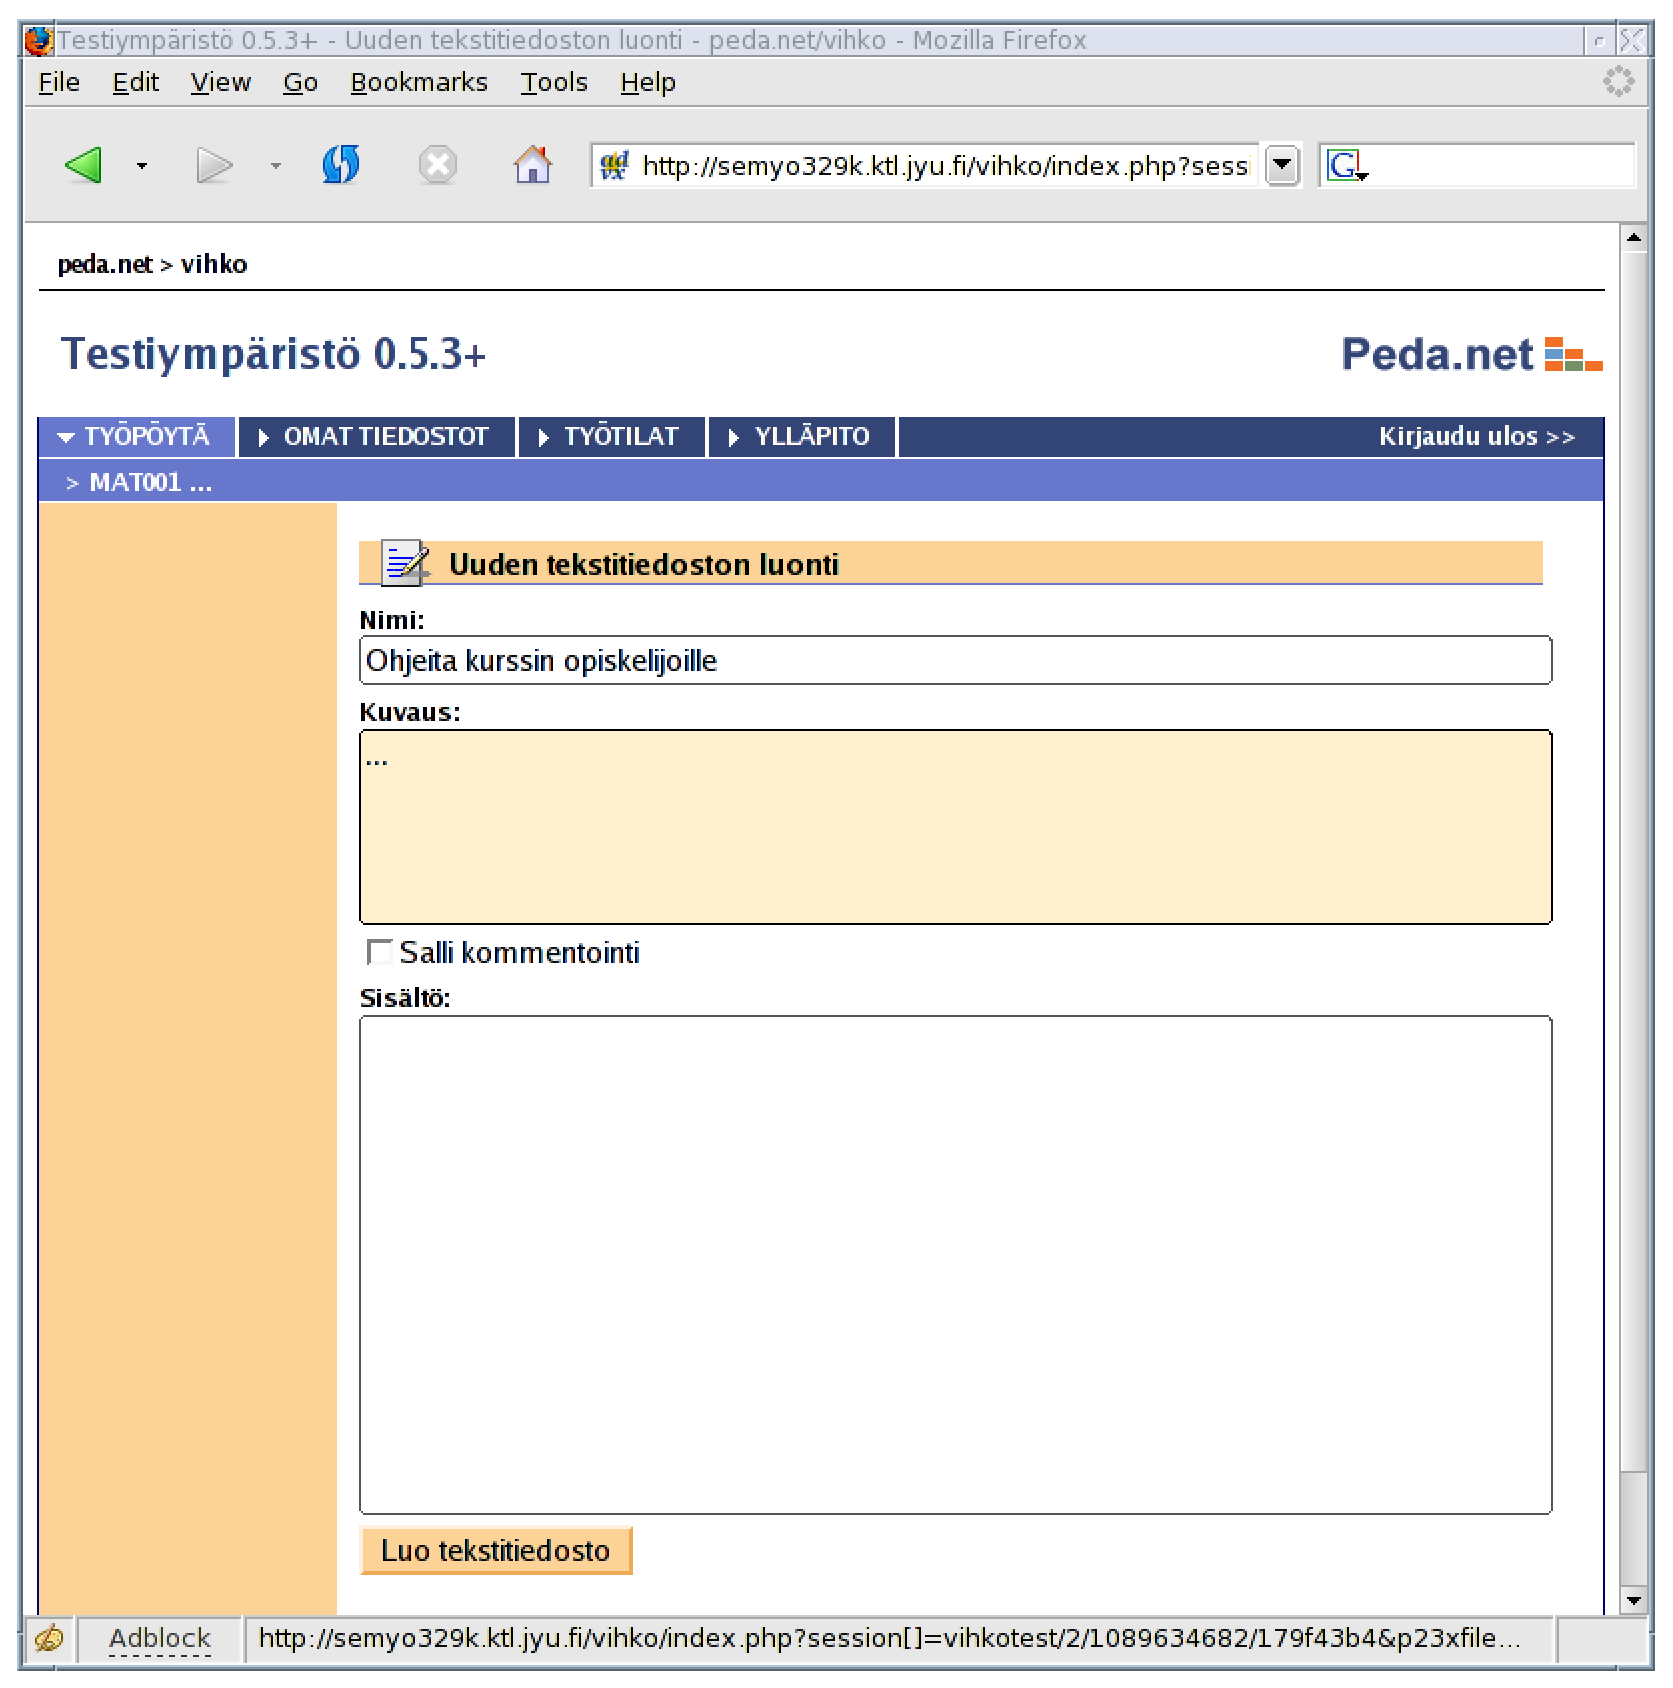
\includegraphics[width=10cm]{kuvat/vihko3}
\caption{Vihko: uuden kansion luontin�kym�}
\label{fig:vihko3}
\end{kuva}

Vaihtoehtoisesti k�ytt�j� voi n�p�ytt�� vain ''Ohjeita kurssin opiskelijoille''-tiedoston nime�, jolloin t�m� tiedosto asetetaan aktiiviseksi n�kym�ksi (katso kuva \ref{fig:vihko4}). T�ll�inkin t�t� objektia (tekstitiedostoa) koskevat toiminnot l�ytyv�t vasemman laidan toimintovalikosta ja sis�lt� n�kyy valkoisella pohjalla sis�lt�alueella. T�ss� esimerkiss� on sallittu my�s tiedoston kommentointi: lukija voi j�tt�� kommentin tiedoston sis�lt��n liittyen.

\begin{kuva}
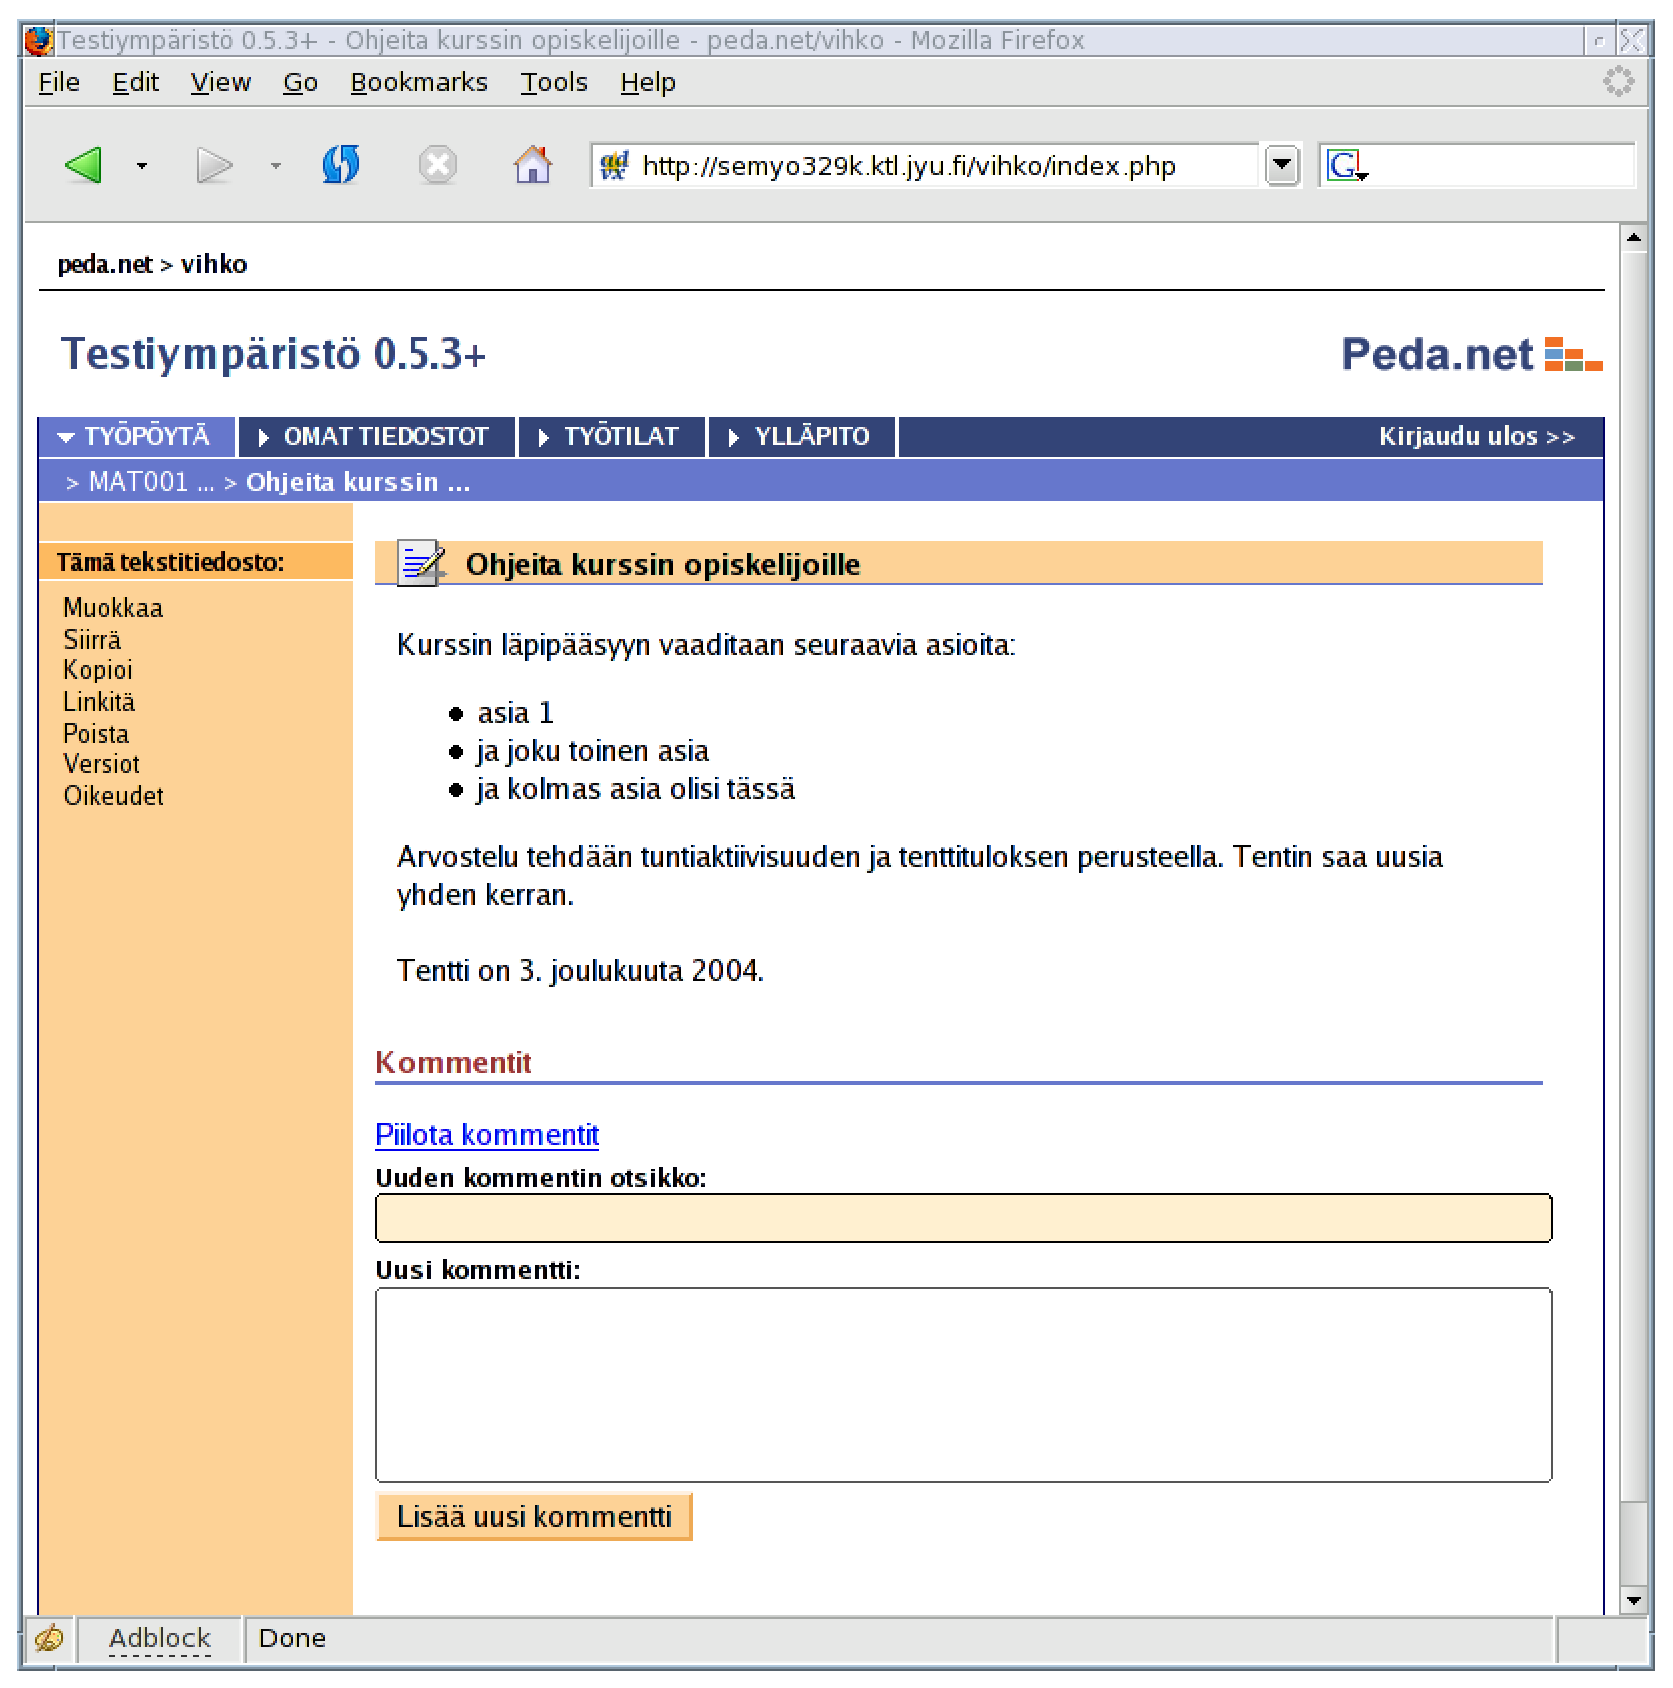
\includegraphics[width=9cm]{kuvat/vihko4}
\caption{Vihko: esimerkki tekstitiedostosta}
\label{fig:vihko4}
\end{kuva}

Valitsemalla vasemman reunan toiminnoista kohdan ''Versiot'', k�ytt�j� p��see katselemaan saman dokumentin vanhoja versioita. Vanhoista versioista vai esimerkiksi virheellisen muokkauksen tehty��n hakea haluamansa kohdan takaisin. Lis�ksi tiedoston voi haarauttaa: vanhan version voi kopioida uudeksi tiedostoksi. Tulevaisuudessa t�h�n on tarkoitus tehd� viel� k�ytt�liittym�, joka esitt�� paremmin dokumentin historian, jos se on haarautettu useaksi tiedostoksi, tai jos nykyinen tiedosto on jonkin muun dokumentin haara.

T�ss� n�kym�ss� listataan my�s dokumentin sijainnit: koska dokumentin tai kansion voi \emph{linkitt��} n�kym��n miss� tahansa, on mahdollista, ett� tiedosto n�kyisi esimerkiksi Matin omissa tiedostoissa samaan aikaan kun se n�kyy Matin pit�m�n kurssin kurssimateriaalina. Merkitt�v�n� erona moneen muuhun j�rjestelm�n, vihkossa my�s kansioita voi linkitt��. T�m�n seurauksena esimerkiksi tiedoston poistamisessa j�rjestelm�n t�ytyy tutkia, n�kyyk� tiedosto monessa eri paikassa. Olisi k�ytt�j�n kannalta ik�v��, jos h�n vahingossa poistaisi jonkin tiedoston, koska luuli sen olevan ainoastaan h�nen omissa tiedostoissaan, kun se todellisuudessa n�kyikin my�s h�nen pit�m�ns� kurssin er��ss� kansiossa. Toisaalta, jos tiedosto halutaan lopullisesti poistaa, on t�rke��, ett� k�ytt�j� voi poistaa tiedoston yhdell� toiminnolla riippumatta siit�, n�kyyk� se monessa eri paikassa.

\begin{kuva}
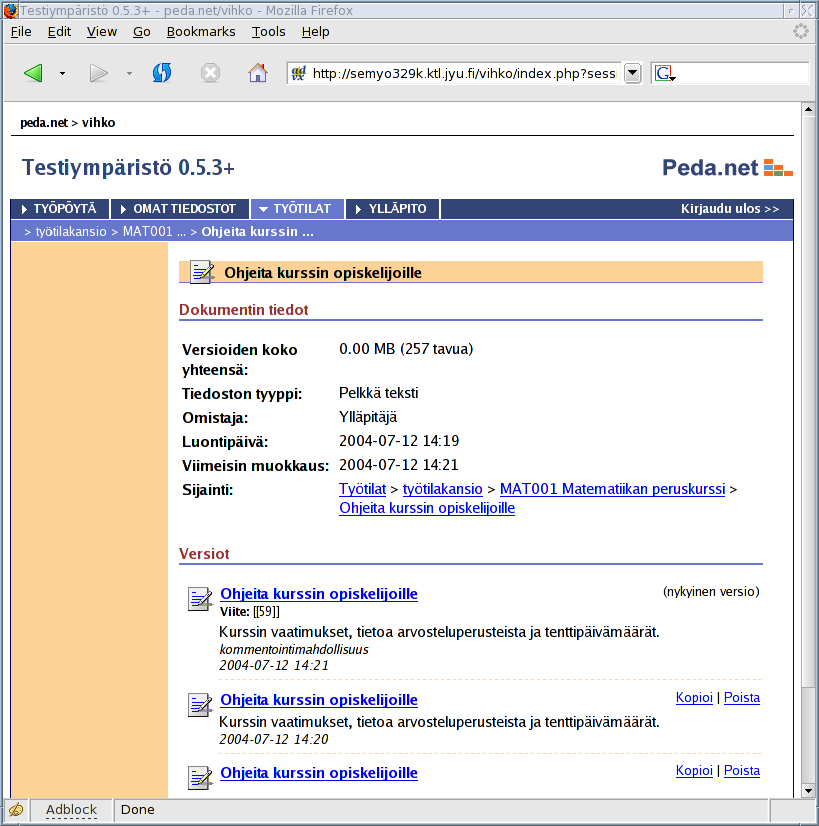
\includegraphics[width=9cm]{kuvat/vihko5}
\caption{Vihko: tekstitiedoston versioita}
\label{fig:vihko5}
\end{kuva}



\chapter*{Kiitokset}

Matthieu Weber ja Antti-Juhani Kaijanaho ovat tuottaneet
\LaTeX{}-luokan Pro Gradu -tutkielmia varten, jota my�s t�m� dokumentti
k�ytt��. XXX ja YYY oikolukivat tutkielman. Kiitokset heille!


%\cite{refresh} -- REFRESH BIBLIOGRAPHY (Makefile trigger)
%%% Bibliography:
\bibliographystyle{bibtexstyle}
\bibliography{bibliography}

\end{document}
